\documentclass[12pt,a4paper]{article}

\usepackage[dvips]{graphicx}
\usepackage[dvips]{color}
\usepackage{amsbsy, marvosym}
\usepackage{amsmath}
\usepackage{paralist}
%\usepackage{algorithm2e}
\usepackage{algorithmic}
\usepackage{algorithm}
\usepackage{subfigure}
\usepackage{lscape}
\usepackage{booktabs}
\usepackage{lscape}

\newcommand{\HRule}{\rule{\linewidth}{0.5mm}}

\pagestyle{plain}
\textwidth 16cm
\textheight 23cm
\oddsidemargin -0.5cm
\evensidemargin -0.5cm
\topmargin 0cm

\numberwithin{figure}{section}
\numberwithin{table}{section}
\numberwithin{algorithm}{section}

\usepackage{float}
\floatstyle{ruled}
\newfloat{program}{thp}{lop}[section]
\floatname{program}{Program}

\newfloat{note}{thp}{lon}[section]
\floatname{note}{Note}

\begin{document}
\pagenumbering{arabic}
\setlength{\parindent}{5mm}
\setlength{\parskip}{10pt plus2mm minus2mm}
\thispagestyle{empty}
% TITLE

\begin{titlepage}
 
\begin{center}
 
% Upper part of the page
%\includegraphics[width=0.15\textwidth]{./logo}\\[1cm]
 
\textsc{\LARGE Liverpool John Moores University}\\[1.5cm]
 
\textsc{\Large Ph.D Thesis}\\[0.5cm]
 
 
% Title
\HRule \\[0.4cm]
{ \Large \bfseries Adaptive Optimal Telescope Scheduling}\\[0.4cm]
 
\HRule \\[1.5cm]
 
% Author and supervisor
\begin{minipage}{0.4\textwidth}
\begin{flushleft} \large
\emph{Author:}\\
Stephen \textsc{Fraser}
\end{flushleft}
\end{minipage}
\begin{minipage}{0.4\textwidth}
\begin{flushright} \large
\emph{Supervisor:} \\
Prof. Iain \textsc{Steele}
\end{flushright}
\end{minipage}
 
\vfill
 
% Bottom of the page
{\large \today}
 
\end{center}
 
\end{titlepage}

%\title{Adaptive Optimal Telescope Scheduling
%Ph.D Thesis}
%\author{S.N. Fraser}
%\date{\today}
%\maketitle

\begin{abstract}
Astronomical telescopes operate in a dynamic and uncertain operational environment. Time is often oversubscribed with programs competing for available slots and the best observing conditions. In order to achieve a high scientific return a scheduler must be able to create a globally optimal observing schedule. 

Using data collected from external sources and embedded instrumentation I investigate and characterize the scheduler's operating environment. I investigate metrics for characterizing the value of schedules both locally (at the decision point) and over longer horizons. Using this information an extensible software architecture is designed incorporating a simulation framework to allow a variety of schedulers and environmental scenarios to be constructed.

 Experiments are performed using the scheduler component architecture and simulation framework to determine the effects on schedule quality of environmental stability, disruptive events and reliability of prediction under a range of load conditions. 

%metrics 
Investigations into the effects of choice of selection scoring metric on the final quality of schedules showed that contrary to an initial opinion that it should be feasible to find a single candidate quality metric with which to evaluate schedule quality, there is in fact no clear candidate as an absolute quality metric. The choice of weighting of the selection metrics determines the character of the schedule but only the dominant scoring metric has any real effect while the other metrics simply manifest themselves as noise.

%stab reliable 0.7/0.8
It was found that where conditions are relatively stable there is an advantage to using longer look-ahead horizons but that where conditions are unstable or disruptive a basic despatch scheduler achieves results as good or better. A look-ahead scheduler with a horizon of 4 hours can give an improvement of upto 23\% over a simple despatch scheduler when seeing remains stable over a period of upto 6 hours.

Experiments performed to determine the effect of chosing a suitable look-ahead horizon based on the perceived stability of environmental conditions have shown that when determining the length of this horizon, if we either over or under-estimate the duration of stable conditions we obtain poorer results. When the stability length is severely under-estimated a loss of between 5\% and 17\% in quality was found to occur.  The optimum situation appears to be when the horizon is of order of or slightly less than the actual stability length. Where the stability length is over-estimated by a factor 2, a loss of 5\% to 10\% can occur.




\end{abstract}


\newpage
\tableofcontents
\newpage
\listoffigures
\newpage
\listoftables
\newpage
%\listof{program}{List of programs} 
\listofalgorithms

%\listof{note}{List of side-notes for me}

%\include{progex}

\section{Introduction}

\subsection{Background}
The Liverpool Telescope (LT) is a fully robotic 2 meter astronomical telescope situated at the Observatorio de los Roches de los Muchacos on La Palma in the Canary Islands. It operates without supervision, controlled by an integrated suite of software systems. The Robotic Control System (RCS) is responsible for deciding on the mode of operation and for protecting the telescope, it controls the telescope and its instruments and receives environmental information via a number of lower level subsystems. The Telescope Control System (TCS) is responsible for slewing the telescope axes onto targets and for tracking them through the night. The Instrument Control Systems (ICS) are responsible for configuration of the suite of scientific instruments, taking exposures, reading out, saving to disk and control of a realtime data reduction pipeline (DPRT). The Scheduler is a component of the Observer Support System (OSS) - DEFINE. 

The RCS makes requests to the scheduler at various times for groups of observations to perform. These are then executed and results reported back to the OSS. Observations specified by astronomers who have been allocated time, are stored in the Phase2 Observing Database (ODB) maintained by the OSS. The observation requests include all the information required to perform the observations - target location, instrument selection and configuration, exposure times etc. In addition a number of constraints are specified - time constraints determine when and how often the observations should be performed, observing constraints specify under what environmental conditions the observations may be performed - e.g. only if the target is above a certain elevation or when the \emph{seeing} is better than a specified level. User-specified QOS metrics define the acceptable levels of observation quality and regularity. 

The telescope operates in an uncertain environment \begin{inparaenum} \item availability is influenced by weather conditions (it does not open when there is rain, high humidity or extreme or gusting wind), \item at times the telescope may be \emph{taken over} by an external agenty \cite{xxx} (TOSA) to investigate \emph{targets-of-opportunity}, \item engineering work must be scheduled in at various times, \item there are the inevitable and unexpected downtime due to software and hardware faults, \item atmospheric conditions which constrain the choice of available observation can change over short timescales, \item observation requests can arrive in the database or be removed or modified at any time \end{inparaenum}. These factors make it difficult to make long term scheduling commitments with any chance of success.

\cite{steele97control} have defined a series of ?characteristics? that can contribute to a \emph{good} schedule. They mention fairness (of time allocations between various committees), efficiency (quality of observations, minimization of idle time) and feasibility (is the target visible).

First version of scheduler \cite{fraser04scheduling} is a simple despatch scheduler which uses an objective function formed using a weighted sum of metrics.
Describe the scheduler as candidate selection then application of metrics (leave gory details till later). A full search of the ODB is performed, enabled candidate groups are extracted and scored using a weighted sum of various metrics.

Does it work and how well, what problems - obviously needs imporvment or wouldnt be writing this..

\begin{itemize}
\item inefficient - need to call scheduler each time a group completes/fails.
\item obscure - dont know why decisions are being made - why g-1 and not g-2 selected.
\item suboptimal - just select best group now - no consideration of what next = local optimization.
\item difficult - how do we select the best relative weighting for metrics?.
\end{itemize}

How can we improve..
look at multiobject optimization \cite{silva04multiobjective} - very interesting. \cite{bresina95expected} deals with look-ahead and how improves qualities or metrics.

Say what these mean i.e for what will be doing - adaptive/learning, accountable (user-prefs), dispatch, predictive, lookahead, max utility,

i.e. blah blah - an adaptive scheduler will ... use of prediction to estimate likelihood of conditions for boosting future reward.. using dispatch because...the MEU theorem and decision thry....


\subsection{Scheduling in context}
Scheduling problem in general defined S+P+E+C - hierarchy, horizons, feedback/cyclic nature of process.

The aim of scheduling is to generate a schedule - this indicates what is to be done, when, and with which resource(s).Scheduling cannot however be considered in isolation, it is part of a hierarchy involving concepts such as planning and execution. In a machine environment there will also be a need to consider aspects of low level control and feedback.  
At some point the distinction between planning, scheduling and execution may become blurred depending on just how we characterize these. In highly dynamic environments planning, scheduling, execution and control may be continuous, interleaved or merged into a single operational \emph{entity} - better word?.

\begin{description}
\item[Scheduling] involves taking decisions regarding the allocation of available capacity or resources (equipment, personnel, space) to jobs, activities, tasks or customers over time. Scheduling thus results in a time-phased plan, or schedule of activities.

\item[Planning] involves the determination of the goals and objectives of an enterprise and the selection, through a systematic consideration of alternatives, of the policies, programs and procedures for achieving them. An activity devoted to clearly identifying, defining, and determining courses of action, before their initiation, necessary to achieve predetermined goals and objectives.

Planning is typically a long term activity - we define the term planning horizon as the period over which a plan is made or is expected to be of some utility in achieving its set out goals/objectives. Planning takes a global view of the enterprise, it may set targets to be achieved by the enterprise e.g. in the form of objective functions or the specification of constraints and preferences to be considered by lower layers. These goals may be somewhat imprecise or abstract - we are not deciding what to do when so much as what sort of things we want to do and how well we want to achieve them. 

We can usefully subdivide planning into several different horizons \cite{xxx} - these are by no means set in stone and more/fewer horizons may be more suited to specific enterprises. The precision of the objectives becomes more focused and the time span decreases as we move down the hierarchy \cite{chien00aspen}??

\begin{description}
\item[Strategic] horizon involves the creation of plans to cover very long periods of time. Typically this could be over a year or more and could at its most extreme represent the entire lifetime of an enterprise. 
\item[Tactical] horizon plans are designed to cover medium periods e.g. a semester on a telescope,  weekly or monthly production targets in factory.
\item[Operational] horizon plans are short term plans designed to allow an enterprise to function function, typically they cover the standard work-period of the enterprise e.g. a night's observing at a telescope, a shift at a factory.
\end{description}

\item[Execution] is the carrying out of the tasks assigned by the scheduler or planner by the enterprise - i.e. its normal operating procesdures. Execution may itself involve decomposition of assigned tasks, recovery from error or reaction to unexpected events.


\end{description}

Formally we shall define the scheduling problem with respect to the following structures:-

\begin{itemize}
\item A database, repository, queue or pool of tasks/jobs/activities $\mathbf{T}$ which are to be performed. This could be a set of observations by a telescope, processes on a computer, components to be manufactured in a factory, surgical operations to be performed in a hospital, blocks of trees to be felled in a forest. The pool of tasks may be static or dynamic, with new tasks inserted and uncompleted tasks removed while the execution is underway.

 \item A set of constraints $\mathbf{C}$ associated with the jobs - these may be \emph{unary} (limits on a single variable or resource e.g. $task_i$ must start between $t_1$ and $t_2$), \emph{binary} (linking the values of 2 variables - e.g. predecence $task_i$ must start before $task_j$ ) or may involve relationships between several problem variables. They may be further divided into:-
y\begin{description} 
\item[hard constraints] which must be guaranteed to be satisfied by a valid schedule, e.g. 
\begin{enumerate}
\item $task_i$ must be completed by latest finish time $lft_i$.
\item only 2 tasks can execute on $machine_y$ simultaneously.
\item there must be a gap of at least $t_{ij}$ between execution of $task_i$ and $task_j$.
\item $team_k$ cannot work more than $max_k$ hours in any day.
\end{enumerate}

\cite{sadeh91lookahead} and \cite{fox83thesis} define the following classes of constraints:-
\begin{itemize}
 \item  precedence constraints - describe
 \item  resource usage constraints - describe
 \item  many others - (see Fox paper).
\end{itemize}

 \item[soft constraints] or preferences which should be satisfied as far as possible but which are capable of relaxation to permit a feasible schedule to be derived. When relaxing constraints it is usual to associate a cost to the degree of relaxation, this  may be folded into the global objective function. The manner in which such relaxation occurs is likely to influence the search heuristics.
 (a list of examples here)
\begin{itemize}
 \item A telescope suffers from changes to \emph{seeing} due to turbulent motion of the atmosphere- some observations may have constraints which state they cannot be executed if the seeing is worse than $x$. 
 \item A machine in a factory may have a capacity which is determined by the current power levels or time of day.
 \item and another.
\end{itemize}

\end{description}

\item A set of resources $\mathbf{R}$ to assign to the tasks. e.g. a telescope or one of several observatories for performing the observations, a production line or machine to make the components, a team of lumberjacks to fell the blocks of tree, a surgical team to perform the operations.

\item A set of goals $\mathbf{G}$ which we are trying to achieve by performing these tasks. Goals may be specified in terms such as the standard measures from the CSP literature:- \emph{min-slack}, \emph{max-throughput}, \emph{min-tardiness}, or may be set out as objective functions to be maximized. Either way we need to be able to extract appropriate quality parameters from the schedule. 

\item The environment $\mathbf{E}$ in which the scheduler lives and which can influence the execution of the tasks and can change the goals. (list of examples plus refs- ) 

Environmental variables may be:- 

\begin{itemize}
  \item static - constant in time (telescope's elevation limit, number of processors).
  \item dynamic - changing in time (telescope's current azimuth, current instrument selection, etc).

These may further be classified as:-
\begin{itemize}
  \item deterministic - always known or predictable (e.g. position of the moon which affects sky-brightness and integration times, is always calculable).
  \item stochastic - randomly variable - (examples).
  \item chaotic - e.g. weather \cite{lorenz63npflow}, atmospheric seeing \cite{jorgenson91attractor}.
\end{itemize}
\end{itemize}

\end{itemize}

Scheduling may be divided into 2 sub-problems - the satisfycing problem consists of finding a schedule which satisfies the hard constraints i.e. all the tasks are assigned to a valid time slot without regard to preferences - we refer to this as a feasible schedule. Such a schedule may contain significant amounts of slack time (when no tasks are being performed) or under-utilization of resources - such schedules are generally inefficient but that may be all that is required - these problems may be represented as constraint satisfaction problems (CSP). The optimization problem consists of finding a schedule which is both feasible and achieves its goals as layed down by the soft-constraints whilst maximizing an objective function (or minimizing a cost function which is equivelent). We will refer to this as an optimal schedule and may be represented as a constraint optimization problem (COP). 

\subsection{Classification of scheduling problems}
Some ideas on classification of scheduling problems:-

\begin{description}
\item[Integration Depth] How much of the hierarchy of planning, scheduling, execution (and control) is involved and is there feedback and from/to which level(s).
\item[Flexibility] Are the results of the scheduling (i.e. the generated schedule to be followed) fixed or does it contain some flexibility. This may be in the form of temporal or resource assignment flexibility (windows in a fixed execution path) or a graph of multiple execution futures - i.e. contingency/redundancy .
\item[Proactive/reactive] Is the scheduling performed online or offline. ()Better name? - proactive at one end, reactive at other end of a scale)
\item[Method] Constructive or repair based, DDS is \emph{sort of} in between. Distributed techniques may confound this?. 
\item[Horizon] The time period or number of tasks over which the schedule is expected to be followed.
\item[Completeness] The number of tasks from the set of available/assignable tasks to insert into the schedule.
We can extract the following progression:-
\begin{enumerate}
\item Despatcher - Scheduler seeks the \emph{best} single task to perform from the set of assignable tasks at an instant.
\item Short Horizon - Scheduler selects a sequence of tasks from a subset of the assignable set to perform.
\item Complete - Scheduler must assign all assignable tasks.
\end{enumerate}
\end{description}

Note: In this scheme DDS is \emph{variable depth (typically S with feedback from E), neccessarily fixed, online with horizon $=$ 1 task, using a repair? based method}. 

Q:- What advantages/disadvantages do these measures convey - integrate into paras above?

Notes:- Completness/horizon - how do we determine the length of the horizon or do we select a subset of tasks from pool to execute over a horizon? Several ways:-
\begin{itemize}
\item Use knowledge of the environment dynamics and uncertainty in execution times to choose a \emph{hard-coded} horizon length.
\item Adaptively select horizon length from measured environment dynamics.
\item Use higher level goal-based planner to select a subset of pool for execution over the next horizon.
\item Combine the last 2.
\end{itemize}


\subsection{Constraint Satisfaction Techniques}

A constraint satisfaction problem (CSP) comprises:- A set $\mathbf{X} = \{x_i\}$ of variables over a set of domains $\mathbf{D} = \{d_i\}$ these may be continuous or discrete and bounded or unbounded and a set $\mathbf{C} = \{c_i\}$ of constraints on and between the variables that restrict the possible value assignments. A solution comprises an assignment of values from $\mathbf{D}$ to all the variables in $\mathbf{X}$ subject to $\mathbf{C}$. Further in an optimization problem the solution should maximize an objective function $F(\mathbf{X})$. A CSP may be represented as a directed graph in which the arcs represent constraint relationships between the variables represented as nodes. To represent a scheduling problem as a CSP the variables are identified as the tasks to be assigned time-slots from domains of available times. The objective function is a measure of the quality of the schedule.

   \begin{figure}[h]
   \begin{center}
   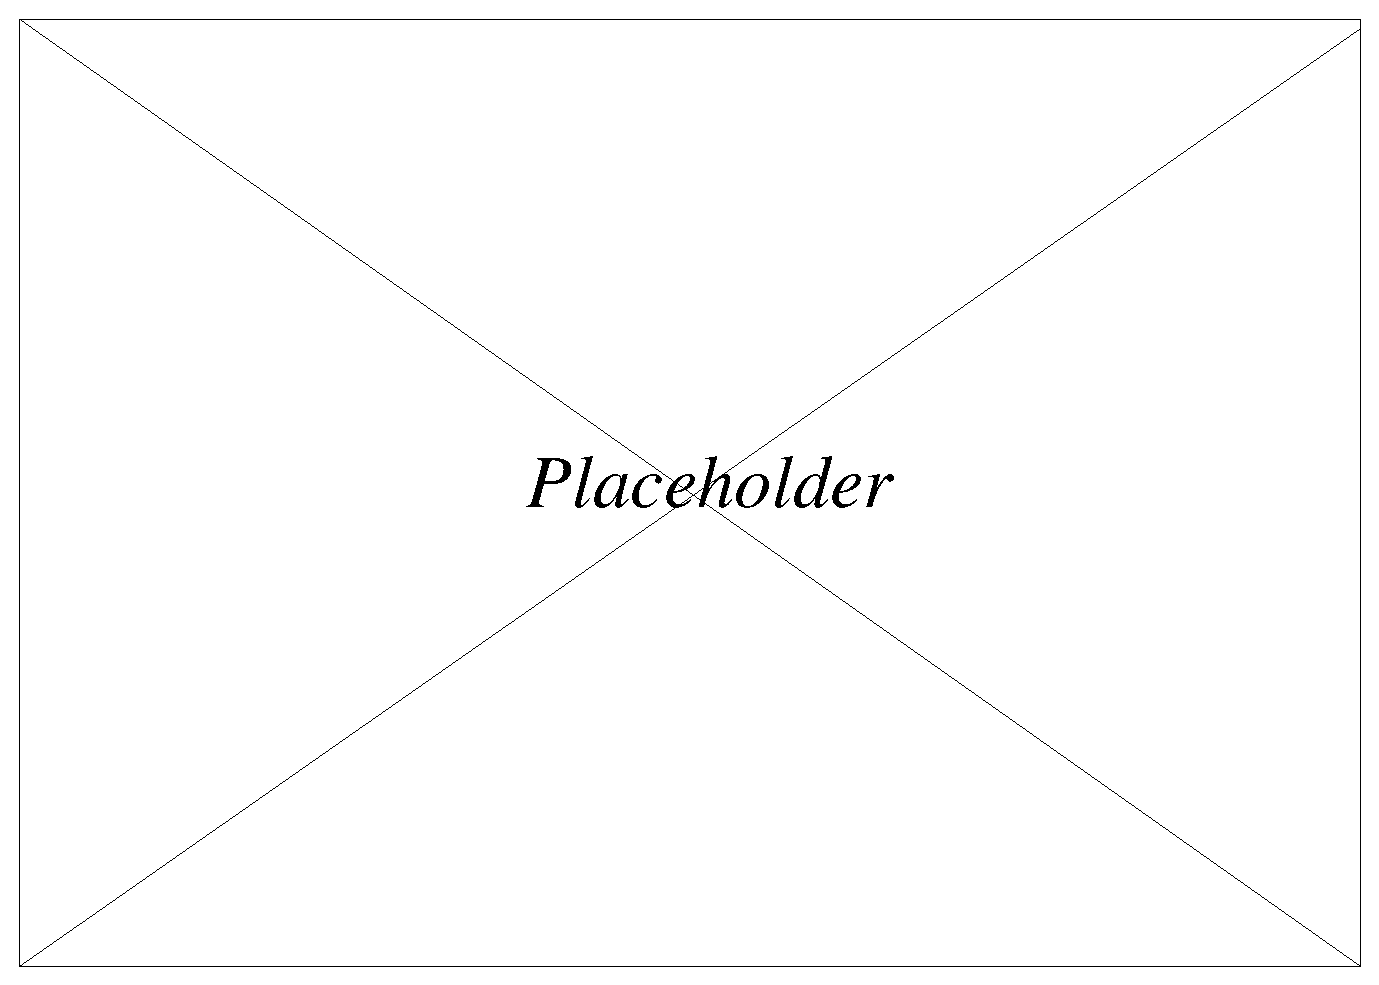
\includegraphics[height=6cm]{figures/placeholder.eps}
   \end{center}
   \label{fig:object} 
   \caption[Scheduling as a CSP.] 
   {Scheduling problem represented as a CSP graph with time-slot assignments (domains) for tasks (vars).}
   \end{figure} 


Solving scheduling as a CSP - 2 techniques have evolved - constructive techniques based on backtracking search from starting from an empty schedule, build up partial schedule by selecting a task and assigning a value from its available domain, check for consistency then onto next task. Keep going till hit deadend - no assignment of variable will allow progress. Then backtrack to last decision (assignment) and change. Uninformed backtracking typically requires $O(n!)$. In contrast, the repair technique starts with a fully built but typically inconsistent and suboptimal schedule. The technique then involves an iterative cycle of task retraction and re-assignment until all tasks are assigned and all constraints are satisfied. If optimization is required the objective function is measured at each cycle to check for improvment. The objective may also guide the search heuristics.



\subsection{Problem definition}
Detailed specification of observing requirements and what trying to do and what sent to RCS and what comes back- - RCS does task decomposition, it is the executor. include linked groups, sequencing 

Specific nomenclature/terminology and symbols that will be used hereafter.



The Phase 2 Observing Database (ODB) (see Fig.~\ref{fig:phase2-architecture}) contains details of all the programs of observations. These details are supplied by astronomers using external tools \cite{clayandfraser06tbd} or are generated by external intelligent agents \cite{xxx} (TEA).

   \begin{figure}[h]
   \begin{center}
   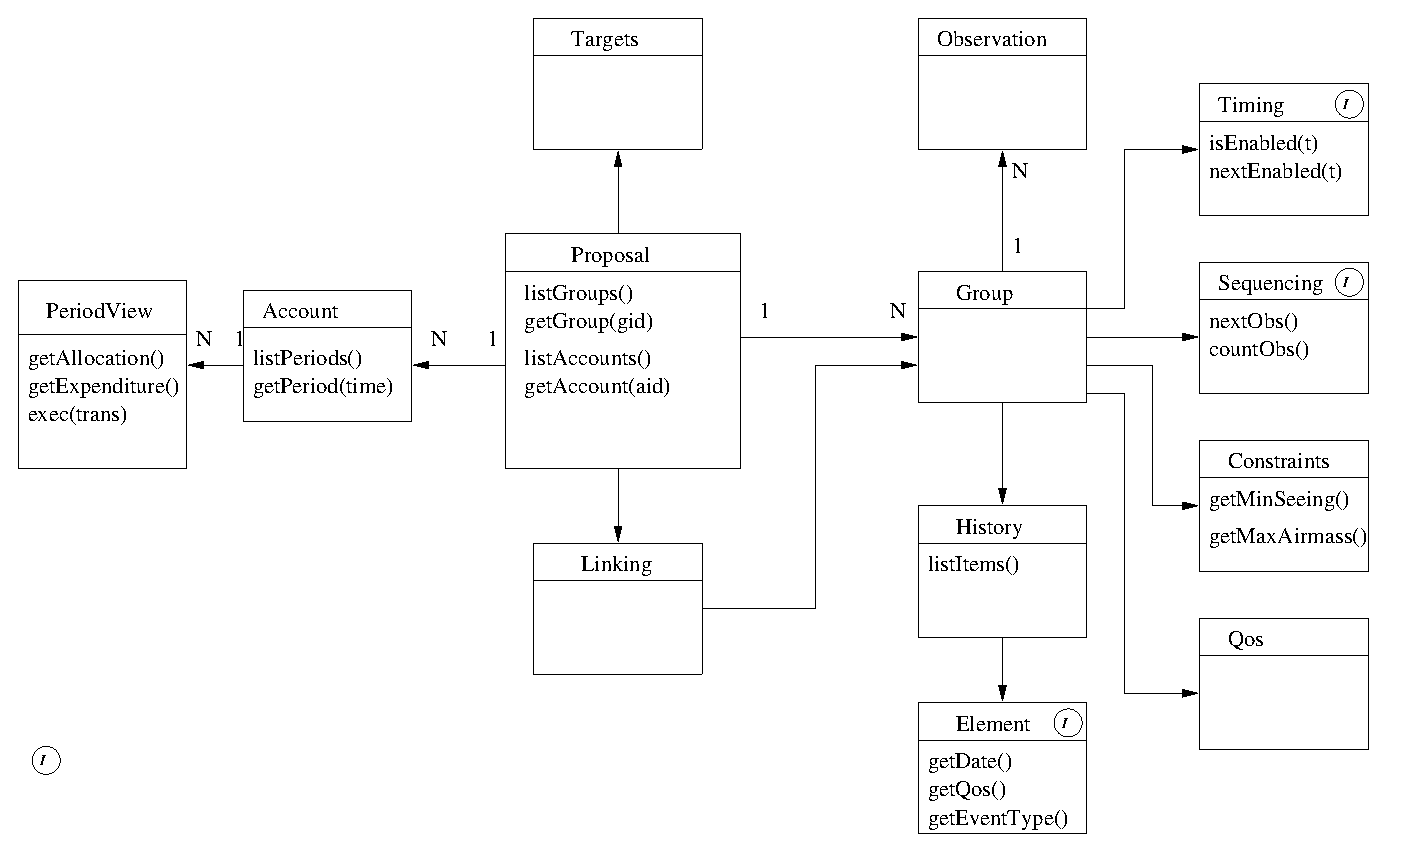
\includegraphics[height=6cm]{figures/phase2_architecture.eps}
   \end{center}
  
   \caption[Phase2 Architecture.] 
   {The Phase2 Observing Database (ODB) contains details of {\tt Proposals}, {\tt Groups} of {\tt Observations}, {\tt Accounting}, {\tt Linking}, {\tt Targets} and {\tt ExecutionHistory}..blah..blah.}
   \label{fig:phase2-architecture} 
   \end{figure} 

Proposals represent an astronomers observing program and correspond directly with the ?general definition? of a TAG allocated proposal. A proposal collects information required to perform the client's observations and time and resource accounting.  Programs collect together a number of different proposals for sharing of resource allocation. A proposal may participate in several programs. The unit of scheduling is termed a group and consists of the specifications of the observations, timing requirements, sequencing, observing condition constraints and quality of service metrics. Groups within a proposal may be linked in various ways (Fig.~\ref{fig:group-linking} contains details of some of these relationships.


   \begin{figure}[h]
   \begin{center}
   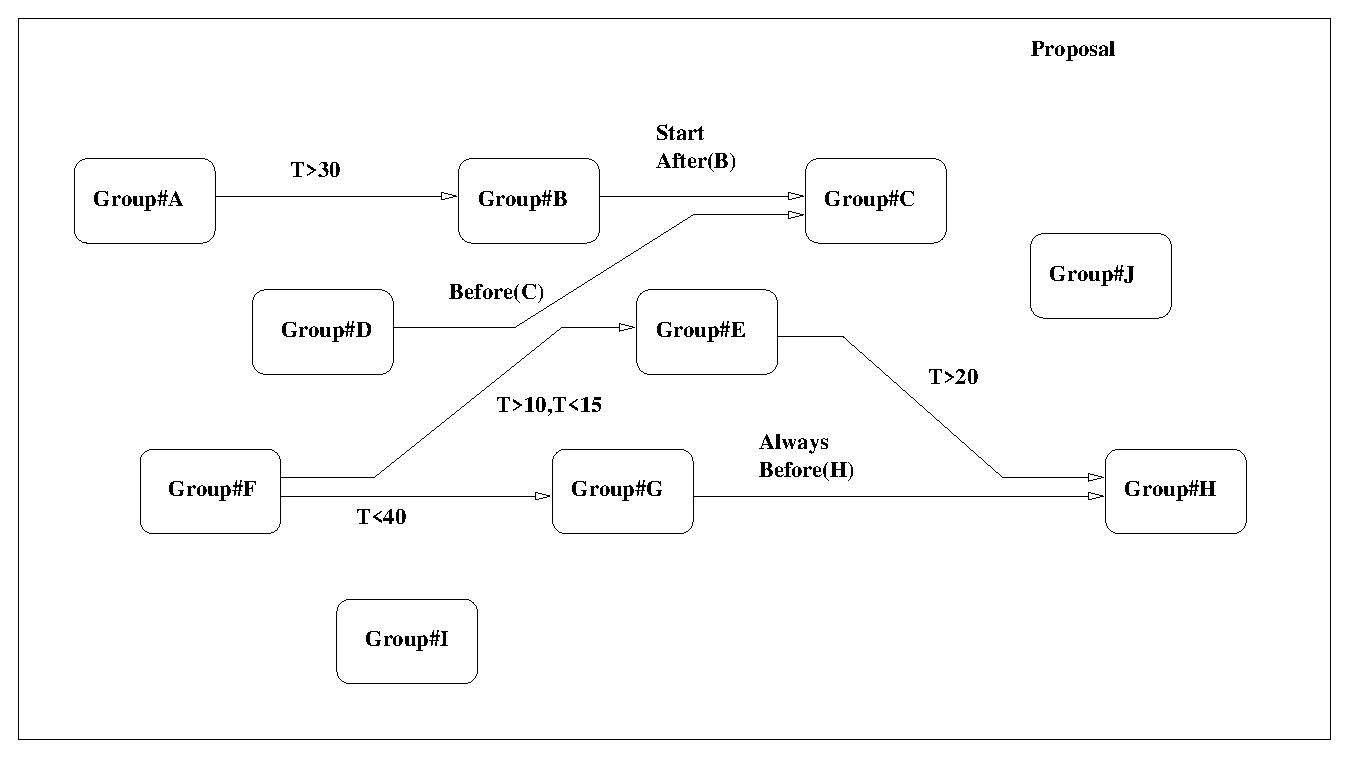
\includegraphics[height=6cm]{figures/group_linking.eps}
   \end{center}
  
   \caption[Group Linking.] 
   {Groups within a proposal may be linked in various ways. The constraint between {\bf Group\#A} and {\bf Group\#B} states that a {\bf Group\#B} cannot be executed unless a {\bf Group\#A} was executed at least 30 units earlier. The constraint between Groups {\bf \#C} and {\bf \#D} states that C should only be executed if D is able to be executed between 20 and 40 units later and requires the ability of the scheduler to predict future group enablement.}
   \label{fig:group-linking} 
   \end{figure} 


Each group has a set of enablement windows $E={e_i}$ which represent the intervals during which it should be observed if possible - these are obtained from the group's \texttt{TimeConstraints}, e.g. make this observation sometime between t1 and t2. As an added complication these may be cyclic - e.g. perform this observation once every 3 hours between t1 and t2. Some observations have fixed time constraints (do this at t3) or sliding fixed time constraints (do this at t1 or t2 or t3). 

The times when the group can actually be observed are further constrained by a number of factors:-
\begin{itemize}
\item Observations are only performed at night - in some cases we further restrict this to the period between evening and morning astronomical twilight.

\item Environmental constraints, some are deterministic e.g. only observe this target if the moon is greater than distance \emph{x} away from the target or only observe if the target is above elevation \emph{y}. Others are less predictable, e.g. only observe this target if the atmospheric seeing is less than \emph{z} arc seconds. 

\item Observations cannot be made during bad weather (the dome is closed to protect the instruments) and there is no point observing in cloudy conditions

\item There are unpredictable target-of-opportunity interrupts where external intelligent agents may take over the telescope for a period with no advance warning

\item There are certain periods, usually known in advance when the telescope is unavailable due to engineering or local or remote manual observing.

\end{itemize}

Taken together these result in considerable uncertainty in the time spans available for observing (active windows). In such a dynamic environment any advanced planning can become rapidly out of date. 


The figures below illustrate 2 scenarios which might arise. 1- period monitor, 2- long flexible - one with real weather superimposed would be spiffing - this is tricky!

%
INSERT FIGURE showing enablement intervals and stuff..
%

A schedule can be any of the following in increasing degree of generalization:-
\begin{itemize}
\item A single group to execute.
\item A series of groups with valid time windows.
\item A tree of alternative groups with time windows and validity conditions.
\end{itemize}

Note: These paras need hacking about..

We choose to describe a schedule using a graph where each node \emph{i} represents a tuple of the form $<g_i,T_i,C_i,S>$, where $g_i$ is a group, $T_i$ is a time interval $[est_i, lft_i]$ spanning the earliest start time and latest finish time for $g_i$, $C_i$ represents a set of boolean constraints $\{c_{ij}\}$ on the current (at the time of execution) environmental conditions under which which the group may execute and $S$ is a priority score which allows a decision to be made when several groups can be executed at a given decision point. An example of a set $C$ might be $C_k = \{seeing < 0.8, skybright < 0.5\}$ indicating that group $g_k$ may be performed if the current atmospheric conditions satisfy the 2 constraints specified. The schedule must be executed in sequence by following a path through the graph from the start node. The duration of each group cannot be determined precisely in advance (though it can be estimated with reasonable accuracy) due to variable acquisition times, slewing and settling of directional and rotator axes and instrument internal configuration - we shall attempt to characterize this as part of the project.

The depth (path length) of the schedule we shall define as the \emph{horizon length} and denote $H_L$ - this is the number of groups which can potentially be executed before the scheduler must be invoked again as part of the SEU cycle. In addition we define the \emph{horizon time} $H_T$ as the difference between the largest $lft_k$ in any leaf node of the graph and $est_1$ of the first node and is the longest span we expect the schedule to be valid for. 


As $H_L$ increases, the chances of a schedule breaking (next para) will increase - the characterisation of this parameter under various regimes will constitute part of this project

As a special case \emph{dynamic despatch scheduling} has $H_L=1$ and $C=\emptyset$ indicating that the schedule contains a single group which is by definition executable under the current conditions.

The overall architecture of the system is described in Fig.~\ref{fig:overview_architecture}. The OSS consists of the Scheduler, an UpdateEngine with associated QOS metric thingies and the ODB - the later consisting of Phase2, accounting and execution history databases. The RCS makes information about current conditions and time constraints available to the OSS continuously from which the OSS is able to make predictions about future conditions. When the RCS considers the telescope is available and the conditions suitable for observing it sends a \texttt{request\_schedule} to the OSS. The scheduler interrogates the ODB and selects a schedule suitable for the current and predicted conditions and constraints. The RCS works its way through the schedule by selecting and executing groups. At each decision point a group is selected by comparing the validity time window, constraints and priority score then decomposing the group into a hierarchy of parallel tasks \cite{fraser02robotic} and sending commands to the TCS to control the telescope and to the ICS to configure and control the instrument(s). If a decision point is reached where no group in the schedule can be executed the schedule breaks and the scheduler must be invoked to generate a new schedule. As each group is completed (or fails) \texttt{execution\_results} are sent to the OSS containing information about the execution of the group. The UpdateEngine uses this and the group-specific QOS metrics to update the Accounting and History databases. 

   \begin{figure}[h]
   \begin{center}
   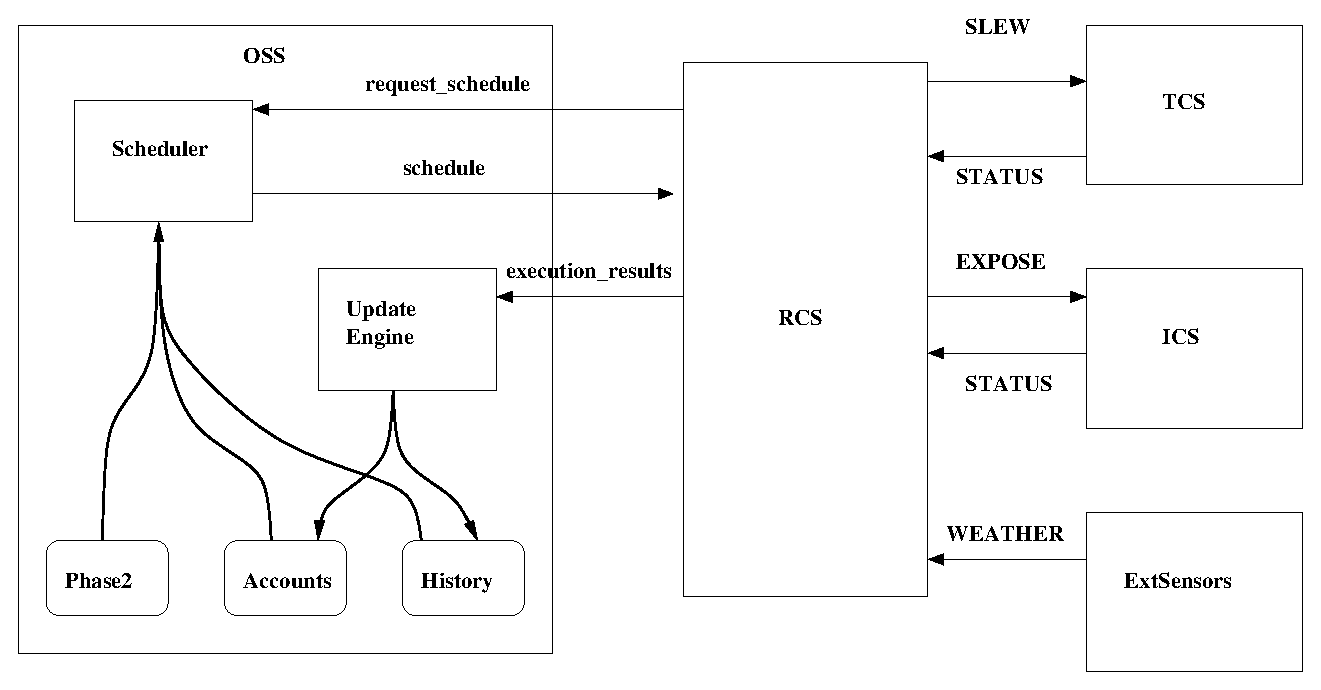
\includegraphics[height=6cm]{figures/overview_architecture.eps}
   \end{center}
  
   \caption[Overview of Architecture.] 
   {Scheduling Engine (SE) uses the Phase2, Accounting and History databases to decide on groups to schedule. On execution of a group the RCS sends results back which are processed by Updating Engine (UE) to update accounting information and QOS Thingy (QT) using group-specific QOS metrics to update history.}
   \label{fig:overview_architecture} 
   \end{figure} 

In the current system the overheads associated with the schedule-execute-update cycle amount to the sum of the schedule generation and instrumentation setup times $t_{sched}$ and $t_{setup}$. This occurs for each cycle i.e. for each group executed. If the group execution time $t_{group} \gg t_{sched}+t_{setup}$ then this is not a great problem. However in the case of groups with short execution times considerable efficiency increases could be achieved by generating a longer schedule sequence with groups chosen so that the setup time between groups is minimized. Real world examples of this scenario have been observed where a pair of short period (in the order of 5 minute) monitoring groups with close targets and with durations of about 2 minutes incurred the full schedule and setup overheads when a pre-defined sequence could have selected the groups to execute in an interleaved fashion with minimal overheads. Another more extreme situation was observed where a single short period monitor was picked to run several times in succession but with the full slew and aquire setup overhead when a pre-defined sequence would have avoided the need to re-aquire the target thus reducing the overhead to almost zero.

\subsection{Research goals}
Quite vague and general - leave details until start of Plan/methodology section after review and before results.

Set the scene and problem statement. Introduce structure of thesis, state contributions 

Reduction of overheads. Flexible schedules. Qos measures. User prefs/metrics, Increase schedule and observation quality. 



% ----------------------------------------------------------------------------------
% REVIEW OF LITERATURE
% ----------------------------------------------------------------------------------
%\chapter{Review of current research}
\section{Review of current research}
Survey and critical assessment. Relation to own work.

Various topics in scheduling literature:-

Online versus offline. Constructive/partial ordered versus iterative,repair based. Flexible schedules.  Search in scheduling. Integrated S+P. Techniques - CSP, agent-based/distributed, evolutionary/bio-inspired/ais, economics/markets, rlt.




 At any point a usable if non-optimal schedule can be extracted by removing unassigned tasks so the technique is applicable in dynamic environments - i.e. reactive repair. NOT TRUE unless we have consistent schedule at that point.


Whichever technique is employed the solution will involve a search over the potentially extremely large space ${D_1 \times D_2 \times \cdots \times D_n}$.  The terrain of this search space can prove be very rugged - \cite{beck97texturebased} have suggested the use of texture based metrics to characterize the structure (short examples)- (and see ref therein to original paper by M. Fox). 

% backtracking for CSPs.
%
\subsection{Constructive techniques}
The constructive approach to generating schedules starts from an empty schedule and progressivly selects tasks to assign to time slots, gradually building up a schedule - effectively a path through the search space. As the search progresses deadend points may be reached when a task becomes unassignable - the search must then backtrack, unwinding pervious assignments and attempting to reassign tasks soas to avoid the deadend. An uninformed search can be very inefficient - if we have $n$ tasks to assign and the domain of each task is of size $d$ then the problem typically is of complexity $O(d^n)$, performance of the search can be improved by using domain knowledge (heuristics) via some of the following techniques:-

\begin{description}
\item[Variable ordering heuristics]
determine the order in which variables are selected for assginment - in scheduling this corresponds to the order tasks are selected for time-slot assignment- e.g. select the task for assignment that leaves the most options left for remaining tasks. The minimum remaining value (MRV) heuristic always selects the variable with the fewest legal assigments to place next - this causes the search to fail fast and allows rapid pruning of the search tree. \cite{sadeh91lookahead} describes a number of variable ordering heuristics used in the MicroBOSS scheduler. These are split into \emph{fixed variable order heuristics} where the order is predetermined at start of search and \emph{dynamic variable order heuristics} where the order is revised each cycle. The \emph{MinimumWidth} heuristic selects the variable with the fewest arcs i.e. constraint associations with other variables. Their \emph{operation resource reliance} (ORR) variable order heuristic selects the task which relies most on the most contended resource or time period The \emph{minconflicts} heuristic \cite{minton92minconflicts} - at each point the heuristic selects a variable that is in conflict and adjusts its value until it is no longer in conflict. Also \emph{maxflex} (myers) and \emph{mincontention} maybe in IR section?) 

\item[Value order heuristics]
determine how the value is chosen to assign to a selected variable. \cite{sadeh91lookahead} describes a \emph{filtered survivable schedules} (FSS) heuristic which assigns to an operation the time-slot which is likely to be compatible with the largest number of survivable schedules = chance of surviving competition with other operations for possession of a resource (time). (Note:simplify the detailed decription in section 6 of the article - concentrate on cliques (clumpings) where graph has tightest constraints = texture heuristics also \cite{beck97texturebased} ). (Note: A couple more examples).They also describe a mechanism to allow the scheduler to switch to a simpler (cheaper) value order heuristics when contention drops below a threshold.

\item[Constraint propagation]
A more general improvement can be made using constraint propagation techniques - here the implications of a constraint on a variable are tested against the constraints on other connected variables. e.g. for arc-consistency there must be a consistent assignment of variables to $X$ for every valid assigment of connected variable $Y$, if not we must delete values from one or other domain. The effects are then propagated to neighboring arcs. The name stems from the way new constraints are inferred and added to the constraints set. $k$-consistency takes this further by insisting that for every $k-1$ assigned variables a consistent value can be assigned to any $k^{th}$ variable. Conflict analysis though costly (typically $O(e^n)$) \cite{muscORpoliORsadeh} can reduce backtracking by pruning the search tree. There is a trade-off in the time taken to perform the consistency checking and the reduction in problem size generated. In \cite{johnston94spike} the use of node ($k=1$), arc ($k=2$)and path ($k=3$) consistency is used to prune the search space for scheduling observations with the Hubble Space Telescope (HST). An example of arc-consistency between binary-constrained variables is given where two observations $A$ and $B$ with a precedence constraint $B$ \emph{after} $A$ by at least $\Delta t$ with each observation having unit duration (for simplicity) and restricted to the interval $[t_A,t_B]$ then the sub-interval $[t_A,t_A+ \Delta t+1]$ is excluded from the domain for $B$ and the subinterval $[t_B-\Delta t-1,t_B]$ is excluded from the domain for $A$. The trade-off in time spent consistency checking against problem reduction is handled in SPIKE by enforcing a strict time-limit for this procedure.

\item[Deadend recovery heuristics] 
The occurance of deadends resulting in the need to perform backtracking indicates that the chosen variable and value ordering heuristics and consistency enforcing technique are insufficent to cope with the problem in hand, a consequence of re-application of these same heuristics on backtracking is that the same deadends may be encountered repeatedly - a thrashing effect similar to that which occurs in disc access. Recovery heuristics are designed to allow for more intelligent choice on how to backtrack. \cite{sadeh94backtracking} describes several general techniques for improving backtracking search using the \emph{partial conflict set} of the deadend (i.e. the set of activities which have blocked progress of the search at that point and which may have been involved in previous deadends):- \begin{inparaenum} \item \emph{Dynamic Consistency Enforcement} (DCE) keeps a history of backtracking events to identify resource critical subproblems and unwinds assignments until a consistent state is reached, \item Learning Order from Failure (LOFF) technique attempts to adjust the variable ordering heuristic on encountering a deadend by unwinding to a consistent state then overriding the default VOH to assign the activities in the partial conflict set before those which would otherwise have been chosen, \item \emph{Incomplete Backjumping Heuristic} (IBH) uses texture based measures \cite{beck97texturebased} to identify assignments which are estimated to lead to more global solutions then when a deadend is detected unwinds to this critical assignment and tries alternatives - e.g. use second best assignment rather than best. \end{inparaenum}

\end{description}

A disadvantage of the constructive approach is its \emph{offline} nature - during execution any break casues the whole schedule from that point onwards to have to be regenerated.




%
% Iterative Repair techniques
%
\subsection{Iterative repair}
Repair based techniques have been a major area in scheduling research over the last xxx years. 

Excellent definition from dejavu scheduler website http://www.dbai.tuwien.ac.at/ proj/DejaVu/document/intro.htm
\begin{quote}
An iterative improvement method is a search method which starts with an initial solution and tries to find better solutions by "local" modifications. The initial schedule can be constructed randomly, by some constructive method, or by a heuristic method. It can also be created by a human or another computer process. To modify given schedules, repair operations are used to transform a schedule into a new and similar schedule. A scheduling operation can be, for example, the exchange of two adjacent jobs, the move of an operation from one resource to another having the same capabilities. If several operations are applicable, a procedure must choose the operation to be applied. This selection can be made randomly or with some look-ahead, allowing to perform the operation leading to the best "neighbor". To determine whether an improvement can be achieved by a operation, the comparison of schedules by an evaluation function must be possible. The most efficient look-ahead is achieved when the schedule evaluation can be determined locally.
A simple hill-climbing algorithm would accept only schedules which evaluate better. Unfortunately, scheduling problems usually have many solutions that differ in their quality, and good solutions are not direct neighbors. Therefore, a search method based on local improvements can be easily trapped in a local optimum. An important feature of all iterative improvement methods is therefore the capability to escape from local optima. However, with this ability, it becomes more likely to search in cycles and some kind of control to avoid repetitions is needed. 
\end{quote}


 Typically operations include \emph{retraction heuristics} used to remove conflicting or oversubscribed tasks or resources and a \emph{repair} or \emph{replacement heuristics} are used to re-insert task(s) at appropriate places. 

\begin{description}
\item[Retraction heuristics] Describe
\item[Repair heiristics] Describe e.g.VarOH and ValuOH
\end{description}

Repair may occur as part of a search process to find an optimal schedule from a preliminary first guess, or may be used in a reactive context to fix an already executing schedule disrupted by unexpected changes to the environment or goals or used opportunistically to take advantage of such changes to increase the global value - e.g. if a task finishes earlier than expected this could provide an opportunity to bring another task forward.

\subsection{Search techniques}
Before embarking on a review of scheduling methodologies we will briefly examine some of the available search techniques which have been applied to scheduling. 

NOTE: Describe what we are searching for - distinguish constructive and repair based - these involve different searches though similar techniques can be employed for both.

Constructive - a path search/route-finding/graph problem.
Repair - searching for a high point on a landscape.

A number of search techniques have been investigated in this field, ranging from mathematical optimization/ constraint satisfaction methods such as Linear and Integer Programming (LP, IP) (REFS eg. H-OPT), local search techniques (Greedy search/hill climbing)(REF), local search with noise (simulated annealing (REF), adaptive noise (REF)) problem-specific (and generic) heuristic methods (MTS, RBDS)(REF), AMP (REF) techniques such as (TABU (REF), scatter search (REF) , A*(REF), LRTA*(REF)), HBSS(REF), SWO(REF), WHISTLING(REF). 

Disinguish local and systematic search (local - neighbourhood, memoryless or small/ systematic - memory, global optimizing) also some notes about representation for constructive and repair based scheduling methods.

A search (or walk) can be characterized by the following basic algorithm: We are moving around in the state space from the current state (schedule assignment) to another selecting a new \emph{successor} state in the \emph{neighbourhood} of the currrent state. The neighbourhood to move to and the successor selection are left to domain-specific or generic heuristics.


\begin{enumerate}  
\item Select initial point $\mathbf{x}$ in the state space (i.e. generate a complete or partial schedule).
\item While time left or goodness criterion not met.
\begin{enumerate}
 \item \emph{select\_successor\_state} (i.e. move to new point $\mathbf{x}'$).
 \item Evaluate objective $F(\mathbf{x}')$ for that point.
 \item If $F(\mathbf{x}') > F(\mathbf{x}_{best})$ then $\mathbf{x}_{best} \rightarrow \mathbf{x}'$
\end{enumerate}
\item Goto 1.
\end{enumerate}



note:
A schedule generated by any offline technique will generally be impossible to follow in dynamic environments for any length of time, and it will have to be re-generated frequently at some cost in time and computing resources.

\begin{description}
\item[Local search]
Moves around current neighbourhood. The various types of local search are characterized by the mechanism for selecting the $move$ operation.

Greedy search also known as hill-climbing and gradient descent is a classic technique. The move operation steps one unit in the direction of highest upward change in objective function - i.e. we move 'up the hill'. The search then proceeds up the local steepest gradient to the peak. This search can become trapped at local maxima, there is no escape to allow the search to explore other parts of the space.

Paper on DTS in ZandF book.

\item[Search with noise]
In an attempt to escape local maxima a number of techniques have been developed to allow a degree of random movement around the search space. HBSS and fukunaga for ASPEN?


\item[Simulated annealing]
(REFS) for this in scheduling context? use decreasing temperature $T$ as search proceeds - probability of random move to low scoring point is $e^{-\frac{\Delta E}{kT}}$. Zweben (anytime rescheduling paper ref? and SPIKE)

\item[Adaptive noise]
As opposed to fixed noise!
This technique is described in paper by \cite{hoos02adaptive}, 

\item[Moving search]
in \cite{yokoo99search} - (MAS/DAI Weiss) here the goals change as we proceed with the search i.e. we are trying to catch a moving target, predator-prey models etc .
Includes MTS and LRTA*. (paper by \cite{ishida96improving} has refs to originals by Korf et al) (Drummond and Bresina RFS paper)

Note: - this is probably more appropriate to DDS later)

\item[AMP]
Adaptive Memory Programming \cite{taillard98adaptive} was first coined as a general term for a class of optimization techniques which use some form of memory to retain knowledge about poor parts of the search space which have been visited recently.

In TABU search \cite{glover99tabu}, as the space around a solution is searched the memory keeps track of bad directions/paths and avoids entering these 'taboo' areas. there is stuff in \cite{xxx} (one of the later nasa papers) about TABU plus SWO and HOPT for spacecraft ops - combined method using IP and heuristics.

In scatter search new \cite{xxx} solutions are generated by evolving solutions in a process similar to that used in Gentic Algorithms (GAs) in that parts of 'fit' solutions are combined to yield new solutions which may be expected to retain some of the 'fitness' of the parents. etc

\end{description}

REfs here to examples of CSP solutions for S+P. Minton - minconflicts heuristic(this can also be in next section!), AMC barrelmaster, SPIKE and HSTS, constraint posting frameworks.
 
\subsection{Case studies}

%\subsection{SPIKE}
Description of SPIKE \cite{johnston94spike}. Initial selection heuristic - \emph{minconflicts}, constraint propagation, repair heuristic(s) etc.
- in the case of SPIKE a conflicting activity is moved to a point where it producues the smallest number of conflicts with other activities. List of quality metrics for good schedule - number of observations, total observing time, summed degree of preference for scheduled observations.

%\subsection{Partially Ordered Schedules (POS)}
\cite{muscettola92bottleneck} describes a system (Conflict Partition scheduling or CPS) for solving scheduling problems by identifying regions of the search space where bottleneck conflicts occur and posting constraints to move the search away from these regions where solutions are unlikely to be found. A bottleneck is defined as a neighbourhood in the search space where the time assignment strategy generates a maximum of inconsistency. These are detected by running a number of stochastic simulations to generate resource allocations with time flexibility. The bottlenecks are identified as those points where the most resource contention occurs and additional sequencing constraints are posted to reduce the contention. They employ two measures of contention - \emph{token demand} $\Delta(\tau,t_i)$ measures how much a token or task $\tau$ relies on a time slot $t_i$ by counting the number of simulations in which $\tau$ was asssigned to $t_i$, \emph{resource contention} $X(\rho,t_j)$ measures how many tokens are competing for a resource $\rho$ at time $t_j$ by counting the number of simulations in which $\rho$ is requested during $t_j$. Simulation uses various variable and value ordering heuristics - FTD, BTD, RVS - DETAILS. Conflict resolution involves - (see their FIG-1 on p5 for algorithm). brief description (esp CPS) - (may not use this list just salient points).
\begin{description}
\item[Capacity analysis]
\item[termination test]
\item[Bottleneck identification]
\item[Conflict identification]
\item[Conflict partition]
\item[Constraint propagation]
\item[Consistency test]
\end{description}

They test against Microboss \cite{sadeh91lookahead} and minconflicts iterative repair \cite{minton92minconflicts}and claim it is better (see the conclusions).


%\subsection{MicroBOSS}
The MicroBOSS scheduler is described in \cite{sadeh91lookahead} - uses lookahead technique (describe) to work out probabilistic demand profile (Section 3 of article) - contention peaks. 

%\subsection{Gerry}
\cite{zweben94scheduling} describe the GERRY system for scheduling space shuttle ground operations. They define 3 types of constraint:- \begin{inparaenum}[(\itshape a\upshape )] \item temporal constraints represent precedneces between activities, \item resource constraints represent usage of resources and \item state constraints represent particular environmental state variable assignments required by some activities - certain activities, denoted as \emph{achievers} are able to set these variables \end{inparaenum}. A weighted penalty function is used to measure the cost of constraint violation. Their repair procedure considers each type of constraint seperately and handles repair of $N$ of each type per cycle before moving onto the next cycle. In order to avoid trapping at local optima in the search space they employ simulated annealing to determine acceptance of a newly generated schedule. At each iteration the cost of the current schedule $s$ is compared to the best so far $s^*$ and is accepted with a probability $P(s,s^*) = \exp{-\frac{|cost(s)-cost(s^*)|}{T}}$ where $T$ is the \emph{annealing temperature} which is cooled during the search. To resolve resource constraints tasks are selected for repair using 3 heuristic criteria \begin{inparaenum}[(\itshape i\upshape )] \item \emph{fitness} - move the task whose resource requirements match the amount of over-allocation most closely - the logic here is that a task which has a small resource requirement is less likely to have much effect, one which has a very large requirement will cause problems wherever it gets moved to, \item \emph{dependency} - move the task which has the fewest temporal dependants - a task with a large number of dependencies will likely cause additional violations when it is moved and disrupt existing assignments, \item \emph{distance} - move the task which needs the smallest move to resolve the conflict - a large move is likely to perturb the overall schedule more. \end{inparaenum}. The results of these metrics are scored and a task selected for the move. State constraints are repaired using a selection of 5 methods in priority order which involve moving the affected task and/or adding \emph{achiever} tasks into the schedule before the affected task to set the variable appropriately. The GERRY scheduler was found to be very effective in the chosen domain and was incorporated into the NASA Ground Processing Scheduling System (GPSS) an interactive tool for scheduling repair and refurbishment of the space shuttles between missions. 


%\subsection{OPIS}
\cite{smith95reactive} describes the OPortunistic Intelligent Scheduler (OPIS) system. This introduces multi-perspective scheduling in which a number of complimentary schedule repair techniques are employed under the supervision of a Top Level Manager (TLM) and working through a common blackboard representation of the current solution and constraints. External events (changes to requirements, feedback from execution) are fed into the blackboard via model update agents. Conflict classes are defined relative to a number of conflict metrics including:- conflict duration, conflict size, resource idle time, upstream slack, projected lateness. A number of agents analyse the conflicts which are then matched to fuzzy behavioural profiles. Schedule repair agents are then selected to apply an appropriate repair heuristic suited to the character of the conflicts. e.g. for a problem with HIGH value of \emph{conflict duration} and LOW value of \emph{variance in projected lateness} coupled with HIGH value of \emph{idle time} the \emph{order-scheduling} heuristic is chosen which revises the sequencing of contiguous operations. In the trade-off between opportunistic improvement and non-disruption to current baseline OPIS is biased towards the later though this is a function of the anaiysis and repair heuristics chosen -- see later under OZONE and DITOPS and AMC papers. (Performance notes...) 

(Note: useful architecture - comaprison to DM concept).

Work on DITOPS \cite{smith96mixed} an air transport scheduler led to the extension of OPIS into a pluggable object oriented framework OZONE (Object Oriented OPIS = $O^3$). This has since been used to implement a number of scheduling systems. .

%\subsection{AMC BarrelMaster} 
For scheduling inflight refueling and transport missions the AMC BarrelMaster scheduler \cite{smith04continuous} was developed using OZONE. In its normal mode of operation the scheduler has to assign times to new missions into an already built schedule. The search strategy \texttt{AssignMission} is based on a triple of:-
\begin{description}
\item[$Gen_{Resources}$] selects candidate resources (aircraft, crew).
\item[$Gen_{Intervals}$] selects candidate intervals for a mission
\item[$Eval_{Criterion}$] ranks alternatives.
\end{description}

The mission requirements generally lead to heavy over-subscription of resources so various relaxation regimes can be considered:- over-allocation of 'reserved' resources, allowable delays, mission combinations, priority pre-emption (bumping). These are handled by selection of different pluggable combinations of these procedures. e.g. $Eval_{criterion}$ has implementations $Eval_{MinTardiness}$ $Eval_{MinFlyingTime}$ and $Eval_{MinOverAllocation}$, similarly there are several versions of $Gen_{Resources}$ and $Gen_{Intervals}$. A procedure \texttt{CombineMissions} allows pairs of missions to be combined to attempt a reduction in resource usage, this can be applied recursively to maximize the reduction in overall flying time required. The primary goal of the AMC Allocator is to assign the most high priority missions, often lower priority missions will be left out even though some assigned high priority missions with greater flexibility are included - an incremental optimization procedure \texttt{MissionSwap} can be applied to try and insert unassigned low priority missions into the schedule by retracting existing commitments and reassigning to free up slots. 

\cite{kramer03maxflex} describe 3 heuristics which can be used to select the tasks for retraction:- \begin{inparaenum}[(\itshape a\upshape)] \item $MaxFlex$ - measures the ratio of required time to available time summed over all resources required by a mission and is an indicator of the flexibility of the mission, \item $MinConflicts$ (\cite{minton92minconflicts}) - measures the number of resource conflicts over a mission's execution interval, \item $MinContention$ - defined as $\frac {\sum_{C \in Conflicts_i} dur_C}{\sum_{r \in R_i ReqInt_{r,i}}}$ where $dur_C$ is the duration of conflict $C$ and $ReqInt_i$ is the required executon interval for mission $i$ measures the proportion of a mission's required interval that is in conflict. \end{inparaenum}. In \cite{kramer04swapping} they extend this technique to minimize disruption to the existing schedule and to speed up the process by search tree pruning. (task pruning - interval pruning - depth bounded search / biased stochastic retraction - VBSS = ACO  - defer to that section or see.Sect. XXX?)...


%\subsection{DITOPS}
DITOPS (Smith and Sycara) based on OZONE.. other paper also under integration of S+P.

in situations of detected constraint conflict an analysis procedure computes a set of metrics, some of which estimate the severity of the problem and some of which characterize the looseness or tightness of time and capacity constraints in the local 'neighbourhood' of the schedule that contains the conflict.


%\subsection{ASPEN/CASPER}
\cite{rabideau99iterative} describes work by NASA JPL on the ASPEN scheduling framework. This is a constraint based search/optimization system intended for spacecraft operations scheduling. During the constraint satisfaction cycle activities are slotted into the schedule and conflicts detected. The system then classifies these conflicts into a large set depending on the type of constraint broken or the type of resource bottleneck. A prioritized sequence of repair heuristics is then selected in turn to attempt a repair which moves closer to satisfycing. (describe algorithm here? or leave to optimizing para).

 ASPEN allows the specification of a number of search heuristics to be slotted in at decision points in the algorithm - some generic ones are described \begin{inparaenum}[(\itshape i\upshape)] \item conflict sorting heuristic (a variable order heuristic)- prefers to repair conflicts which require adding new activities, \item repair selection heuristic - prefers to move an activity then adding activities then deleting activities, \item interval selection heuristic for activities being created or moved (a value order heuristic)- prefers intervals which do not create new conflicts then intervals which minimize new conflicts. \end{inparaenum}.

\cite{rabideau00generic} moves on to describe an extension to ASPEN to allow interleaved repair and optimization using \emph{experts} - these are software components implementing heuristic operations \emph{an expert is a link between changes in the plan and the change in quality}. 

A number of classes of user preferences are defined, some acting on a local level, others globally. These specify a mapping from local variables to scoring metrics - an example given is of a preference on the start time of one activity relative to the preceding one centred on a \emph{preferred} time gap and decreasing monotonically either side within cutoff limits - basically means \emph{I would like a gap of $t^*$ but will be happy with any gap from $t_{low}$ to $t_{high}$} . 

Improvement experts include:- \begin{inparaenum}[(\itshape i\upshape)] \item \emph{local activity variable expert} - considers variables which currently contribute low values to the score - the preferences allow this expert to decide which way the variable has to be adjusted to increase the score (e.g. for the gap preference above, the direction is towards the \emph{preferred} time gap entailing moving one of the activities backward or the other forward), \item \emph{activity/goal count expert} - aims to increase or decrease the number of activities of a given type - the only tactic for this expert is to add or remove activities, \item \emph{resource/state variable expert} - tries to improve the preference scores for resource variables - this can involve moving activities to increase/decrease resource usage (e.g. battery minimum level) or adding and removing activities which increase/decrease the resource level, \item \emph{resource/state change count expert} - is tasked with improving the score for numbers of state or resource changes, \item \emph{state duration expert} - can move, add or delete activities which maintain or cause a particular preferred state. \end{inparaenum}.

In the optimization phase a monotonic increasing assumption is made - i.e. only make (local) changes which will improve globally. A varibale order heuristic selects either the lowest scoring preference or the one with the highest potential gain - $weight_{pref}*(1 - score_{pref})$.

In order to improve overall performance an adaptive noise mechanism following \cite{hoos02adaptive} has been implemented for ASPEN \cite{fukunaga04robust} - this was added to the \emph{repair selection heuristic} above - basically if improvement rate stagnates do some random stuff then after improvement back off but faster $\theta and p$ parameters... XXXresultsXXX and EO-1 application.

The CASPER system \cite{chien99iterative, chien00aspen} was designed as a \emph{soft, realtime} version of ASPEN to act as a framework for dynamic replanning - the concepts of continuous planning, execution and replanning and incremental plan extension. Plan must be continuously modified in light of changing operating context. It advocates a hierarchic system of planning - at higher levels more reasoned plans over long time scales, at lower levels short time scales, more reactive (NOTE: compare Brookes subsumptive architecture).

CASPER's represents the 'world' at a given planning horizon as (current goal set, plan, current exec state, model of predicted states). Updates to any of (goal set, current exec state, horizon (i.e. just time advancing)) causes a replanning iteration - changes are posted, effects propagated - including conflict identification, plan repaired and new working plan results (copy of their FIG7).

\begin{enumerate}
\item Initialize Plan, Goal-set, State.
\item Update G to reflect new goals and remove spurious.
\item Update S to current execution state.
\item Compute conflicts.
\item Apply conflict resolution to generate new Plan.
\item Release for execution.
\item goto 1.
\end{enumerate}

\cite{chien98integrated}, Benefits -(responsiveness to sudden changes in environment, predictive modelling errors reduced due to continuous updating, fault protection moved from exec layers working on very short time scales, reduced distinction between PSE due to layering??). Currently the system can only replan at activity boundaries - unable to model effects of interrupted activities. Extension to include (plugin) goal achievement modules (GAMs) - experts at solving specific types of conflict - e.g. spacecraft attitude conflicts - XXXlook for newer paper on these- context DS-4XXX


XXXDetails of some NASA application areasXXX.

%
% Contingent methods + constraint posting
%
\subsection{Contingency and flexibility methods}

What can go wrong - new tasks arrive, resources fail (e.g. instruments offline),

Motivation - localize changes, make them small, continuity of \emph{global plan}, reactive repair must be fast. 

Approaches - contingency - build multiple futures, execution branches to cope with what might happen. 

Different approaches \cite{policella03flexible} classifies these as:-

\begin{description}
\item[Robust solution] create a robust schedule with built in flexibility (time slop).
\item[Partially defined schedules] Define partial order of activities.
\item[Rescheduling] as already discussed.
\item[Dynamic] Despatch scheduling.
\end{description}

Examples (Muscettola+Smith /HSTS, Sadeh/MICROBOSS), (Bresina et al/JIC), SPIKE others.

\cite{davenport01slack} compare 3 pro-active techniques for building extra time into a schedule to cope with uncertain duration. \emph{Temporal protection} adds a slack time into each activity duration prior to the search, \emph{time slack window} uses reasoning during the search to attach minimum slack into each activity, \emph{focused time window slack} (FTWS) assigns slack based on the distance along the planning horizon. Normal distributions  are used to model the likelihood (MTBF) $N(\mu_{tbf}, \sigma_{tbf})$ and length (downtime) $N(\mu_{dt}, \sigma_{dt})$ of breakdowns:-
\begin{eqnarray}
slack_A(t) & >= & \sum_{n=1}^M P(N(\mu(n),\sigma(n)) <= t)  \mu_{dt} \\
\mu(n) & = & (n \mu_{tbf}) + ((n-1) \mu_{dt}) \\
\sigma(n) & = & \sqrt{((n \sigma_{tbf}^2) + ((n-1) \sigma_{dt}^2)}
\end{eqnarray}
where $\mu(n)$ is the mean value of the probability of $n$ breakdowns of the executor and $\sigma(n)$ is its standard deviation. When tested on simulated problems with varying degrees of uncertainty (breakdowns) all methods help improve tardiness with increasing degrees of uncertainty. They do not however give account of the tradeoff due to uneccessary slack time introduced by the technique relative to the gains of continuity and reduced need for rescheduling.


Two different approaches are compared by \cite{policella03flexible} (WHAT CONTEXT) and described in more detail \cite{policella05thesis} 
They define 3 measures of robustness - \begin{inparaenum}[(\itshape a\upshape )]\item reactiveness - speed of response, \item stability - degree of change induced by reaction - ripple effect, \item solution quality - preservation (or enhancement) of performance relative to baseline schedule.\end{inparaenum}. Two metrics are defined for evaluating schedule quality:-
$fldt = \sum_{i=1} \sum_{j \neq i} \frac { |d(e_i,s_j) - d(s_j, e_i)|}{ H \times N \times (N-1)}$
where $d(x,y)$ is the distance between $x$ and $y$ and $e_i$ is the finish time for activity $i$ and $s_i$ is its start time. This metric is designed to evaluate the fluidity of the schedule i.e. its ability to absorb time variations. Small values of $fldt$ imply that effects will be localized rather than ripple through the schedule. The second metric:-

$dsrp = \frac{1}{n}\sum_{i=1}^{n} P_{dis}(a_i) \frac{slack_i}{num_{changes}(a_i, \Delta a_i)}$
where $slack_i$ is the slack available to activity $i$ and $num_{changes}(x,y)$ is the number of activities moved from their start times when activity $x$ is delayed by $y$ with $P_{dis}(a_i)$ estimated as $\frac {duration_i}{makespan}$ discribes disruptibility of the schedule and they claim it measures \emph{the price to pay for the flexibility of the schedule}

The first technique \emph{resource envelope based} employs a 2 step process. 
In the first step, from an initial partially ordered schedule with constraints they compute the resource-envelope (a time varying measure of resource requirements), using this they then detect conflicts (where more activities require a resource than its capacity allows), a selection heuristic is used to rank and then select a pair of competing activities, a sequencing heuristic then specifies (posts) new precedence constraints to remove this conflict. The resulting modified schedule with new constraints is fed back into the first step until a solution is found.
The second technique \emph{earliest start time} starts with a pre-selected fixed-time schedule, then selecting activities based on ranked order of start times and using a cheaper resource analysis posts new precedence constraints which can be used to determine the bounds for eachactivity to prodcuce a flexible schedule. They find that the second approach perfoms best against all quality measures and is fastest.  

In \cite{muscettola92bottleneck} Conflict Partition Scheduling (CPS) in context of HSTS - partitioning of bottlenecks 
uses constraint posting and stochastic simulation to locate areas of search space where solutions are unlikely to be found. MOVEBACK

In \cite{sadeh91lookahead} the /MICROBOSS scheduler - lookahead techniques, aggregate demand profile, ORR and FSS (already mentioned) - ONLY IN INTRO

\cite{bresina94jic} take a different approach (JIC) to a scheduling problem involving selection of observations for the XXX telescope in which the main source of uncertainty relates to the lengths of observations (action duration uncertainty). Uncertainty is due to star-centring which depends on sky conditions, wind, pointing etc. Uncertainty grows with time. Online scheduling is slow (whole night's observations to allocate to enablement intervals). 


They run multiple simulations over the night looking for the most likely break points then look for alternative branches to execute... details also \cite{drummond94jic}.

\begin{enumerate}
\item Estimate temporal uncertainty at each activity point.
\item Find most probably breakpoint.
\item Create branch (do X or nodo X).
\item Reschedule subproblem (doall before X, nodo X)
\item Integrate with prior schedule.
\item repeat goto 1 while time left.
\end{enumerate}

Hard to explain without diagram..worth reproducing their FIG 1 and adding some notes.


 Problem is to create a multiply contingent schedule from a fixed schedule in a reasonable time soas to increase robustness. Large search space if any action can break - need to reduce number of branch points to manageable size. 

 Improved for Mars rover \cite{bresina99increased} additional resource uncertainty not just time, expected utility to select branch not just p(fail), allow setup steps prior to branch point.

and note use of HBSS \cite{bresina96hbss}.
 
%
% Integrated Planning and scheduling
%
\subsection{Integrated Planning and scheduling}
Discuss attempts to integrate the 2 - including dynamic planning - CPEF 
Refs - (Myers, Smith, ) \cite{chien98integrated}

\cite{myers01integrating} 




% Reactive scheduling.
\subsection{Reactive scheduling}
Discuss examples or RS and DS .

Reactive scheduling deals with the repair of executing schedules which have become inconsistant or broken due to changes in the environment. If the goals (objectives) are changed dynamicaly, an executing schedule may break or become sub-optimal, reactive scheduling deals with this situation also. A subclass of reactive scheduling is dynamic scheduling (see \ref{sect:dynamic}), where the decision of what to schedule next is made at that point in time - there is no look-ahead though the history of the execution to date may be available.

\cite{jones98survey} describes 2 classes of reactive system:-
\begin{itemize}
\item reactive repair - the system waits for an event to occur before attempting to recover the system.
\item in pro-active adjustment the system monitors continuously, predicting the future evolution and attempting to plan ahead for contingencies while the plan is executing.
\end{itemize}

% Dynamic despatch scheduling.
\subsection{Dynamic Despatch scheduling}
\label{sect:dynamic}
Standard DS/QueueT algorithms (Karaman A, survey paper?)  Priority rules = (EDD, SPT, MinSlack, etc)

Uses of DS (LT original papers).

Paper by (Shaw and Raman) about use of machine learning to induce despatching rules (CBR).

DESCRIBE SEU cycle, pools, priority rules, queues and other general stuff- esp wrt current project.

%
% Agent based scheduling.
%
\subsection{Agent based scheduling}
Various papers. 

%
% Evolutionary and biologically inspired techniques applied to scheduling 
% e.g. swarms, ACO, Wasps.
%
\subsection{Evolutionary and biologically inspired techniques}
e.g. GAs, swarms, Ant Colony Optimization (ACO), Wasps (Whistling algorithm), artificial immune systems (AIS).

Genetic Algorithms (GA) are described by \cite{russel03artificial} as a form of stochastic hill-climbing search with random exploration and exchange of information between parallel search threads. (Examples of use in S+P).

AIS (Hart99 +other, and refd in Kocjan02).


%
% Reinforced Learning techniques applied to scheduling.
% TD(lambda), Q-learning, MDPs.
%
\subsection{Adaptive Learning techniques applied to scheduling}
Papers by (Riedmuller etc). Discuss briefly TD($\lambda$), Q-learning, MDPs.

Reinforcement learning techniques involve learning policies for state-space problem solving. For each state $s \in S$ the policy $\pi:s \rightarrow a$ determines the action $a \in A$ to perform. While learning, the system receives a reinforcement signal or reward after each action. The goal is to find an optimal policy $\pi^*$ which maximizes the expected cumulative reward over future action. In scheduling, the policy tells us how (what scheduling action to perform) to maximize some measure of schedule quality in the final realized schedule.

Motivated by the myopism of local despatching rules which lead to supboptimal global behaviour, \cite{riedmiller99neural} have studied the use of RL techniques to learn despatching rules which adapt dynamically using feedback from the evolving problem situation. The problem is represented as an MDP where $s(t)$ represents the allocation of tasks to resources at time $t$ and $a(t)$ represents the selection of the next job to allocate. Individual Q-learning agents with local state and action knowledge are associated with each resource. They used an MLP to represent the value function, taking as inputs a number of problem features culled from the problem space (set of unallocated tasks). These include features relating to the current schedule state:- tightness with respect to due dates, estimated tardiness, estimated makespan, average slack, and features dependant on the next job selection such as:- average remaining slack if $job_i$ is selected, relative slack ($job_i/total$). By varying the set of input features selected to match those of standard despatch heuristics (EDD, SPT, LPT, FIFO, MinSlack) they were able to train the network to produce despatch policies which met or exceeded the performance of these heuristics on problems to which the specific heuristics were best suited. By combining sets of input features they were also able to outperform all of these despatch heuristics on a variety of problems. In effect the network was able to learn better policies by combining the standard heuristics depending on the problem features. When applied to untrained problems the network was able to successfully generalize and improved significantly on each of the standard despatch policies.

Though possible to engineer domain-specific heuristics by hand to exploit regularities and features of a problem space, this can be time consuming and expensive and is naturally non-general. This was the motivation for \cite{zhang95reinforcement} who have studied the use of RL techniques to learn heuristics. Using a $TD(\lambda)$ based technique in which the value function is represented by the weights in a feed-forward network, the reward at each learning step $t$ is computed as the summed relative utilization index (RUI) for each resource at that time step (latex doesnt like this eqn so left out for now).


\begin{equation}
RUI_i(t) = 
\begin{cases}
1& \text{$U_i(t) < c_i(t)$} \\
U_i(t)/c_i(t)& \text{$U_i(t) >= c_i(t)$}
\end{cases}
\end{equation}
%% ONE DAY THIS EQN WILL WORK AND ALL WILL BE WELL


Their system models an iterative repair technique. The states represent the constructed schedule at a point in a sequence of repairs to obtain an optimal schedule and the actions are selected from a set of repair operations. They use a number of features extracted from the partial schedule at each learning step as inputs to the NN and this is used to estimate the value function. In tests against an iterative repair technique empolying stochastic search via SA \cite{zweben94scheduling} the system was able to learn a repair policy after training which beat the IR technique consistently for speed though the IR technique was able to produce better schedules given sufficient time.


In dynamic systems \cite{shaw90intelligent} hypothesise that the rules used to make scheduling decisions should change with time as the problem characteristics evolve. They proposed a system which distinguishes between and ranks problem characteristics by relative importance, then performs adaptive scheduling by opportunistically selecting appropriate heuristics. 

The system called Pattern Directed Scheduling (PDS) works in 2 stages. In the first step (learning stage) a series of training scenarios are simulated and used to study the effects of applying various despatching rules. A critic module (the expert) analyses the performance of these rules on the problem scenarios and may generate new training examples to refine the matching of patterns to rules. The system chosen for induction was based on Iterative Dichotomizer 3 ID3 \cite{quinlan86induction}, in this system a tree of rules is built up by splitting the domains of the problem attributes (summary explanation in Hopgood KBS for E and S). 

An effect of this system is that it ranks the attributes in terms of an entropy - \emph{how much does attribute $j$ contribute to the knowledge used to make a given decision ?}. This has the advantage of allowing us to see which attributes are important and which are irrelevant or decision-neutral but does have the disadvantage of considering each attribute in isolation and is unable to detect interdependancies between attributes. A typical example being where a decision should be made based on the similarity of 2 attributes rather than their individual values. Shaw et al used a total of 9 problem attributes and found that 2 of these were irrelevant. 

They found that when applying the learnt rules to real problems it was important to reduce the \emph{nervousness} of the system. As the characteristics changed it was neccessary introduce a smoothing component to avoid switching rules too quickly by waiting until the selection count of a new rule had reached a threshold value. They tested the system against a number of standard despatching rules with a collection of problem instances and concluded that there was an overall improvement of around 11.5\% in mean tardiness compared to the best of the single rules applied to any of the problem sets. The improvement was atrributed to the adaptive selection of rules and the ability to use feedback to refine the heuristic selection.


Case based reasoning (CBR) is a learning technique in which rules are induced by matching problem situations against a set of examples (the cases). It has several advantages:- CBR is particularly useful at extracting rules from noisy data, it operates incrementally building up its knowledge base while working (there is no large expenditure of effort at the start of the process or any need to check consistency between rules as in a rule-based learning), contextual information may be retained in the cases to help human assessors to understand the induced rules.

Due to their interactions and conflicts, it is often difficult to determine numerically or in terms of hard-and-fast rules, the relative ranking and trade-offs between users' schedule optimization preferences. The CABINS system \cite{miyashita95cabins} uses CBR to capture these preferences. CABINS provides a framework for acquiring preferences then uses the case base to improve schedules and provide a reactive repair mechanism in response to unforseen events. 

The system operates in 2 stages:-
\begin{enumerate}
\item In the first stage,a feasible but sub-optimal schedule is generated using a constructive technique. 
\item In the second stage the schedule is improved by selecting repair actions (iterative repair). The quality of the schedule before and after each repair are compared using a number of local (pertaining to the current \emph{focal} activity) and global (referring to the overall schedule) criteria (e.g. tardiness, WIP inventory, waiting time...). Repair operations are interleaved with consistency enforcment - as a repair on the currently selected \emph{focal} activity is made it is likely that constraints may be broken requiring other activities (conflict set) to be rescheduled. 

CABINS has 3 operating modes:-
\begin{itemize}
\item In \emph{knowledge acquisition} mode the user selects the repair actions to perform and these decisions are stored along with information to characterize the current problem situation (a case). If sufficient training examples are provided, the resulting case base should contain a distribution of examples covering a diverse set of problem situations.

\item In \emph{decision support} mode, the system selects repair actions by matching the current problem to the repair actions in the case base and an interactive user has the option to veto/override providing additional training.

\item In \emph{automatic} mode, the system makes all repair decisions using the case base without user interaction.
\end{itemize}
\end{enumerate}

Selection of repair actions is performed by matching the problem profile against the stored cases using a $k$-nearest neighbour matching algorithm:-
\begin{eqnarray}
distance_i = \sum_j (salience^i_j (\frac {CaseFeature^i_j - ProblemFeature_j}{E_{dev_j}}))^2 \\
similarity_i = \exp^{-distance_i}
\end{eqnarray}
where $salience^i_j$ represents the user's evaluation of the importance of case feature $j$ of case $i$, $CaseFeature^i_j$ is the value of feature $j$ of case $i$, $ProblemFeature_j$ is the value of feature $j$ in the current problem and 
$E_{dev_j}$ is the standard deviation of feature $j$ for all cases. $distance_i$ is the dissimilarity between the current problem and the $i^{th}$ case and $similarity_i$ is the similarity between the current problem and the $i^{th}$ case.

The repair process operates as follows:-
\begin{enumerate}
\item A focal activity is selected and a start time predicted using each of the available tactics.
\item The conflict set is worked out by projecting the (ripple) effects of the repair onto neighbouring activities.
\item Consistency enforcement technique works on the conflict set using the Activity Resource Reliance (ARR) variable ordering heuristic which selects the most critical activity (most likely to be involved in a capacity conflict over the repair horizon) and a greedy value ordering heuristic which selects a time assignment for the selected activity according to a bias function which represents the time-varing utility perceived for the activity start time deduced from the case base.
\item The activity utility functions are updated - they are biased to start times calculated as part of step (3) to be used in the next iteration.
\item CBR is used to evaluate the quality of the new schedule.
\end{enumerate}
They performed a series of comparisons against other methods evaluated against teh following criteria: \begin{inparaenum}[(\itshape a\upshape )] \item attendance to scheduling objectives, \item amount of disruption, \item efficiency (speed) - especially in respect of its use for reactive repair \end{inparaenum}.

Compared with SA based IR scheduler. Found that ~1000 cases was optimum - marginal improvment above 1000 was not worth the effort. They concluded that CABINS was good at capturing preferences and optimization trade-offs that are difficult to model, improved schedule quality irrespectively of how the initial (seed) schedule was generated and produced high quality schedules faster than simliar IR technique so was suitable for reactive scheduling.


NOTE (need to read that paper again as the repair/CBS intervleaving technique does not seem quite right.

\cite{sycara96case} extended the CABINs framework to consider time-varying user preferences. Their extension allowed the system to learn new cases from its own evaluations of schedule improvment while running. They employed a \emph{rolling horizon} model in which the matching algorithm gives more weight to recent cases than to older cases.

Some techniques involving learning despatch rules/priority weights GEN-H \cite{morris97automatic}. 


%
% Economics and market based techniques applied to scheduling.
%
\subsection{Economics and market based techniques}
Various papers.

%
% Telescope specific scheduling
%
\subsection{Telescope domain}
Examples - SPIKE (already done), APA, ...


\include{plan}

% May be split.



% ----------------------------------------------------------------------------------
% ANALYSIS, DESIGN, IMPLEMENTATION AND RESULTS OF PROJECT
% ----------------------------------------------------------------------------------

\section{Plan}
In this bit describe what the whole project is about and how things will be done
-experimental methods 
\begin{enumerate}
\item Investigate metrics with which to compare the efficiency and quality of generated schedules.
\item Design software instrumentation to embed within the current robotic control system to collect data with which to characterize the operating environment.
\item Using data collected by the embedded software, I will design a simulation framework incorporating knowledge of the operating environment characteristics with which to test any schedulers developed.
\item Develop a despatch scheduler as a baseline with which to test more advanced schedulers, this will be capable of configuration to use different scheduling policies.
\item Tune the baseline scheduler using various controllable parameters, typically objective weighting functions and biad function, to investigate the limits of this scheduling paradigm in the telescope scheduling context.
\item As the basis for the final system, I will develop a look-ahead scheduler incorporating short-term prediction of environmental statistics to allow advanced planning of observations and using feedback of performance to adjust the plan objectives.
\item Investigate variation of scheduling control parameters and horizon length on quality of schedules generated under varying environmental models to determine how to adapt to these - teh quality of schedules generated will be compared to those geenrated by the baseline system working at its maximum efficiency.
\item Knowledge gained from this investigation will be incorporated into a final adaptive, look-ahead scheduler.
\end{enumerate}

Some more details on plan...
\begin{enumerate}
\item Develop metrics. Global quality to compare policies and architecure, local within arch to guide search.
\item Data gathering - statistics of environment, P2DB characterization and rate of change.
\item Develop scheduler.
\item Prediction of environment and other models - test.
\item Forward planning i.e. lookahead and predicted reward of future actions.
\item Compare local despatch to expected future rewards model.  (m/c sims). \cite{bresina95expected} has excellent discussion on this topic wrt ATIS.
\item Variation of weights and (search) metrics.
\item Compare effects of various stochastic bias fns.
\item Distributed scheduling architecture - take into account user/group preferences (DMs).
\item Global optimization of DSA/DM.

\end{enumerate}

How does this manifest itself wrt actual studies/experiments ?
\begin{enumerate}
\item Metrics investigation study (Sect. \ref{sect:metrics_study}).
\item Database characterization study (Sect. \ref{sect:db_character_study}).
\item Data collection and prediction study (Sect. \ref{sect:prediction}).
\item Scheduler architecture and simulation framework study (Sect. \ref{sect:sched_comp_study}).
\item Case study 1. 1 or 2 night shakedown, effects of $w_p$ and $w_t$ (Sect. \ref{sect:cs1_study}).
\item Man against machine study (Sect. \ref{sect:mam_study}).
\item Long term case study. Many scoring and selection options, tracers (sect. \ref{sect:lts_study}).
\item Advanced architecture and framework enhancements.
\item Long term case study 2. Advanced LAS/BAS extract SQM under varing conditions.
\item Long term case study 3. LAS/BAS adaptation to predicted conditions.
\end{enumerate}

Note: Data collection: If running a simulation over an extended period, the DB content would naturally change, need to be able to gather P2DB arrival and modification statistics - i.e. want to know how the DB changes in time not just a snapshot at T - this cant be very detailed just how many groups added/removed - maybe some statistical data could be extracted on a daily basis from P2DB e.g. average exposure length, spread of group lengths - needs more thought - this is a means of characterizing the DB - can then generate simulated datasets in addition to snapshots of real data. 




% PART II Studies/Experiments
\section{Investigation of Metrics}
\label{sect:metrics_study}
An investigation into possible metrics for determination of schedule quality.

\subsection{Introduction and rationale}
Metrics - basically quantative standards for measuring performance, quality or some aspect of a service or process we wish to monitor. In the context of scheduling these can be broadly divided into problem complexity metrics and schedule quality metrics. Problem complexity metrics (PCM) measure the difficulty of a scheduling problem and provide an independant variable with which to asses the performance of schedulers. It might be found for example that a particular scheduler which performs well on a \emph{easy} problems is out-performed by an alternative scheduler when faced with \emph{difficult} problems. Schedule quality metrics (SQM) measure the actual performance of schedulers on such problems - this in essence is what the whole project is about - the determination of the best scheduler under given conditions. A third set of metrics which will not be discussed in this section are those metrics used by the actual schedulers to perform scoring, selection, retraction and other heuristic procedures in the determination of schedules - these will be discussed in the relevant scheduler descriptions (Sect. \ref{ss:schedulers}. (XXX)

% NOTE this is a reference to one or more sections in the schedcomparch/scoringmodel etc  and future schedulers on the 
%      items used to make the thing work.

\subsection{Problem complexity metrics (PCM)}
\label{ss:pcm}
These metrics describe the complexity of the scheduling problem at any given time. In addition to there use for assessing the performance of schedulers under test, it is likely that an advanced scheduler could itself make use of these metrics by looking ahead to see where hotspots (difficult scheduling periods) are likely to occur and thus take these into account in its decision making - this would introduce a feedback effect which would make the whole exercise rather more as the degree of feedback ought to be determined and taken into account in any complexity assessment.


 The basic problem is to schedule the observations in the ODB, consequently this is where the focus of the investigation begins. The content of the observing database or pool (ODB) at any time defines the set of observations that are available for scheduling at that time. This pool evolves due to the arrival of new observing requests, modification of existing request (e.g. in light of observing results) and removal of spent requests. These modifications which may be made by observers themselves via a phase2 tool or automatically by external user agents occur in principle continuously. The complexity manifests itself through changes in the amount and severity of competition between observing requests for particular times and over the course of a night in the overall load.

These metrics will be denoted hereforth using the notation $C_x$ to indicate a \underline{c}omplexity metric with subscript, here (x) to denote a specific aspect.


\subsubsection{Contention profile $C_c$}
This is the time evolving profile of the number of observation groups which could be scheduled according to their explicit timing constraints. Additional refinements include convolving with the probability of the time actually being available based on likely weather and technical downtime forecasts. The average contention over the course of a night gives an estimate of how overloaded the schedule could potentially be. This static contention profile is a crude measure as it does not take into account the fact that some of the groups which figure in the contention profile later in the night may have already been selected by then and thus need not be considered. Another possibility is to introduce a weighted probability of execution on those groups figuring later in the night to reduce the the effect of early executions, - e.g. a simple exponential decay from $P_{avail}=1$ at the start of group's execution window with decay factor based on the group's likely execution - though how do I work that out ? - most likely this would depend on the contention statistics we are actually trying to work out ! Effects of disruptors early in the night will also change the contention later as groups which \emph{ought} to have been executed may still be in contention later. The dynamic contention profile $C_c$ is calculated by performing a forward simulation through the night and extracting actual contention in the process - this is of course somewhat dependant on the scheduler used but can be a valuable tool for assessing the degree of competition between groups

\subsubsection{Demand profile $C_d$}
A given group will potentially have multiple observing windows when it should be attempted. During any given window the group can be considered to have a demand D on the time within that window. E.g. if the group $g$ has an (estimated) execution time $X(g)$ and its window of opportunity is $\phi(g)$ \footnote[1]{this is the window during which it may legally start, it may run on over the end of the window as this is taken account of in determining whether the group could be executed} then the group's demand over that window is $D=X/(X+\phi)$. If we add up the demand contributions of all the groups which are enabled at any given time we should have a measure of how much demand is placed on that instant. If this aggregate demand exceeds unity then it is likely that some of the groups will not be observed i.e. the requirement for time is greater than the time available. 
There are several refinements that can be made on this estimate. Firstly we can work out the numerator fairly easily - it can usually be considered constant and known. The denominator is more of a problem. Firstly working out the window of opportunity from the group's time constraint window \textsf{W} is straightforward, however this window may extend from just a few minutes upto several days or even weeks. In the later case the group's target(s) may rise and set several times and the various implicit timing constraints may be broken on several occasions e.g. the lunar distance constraint will impose a varying overlap with the target visibility windows. If we consider each of the calculable constraints then we can work out the actual amount of time (within the window) that the group can
actually be observed - this gives us a revised (increased) estimate for the group's individual demand for those times within the new sub-windows. 
Going on another stage we might consider those constraints which cannot be worked out in advance. A group may have a minimum seeing constraint - we cannot tell what the seeing will be like at any future time though we may be able to estimate the likeliness of attaining the group's minimum level. Likewise we can obtain estimates of extinction (perhaps including seasonal variation). We should in addition consider the probability that the selected time is even available for observing - weather and technical downtime mean that a certain fraction of time is lost - a crude climatological estimate might just give the average probability of bad weather (averaged over long periods), we might also have more accurate seasonal-adjusted climatological information, better still if we can predict for some time ahead based on current and recently collected weather data then we shall have a better demand estimate i.e. we are calculating the likely time available rather than the certain time available for the group.

Formally:- Let $X(g)$ represent the \emph{estimated} execution time of a group $g$ and $U(g,t)$ the remaining useful time left for that group at time $t$, then the partial demand of $g$ at time $t$ is defined as:

$d(g,t) = X(g)/(X(g) + U(g,t))$ where $U(g,t) = \tau(w^*_i) \cap [t,\infty] \cap N(t) \cap M(g) \cap V(g))$ and others, where $V(g)$ is the set of visibility windows for $g$'s targets from $t$ onwards, $M(g)$ is the set of windows satisfying observing constraints, $N(t)$ the set of nights from $t$ onwards.

Some stuff on seeing/extinction stats. More on weather/technical downtime.

If a group $g$ is to execute at some future time $t$ we need to know that the weather will be good at that time and that it will remain good for at least $X(g)$. From the weather stats:- 

$P_{exec}=P_{good}(t) \dot \int_{t=X(g)}^{t=\infty}{\rho(t)dt}$ where $\rho(t)$ represents the distribution of lengths of continuous \emph{good} weather runs.

\subsubsection{Load $C_l$}
The load is a fairly simple metric which describes the ratio of executable time in a given observing night to the length of the night (or astronomical night). Simple load is calculated using the sum of execution times for each executable window of each group that can be executed during the night. It includes all windows of all groups whether they \emph{must} be executed that night or not. An urgency weighted load $C_{ul}$ can also be calculated which weights each execution time by the reciprocal of the number of remaining nights in which the window could be observed. Critical load $C_{cl}$ is a pruned version of the normal load where only groups which {\bf must} be executed that particular night are included. Priority weighted load $C_{pl}$ is calculated by taking into account all of the groups' windows which \emph{should} be executed on a given observing night (as opposed to those groups which \emph{might} be executed. The sum of execution times for each window is weighted by the priority of the group whose window it is. This is in effect the potential maximum value for the $Q_{PX}$ SQM and can be used to normalize this.

\subsection{Schedule quality metrics (SQM)}

These are the metrics used to compare the results of using different schedulers or scheduling policies on a given scheduling problem. These are needed to determine which scheduler performs best. Needless to say this is the most difficult problem for several reasons.
\begin{itemize}
\item The metric used in the selection heuristic cannot be used for the simple reason that these may be what distinguishes one scheduler from another - clearly if we use a metric $m_1$ for scheduler \emph{S\_1} and metric $m_2$ for scheduler \emph{S\_2} then measuring the performance of both schedulers using $m_1$ would naturally find that \emph{S\_1} was the better scheduler. Likewise using $m_2$ to compare the results would reveal \emph{S\_2} as the better scheduler. We therefore need a more generic metric which is ideally {\bf NOT} involved in the selection process.
\item What was that other one ?
\end{itemize}

This turns out to be particularly difficult. In the common scheduling literature there are many generic metrics used, however these all suffer from the problem that they are tuned for the generic job-shop scheduling problem in which a number of identical jobs with specified due dates have to be processed. Typical metrics include:-

\begin{itemize}
\item Slack - the amount of time where no job is in progress.
\item Tardiness - total lateness for jobs executed.
\item Throughput - total no of jobs through the system.
\item other
\end{itemize}

Can we use any of these ? The problem is that the OGs generally have a due dates which cannot be exceded - if they are late the data is of less or no use. We are not neccessarily bothered about throughput so much as the quality of the results. 

we might be able to use some of this however with suitable weighting e.g. a late high priority job is worse than a late low priority job (but by how much?). 

We can seperate out various forms of utility measure (NOTE these are discussed elsewhere but not in correct place)

User based (needs simple Phase2 specification or QOS metrics)
Enterprise based - includes scientific priorities, distribution of time between proposals.

\subsubsection{Potential utility measure} Work out the best utility that can be achieved during the night (PU) (i.e. assume we can do all the groups that could be done and do them at the best possible times) - this is after all the ultimate aim of the scheduler ! Work out the actual utility scored by the scheduler that night - the Efficiency (E) is then the ratio. May need to scale - after all if oversubscribed we could never do it all anyway try load scaling 1/L (load defined as aggregate (average) demand) or maybe better as \emph{sum of execution times of all groups that can and {\bf should} be executed tonight}. Could also try rank-scaling top(n) such that $\sum{x_i} < \tau(n)$ - I cant quite recall what I meant by that at the moment.


\subsubsection{Primitive utility measures}
There are a number of primitive measures that could be used independantly - in reality the complex tradeoffs between these make a more generic measure more useful however there is likely still some value in using these. These measures are by and large \emph{single night} measures. 

\begin{itemize}
\item Height metric $Q_H$ measures the difference between the optimum time for performing a group based on its height to transit height ratio during the night and its actual selected execution time. By adding these up we get a measure of badness - i.e. ideally all groups would get done at their highest point (in the feasibility window).

\item Optimal Height metric $Q_{OH}$ measures how close to the \emph{optimum} height the group is observed in its execution window. 

The optimum height is basically the highest elevation attained by the group during the feasible observation window - in a given window this may be at the end (rising target), start (setting target) or somewhere in the middle of the observing window (transiting target). 

There is however a non-linear relationship between elevation and airmass such that for targets which do not rise particularly high the difference in image quality between worst and best case elevation may be high over a relatively small elevation difference whereas for high rising targets the difference in airmass and hence image quality between best and worst case elevations will be small for the same elevation difference .



Consequently it may be better to measure the ratio of execution-time airmass $a_{actual}$ to best achievable airmass $a_{opt}$ as an Optimal Airmass metric $Q_{OA}$. 

Additionally, the \emph{benefit} (image quality advantage) of one airmass over another may itself be non-linear and this is what we should really be measuring. $Q_{BA}$ measures the ratio of some decreasing benefit function $b(a)$ of airmass $a$ at optimal airmass and actual execution-time airmass. A simple option for $b(a)$ would be to use the known correction  \cite{standard airmass/wavelength correction paper} of image FWHM or seeing $s$ for airmass relative to \emph{ideal} seeing at elevation $90^\circ$, $s(a)=s_{90}a^{0.6}$ with $s_{90}$ indicating the image FWHM at $z=0,a=1$ and assuming image quality is judged purely (and linearly) on FWHM. It should be noted that this correction depends also on observation wavelength $\lambda$. Figure \ref{fig:baz_plot} shows 2 models for $b(a)$ based on the standard FWHM correction.
\begin{equation}
Q_{OA} = \frac{1}{L(S)}\sum_{g \in S}{\frac{a_{opt}}{a_{actual}}}
\end{equation}
where $a = \sec{z}$ is the airmass of group's target at zenith distance $z$.

\begin{equation}
Q_{BA} = \frac{1}{L(S)}\sum_{g \in S}{\frac{b(a_{actual})}{b(a_{opt})}}
\end{equation}
where $b(a)$ represents the benefit (image quality advantage) for airmass $a$.

\item Monitor window metric $Q_{MW}$ measures the difference between the optimum time (wrt the centre of a monitor window) for performing a group based on the known monitor window and its actual selected execution time By adding these up we get a measure of badness - i.e. ideally all groups would get done at the centre of the monitor window. (there are some implications wrt non-monitor groups - how do we select the centre of the window ?. What if the window centre is not actually feasible - how is this taken into account  - do we pick nearest feasible point in window either before or after centre  - can also do something like $u(t)$ = some function which peaks at the window centre and we want the group done at t where $max_{t \in \textsf{W} \cap \textsf{T}}(U(t))$.   

\item Priority metric $Q_{PX}$ measures the total priority score achieved i.e just sums up the priorites of the groups selected weighted by the amount of time spent performing the group on the basis that e.g. an hour of high priority is better than 2 lots of 10 minutes preforming low priority groups. The final value can be normalized by dividing by the length of night (or astro-night) or perhaps better by using the priority weighted load $C_{pl}$ (see section xx) as this also gives an indication of the degree of \emph{missed opportunity}.
\begin{equation}
Q_{PX} = \frac{1}{L_N}\sum_{g \in S}{X(g,t)p(g)}
\end{equation}
where $p(g)$ is the priority value for group $g$ and $X(g,t)$ is the estimated execution time for group $g$ at execution instant $t$.

\item Target demand metric $Q_{TD}$ measures how \emph{urgent} the selected groups are with reference to the night's demand profile $C_d$.
\begin{equation}
Q_{TD} = \frac{1}{L(S)}\sum_{g \in S}{f_D(g,t)}
\end{equation}
where $f_D(g,t)$ represents the value of the demand heuristic for group $g$ at execution instant $t$.

\item Night windows count metric $Q_{NW}$ is an attempt to guage the number of nights in which a group could have been selected - it is effectively a count of the number of subwindows in which a group could be executed - a high value indicates that the scheduler is picking groups which dont have to be selected on that night, conversely a low value indicate a scheduler which is picking groups for which execution on the night is more critical. 

\item Execution target metric $Q_{XT}$ is a measure of the amount of the night during which groups are actively being observed. A low value is effectively an indication of \emph{slack time}.
\begin{equation}
Q_{XT} = \sum_{g \in S}{X(g,t)}
\end{equation}
where $X(g,t$) is the estimated execution time for group $g$ at execution instant $t$.

\item Remaining nights metric $Q_{RN}$ counts a decreasing function (for convenience 1/n) of the \emph{number of nights remaining} $n$ for any groups in the observability window $\Phi(g,t)$ at the time of selection/execution. It effectively measures how \emph{urgent} the window was in terms of the number of future chances of executing 
the group other than tonight. e.g. If a group could be executed tonight or on 3 future nights this yields a value for RN of 4 and thus 1/4 as its urgency.
\begin{equation}
Q_{RN} = \sum_{g \in S}{\frac{1}{R(g,t,\Phi(g,t))}}
\end{equation}
where $R(g,t,\phi)$ counts the number of remaining nights for a feasiblity window $\phi(g,t)$ of group $g$ at execution instant $t$ - i.e. it counts the number of feasible sub-intervals of $\Phi$ with maximum of 1 per night.

\item Yield tracking metric $Q_{YT}$ - details of this v.important.(See Appendix. \ref{sect:app_calcqy}).


\item Resource allocation/usage metrics $Q_{Ax}$ for various resources $x$ against target values. Long term only valid over period of order semester or year - TAG assigned MUF.

\item Multiple combined metrics such as $Q_{OA \cdot PX}$ would allow pairs (or larger tuples) of metrics to be combined as would linear combinations such as $w_{oa}Q_{OA}+w_{px}Q_{PX}$.

\end{itemize}
\begin{figure}[h]
\subfigure[Comparison of models for determining airmass image quality advantage ($b(z)$)]{
    \label{fig:baz_plot}
    \includegraphics[scale=0.25, angle=-90]{figures/baz_plot.eps}
  } 
\caption{Various metric models}
\end{figure}

These metrics require pre-calculation and storage prior to running the scheduler as we want to know the answer to: \emph{When is the best time to do this group on this execution for each exec of the group in the night} 


It had originally been intended to use these to minimise the sum of differences between the actual and optimal execution times - a good schedule then would be one in which the metric gave a low or best case zero result. A problem with this is that it is possible to achieve such a score by simply ommitting to perform observations - this is reminiscent of the train performance metrics used to measure the efficiency of privatized railway companies. If a train is running very late - simply cancelling the train removes it from the lateness statistics adding to the misery of the waiting passengers - its little comfort that the next train is on time if they have had to wait an hour for it !. Consequently these metrics must be scaled to give a high score when the measured variable is at maximum, lower measures when the time is poorly met and zero (or even negative) scores when the observation is not attempted. A schedule which simply avoids potential observations would then score badly. 

Note: The best schedule for a given night is the one where every {\bf critical} group is executed at its best time (ie when its overall utility is highest) and where the remaining groups (if any) are selected ``appropriately''. To determine what this actually is requires to test every feasible combination of critical group (and others) to see what could be achieved. This may then need to be done for different environmental assumptions for the night ahead. The remaining (non-critical) groups should probably be selected to miximize profit over a period (rather than for that specific night). All this makes no assumption about additional groups added via ODB mutation.


It will be useful to use ODB character metrics as an independant variable to compare E for various schedulers.

\emph{Almost any/Every} metric used for this can be used as a selection heuristic - so...


Need to look at longer term aims (i.e. those that would be introduced by a tactical/strategic planner) - these include things like- fairness between users/TAGs, distribution of environmental conditions, darkness, regularity of data product etc. It may not be neccessary however to worry about these from the scheduler's pov as it is by neccessity working on a shorter timescale - these higher order entities can force appropriate changes in the scheduler's behaviour by altering the control parameters (and metrics) used by the scheduler to satisfy their longer term aims.  
 




% This lot has also sneaked in some of it belongs in SQM section as end discussion
%
NOTE:\[This lot has also sneaked in some of it belongs in SQM section as end discussion\]
\subsubsection{Project completion}
[This has sneaked in here it belongs in the SQM advanced metrics section]
Project completion has been used as a metric for comparing scheduling policies or schedules generated by different schedulers (SPIE paper from?? and UKIRT paper). I suggest that this is not always a good metric - a project which relies on gathering data over an extended period and for which the length of data gathering, periodicity of gathering are more important would not be well served by completing the program in the fastest time. For such programs we should be more concerned with producing data at a rate which tracks the expected production rate of data. In addition we would like to generate the best quality of data or at least data of a quality which meets or exceeds the programs stated requirements - e.g. we select an observation to be done in seeing which is as good or better than required, at low airmass and any other factors which could contribute to its quality. There is a problem with this and flex-groups - they get all data in a chunk - how do we \emph{track} this?

Note: Global optimization is what we want but local optimizer may be sub-optimal e.g. of Despatch compared to (short) lookahead. Example when groups have finite and variable enablement intervals EI (use proper symbol). Should we be trying to optimize in terms of when is the best time I can do this group rather than what is the best group to do now. \emph{Description of an example with g1 long EI g2 with short EI but v.hi score. g1 selected but wipes g2's EI. Could have picked g3 with short exec then g2 - overall score is higher and still do g1 later with good score - include a diagram showing the score profiles for the groups}.




\begin{note}User preference on when to be done should be taken into account - rather than do X now just because it has highest score in a global sense, do Y because its best time to be done is now, whereas as X would prefer to be done later when its score is higher - (Granzer includes time profiles in \cite{granzer03stella})
\end{note}

\begin{note}Matching conditions to available instruments - use the instrument most suitable in present conditions - how?\end{note}

\begin{note}Useful link to Bresina's thesis chapt3 has notes on contention and demand profiles - these equate roughly to my aggregate demand profiles and tracking metric http://ic-www.arc.nasa.gov/ic/projects/xfr/sampling/thesis/index.html\end{note}


\subsubsection{Discussion on metrics/quality/reward}.
I need a way to compare the results of various schedules i.e. the result of scheduling over say a night using a given algorithm or set of parameters or despatching rule(s)/policy. What I am after is a way of measuring the cumulative reward for the night. This is not the same as a look-ahead situation where I am trying to decide what to do - this is a posterior measurment of how good a particular schedule has been.

We shall define $S(i)$ as the $i^{th}$ schedule. It contains a sequence $G(S_i) = {g_j}$ of groups, which are executed at times ${t_j}$.

There are 2 sorts of utility/reward being considered.

\begin{enumerate}
\item Enterprise utility.
The first represents the utility to the telescope, Ideally it wants to do (scientifically) valuable work and as much of it as possible. It does not want to sit about doing nothing just so it can wait for a high value observation with a small window of opportunity (graph showing a schedule snippet with 2 low value but long groups and little idle time and 2 high value (scientific priority) but short groups with a heap of idle time) if we consider the figure the low value groups give a low sum score $\sum V_i$ for the night if we just add their individual utilities whereas the high value groups give a high sum score. On the other hand if we do an integral (int V(t)) we get a better score for the low value groups. 

We may want to factor in idle time as a contribution to cumulative reward i.e. as a penalty/cost term. This can arise for several reasons:-
There may be an idle gap between groups due to the specific enablement windows, during the execution of a group we can distinguish useful and wasted time - useful time is basically exposing (and to some extend readout which we cannot avoid), wasted time includes slewing, selection and configuraton of instruments, acquisition by autoguider, settling time, and the scheduling time itself. 

Factors we might include in $V_e(g,t)$ include:-
\begin{itemize}
\item some measure of the scientific priority assigned to the group's proposal.
\item a contribution from condition matching - we dont want to waste quality time doing groups which can be executed in poorer conditions.
\end{itemize}


\item User utility.
The second approach is via a set of user-preference metrics. In the ideal schedule all the user's doable observations would be done at their optimum times. Of course we cant always work these out - we can work out when the target will be best placed e.g. at its highest elevation in the current window (bear in mind the window may extend over several nights) but we cannot say what the conditions will be like at that time - i.e. the scope may be out of action due to weather or the seeing could be horrendous. The user's preferences metric could include factors like - how close to centre of time window, how good the airmass, how well conditions are/will be matched. Each group could have a set of user-specified weights for these as they would have their own preferences as to which are more important and the relative importance of particular attribute values. One user might prefer his observations to be done at low airmass rather than worrying too much about timeliness, another might want his timing adhered to rigidly and not care so much about the airmass - the group's observing constraints define limits for these attributes.

Factors we might include in $V_u(g,t)$ include:-
\begin{itemize}
\item airmass preference
\item sky brightness
\item seeing matching
\item window position
\item data profile tracking
\end{itemize}

\end{enumerate}

We can also work out the utility $u_i(t)$ for a group over the night, this will have some maximum value $u^*_i(t)$ in any given night - this is the optimum time to do the group so we could work out $u_i(t)/u^*_i(t)$ so the utilities are normalized - do we need to do that?

Maybe we want something like.
\begin{equation}
V(S_i) = \mathop{\sum}_{g_j \in G(S_i)} ((w_{u}*V_{u}(g_j,t_j) + w_{e}*V_{e}(g_j,t_j))*\tau_j - c_j u_j) 
\end{equation} 
where $u_j$ is the amount of useless/unproductive time in the $j^{th}$ group execution, $w_{u}$ is the weighting for user-pref satisfaction, $V_{u}(g_j)$ is the value the user assigns to the performing of his observation at the selected time, $w_{e}$ is the weighting for enterprise value, $V_{e}(g_j)$ is the value of scientific priority assigned to the chosen observations, $\tau_j$ is the useful time part of the group's execution - (we are integrating, or are we ?)

This metric adds in the contribution from enterprise and user-preference matching but since all users are free to specify their own weightings does this cause any problems with comparison? e.g. If user-A assigns preferences so his observations are always good i.e. he has no preference and user-B chooses his preferences so his observations are best at t\_B, user-A will get a better score contribution most of the time - this may not matter - we are not using this to select A over B just to measure the selection score over the night?


\subsubsection{Efficiency measure - $E$}
Given a utility measure $F(g,t)$ which describes the value of performing group $g$ at time $t$, the potential utility metric is the sum of the individual values of $F(g,t^*)$ for each group execution window on the night ${n}$ containing $t$ at the time $t^*$ which maximizes  $F(g,t)$ for that group. In other words it is the total utility which could be achieved that night if all feasible groups were executed at their optimum time. In reality it may not actually be possible to achieve this as several groups could be optimal at the same time or overlapping times. Also if the total execution time potential for the night exceeds the available night-time hours it ill not be possible even without overlaps. The metric can of course be scaled by a factor $\tau({n})/\sum_{g \in G{(n)}}{X(g)}$. The perrormance metric then becomes $E_{{S}}/E_{potential}$  where $E_{{S}} = \sum_{g \in {S}(g)}{F(g,t^*)} $. 


\subsubsection{More about contention to squeeze into discussion above}
There is a need to measure the contention for time among the groups enabled on a nightly basis, it would be useful to be able to do this on a fine granularity - e.g. minute by minute. First we must decide what we mean by contention. My definition is the degree of demand by all enabled groups for a given slice of time - put simply, if a group needs 10 minutes to execute and there is a 30 minute window of opportunity in which it can start, then its demand for the whole of this window is 10/30. If there are other groups which also have some demand for all or part of the window then they will contribute appropriate amounts to the total demand for the window to those fractions of the window during which they are enabled, the total (aggregate) demand at a given time then is the sum of all the partial demands from each group whose enablement interval includes that time. Put more formally:

$T(t) = \sum_{g : w \cap t} { \frac{t_x(g)}{w_e(g)} }$ 

TODO this needs writing properly 
TODO also need some formal definitions for w/W/tx etc and where they are got from.

How then do we calculate this ? The numerator is the easiest - define the components of this along with any uncertainty terms and consideration of parallelism - this is obtained from the ExecModel. First we must decide what we mean by enablement window. Each group has by reason of its TimingConstraint a set of one or more windows in which it is intended to observe (execute) the group (also called a visit in some systems - need a distinct word), in the case of a Flex group this is a single window [ts,te]. For a periodic monitoring group there will be a series of windows $w_i = [ts+i*p-w/2, ts+i*p+w/2]$ such that the last window stops around $t_e$. As a first approximation then the denominator can just be considered to be the size of any window which includes t - (Note no group should by definition of the various timing constraint classes have more than one window corresponding to any given time). Because we have an optical telescope and observe only at night, we can restrict the actual time available to a group for the execution of its observing window to the intersection of the window with the night which includes t. So $t_avail = W \cap N(t)$, thus incresasing the contention contribution. A number of additional approximations will continue to pare this denominator down so we can expect the first approximation to be significantly low. We should note some points here. I have so far assumed implicitly that the group's window of opportunity W is less than the duration of a single night, this will often not be the case, i.e. many group windows extend over serveral days (and nights) and in some case, especially long activation flexible groups may run for weeks or months, so the actual $t_avail$ in these cases should really be represented by W intersect {N} where N is the set of all the future nights for which the group is available. We cannot stop here, just because it is night does not mean we can make the observation, the target will not neccessarily be visible, either above the geographical horizon or any operational horizon of the telescope, so we can further reduce the available time by considering only the part of the night(s) where the target(s) are visible $t_avail = W \cap N \cap V$. Each group has associated with it a number of observing constraints - some of these represent implicit additional time constraints, namely those which can be calculated in advance. An example would be the lunar distance constraint - the observations in the group cannot be made if the moon is less than some given distance from the observation's target. If we add these into the mix we get an extra reduction in the available time for the group to execute - bearing in mind that these calculations must be performed for all future nights which intersect the group's window containing t. We have done all that is possible with the certain knowledge of the observing environment, there remain however a number of uncertainties - we have not considered either those observing constraints which refer to environmental conditions which cannot be predicted in advance with any certainty, e.g. the group's available window will most likely be reduced further if the seeing is worse than the maximum specified in the seeing constraint, similar things may be said concerning other unpredictable elements. (which). We can further reduce the available window if we can predict when the telescope will be unable to observe due to poor weather, mechanical or technical faults, engineering and other downtime. If we can at least obtain some statistical values for these, which may contain seasonal or other variations (e.g. weather downtime, or seeing distribution dependant on time of year) or we can predict sky and weather conditions for the night ahead with some accuracy (this will help for short period monitors) then we can get produce weighted contention profiles.


\begin{note}This is just some discussion about utility measures...should be elsewhere
What is the goal of the SE? A definition of the S+P process is \emph{to maximize the profit of the enterprise} \cite{miyashita96distributed}. This sums it up quite well. The enterprise is the telescope or the group which runs it. Profit refers here to some reward the \emph{owners} expect to get from providing the facility. This could be money - in terms of grants recieved for the continued provision and expansion of the service and could refer to some general sort of kudos within the scientific community resulting from the perception of the current and potential users that it is a novel and useful world class facility. To this end the we need to be able to measure a quantifiable reward resulting from performing the most scientifically useful or \emph{in-vogue} research. We need some way for the scheduler to select observations which will generate the highest cumulative reward and on a consistent basis, i.e. we need metrics to classify groups of potentially schedulable groups over time. 

Proposals have already been vetted and prioritized by the allocation committees so this provides a useful metric. The individual users will have some preferrences on when and under what conditions their observations are performed. They are able to specify the minimum conditions and the timing intervals and various constraints on their observations but these preferences are not ordered in any way - e.g. one user might prefer that their observations are done at low airmass and be less concerned with regularity whilst another user may be less concerned with airmass but more so with regularity - the simple constraints do not allow these preferences to be taken into account, instead a generic preference weighting is applied by the scheduler so that all observations are treated as if the users had the same preference weighting. 

The scheduler is basically answering the question - \emph{What is the best thing I can do now from those things available ?} rather than the possibly more useful from the users' pov \emph{When are the best times these available observation could be done ?}. If we can allow the user's own preference weighting to be taken into account then we will have a more user-centred view of the schedule. How can we do this? There are several options.

We can always consider the scheduling process to be a competition between users (groups of observations) for particular time slots. After the scheduling process is completed by whatever means it represents the best allocation of times to groups. In reality we do not expect to be able to extract a full schedule to cover say a whole night due to the dynamically changing environment, however we do still want to get the best observations at each time slot whether by selecting individual groups at the time (despatching) or small selections of groups over a short horizon during which the conditions (and goals) are predicted to remain reasonably stable. 

An obvious direction to follow is the auction path. We could allow the users, in reality some per-proposal delegate (agent) acting on the user's behalf to bid for time available slots as they became available. One would image the SE deciding the current time horizon based on environmental stability predictions, perhaps predicting goal evolution (P2DB evolution) on the basis of past behaviour and using knowledge of RCS future commitments (e.g. RTI or calibration time), then advertising the time slot(s) available to interested delegates. The delegates would examine their groups' requirements and decide whether to bid for any slots. More advanced (and $O^n$ more difficult) - combinatorial auctions.
\end{note}

%\chapter{EMS}
\section{Environment Characterization Study}
\label{sect:prediction}
Another part of the research project is to look at the characteristics of the operating environment to see if it is possible to make useful (probabilistic) predictions of the evolution of those characteristics.

Whilst dynamic despatch scheduling (DDS) is recognized as a suitable technique for allocating jobs in a changing and uncertain environment \cite{cicirello01random}, it can however suffer from \emph{myopism}. Decisions are made for the current instant and typically take no consideration as to what is to happen next or over the medium or longer term horizons. Even when some consideration is made of likely future decisions or potential decisions a DDS does not generally have a way of remembering what those decisions would have been at future times. (This needs better explanation) 

Basically what this means is:- scoring ahead several groups while making \emph{best guess} assumptions about the probability of being able to execute these future groups. Game-theory describes this as the \emph{expected utility} \cite{vonneumann44games} and uses the concept of {\bf discounted future reward} to provide a mechanism for integrating a probabilistic element into the look-ahead.  Namely that potential rewards which may be received in the future are worth \emph{less} compared to rewards received immediately. 

\subsection{What - Operating Environment}
As has already been stated (somewhere in intro chapter)- the telescope operates in an uncertain environment - various sources of uncertainty can lead to periods of downtime where the telescope is unavailable. These can be roughly broken down into the categories of technical, weather and sky conditions.

\begin{description}
\item [technical] Failure or deliberate (preventative maintainance) shutdown of mechanical, electrical, software or communications systems can leave the telescope non-operational.
\item [weather] Bad weather forces the shutdown of the telescope systems to prevent damage. Typical examples include:- closure due to rain to prevent ingress of water into delicate instrument, optical and electrical hardware; closure due to high humidity to prevent condensation on optical and electrical hardware; closure due to high or gusting winds both to protect mechanical structure and due to reduced tracking from wind-shake; calima (Saharan dust) a problem during the summer months forces closure to prevent damage to optical and mechanical systems.
\item [sky conditions] Poor sky conditions do not pose problems for infrastructure but can severely disrupt the ability to perfom useful observations:- extremly bad seeing, high extinction forces long exposures to achieve required SNR, similarly for high sky brightness.
\end{description}
  
Many of these processes are naturally unpredictable, however it would be very useful to be able to at least have some way to determine likeliness of these conditions occurring.


\subsection{why}
Why is this needed - discussion notes elsewhere plus stuff on LAS and expected utility. (pull these next 2 blocks together)

This is important for a number of reasons:-
\begin{itemize}
\item In order to schedule OGs at a future time which is both suitable and ideally optimal it is neccessary to be able to determine the likelihood of actually performing the observations at such times.
\item To determine the likeliness of particular conditions at future times (in terms of condition matching).
\item To incorporate future availability into medium / long term plans.
\item To be able to predict execution probability accurately on behalf of external agents.
\end{itemize}

Discuss differing timescales.
\begin{itemize}
\item a Current scheduling horizon - typically of the order hours.
\item b Current scheduling night.
\item c Next few nights upto one week.
\item d Next few weeks.
\item e Current semester.
\end{itemize}

Discuss some examples i.e.likely use cases/scenarios).
\begin{itemize}
\item a Should I execute group X now followed by Y or execute Y now which is more profitable and expect to do X in about an hour when it is more profitable thus achieving maximum profit.
\item b Can I postpone critical group X for now and expect to do it later tonight when its less busy.
\item c If I postpone non-critical group X until tomorrow soas to execute critical group Y tonight what are the chances I will get X done.
\item d What fraction of the executions (yield) of monitoring group X am I likely to achieve over the next few weeks.
\item e How will the likely split of resources compare to TAG allocated targets over the comming semester.
\end{itemize}

% ------------------------
% REVIEW OF PREVIOUS WORK
% ------------------------
\subsection{Background/review of previous work on site character (not prediction)}
Collect data from various sources - SQG papers and web stuff.

NAO - negative correlation with January precipitation - cyclic phenomenon - predictable? (Refs)

Presence of inversion layer (600-1000m) means different weather characteristcis from sea-level.

Night-sky emission spectrum (Benn and Ellison lapalma TN).

Review of present research and statistics -climatology.

\subsubsection{Meteorology}
Meteorological data has been collected on the ORM site for xxx years, in particular the largest and most comprehensive set of continuous meteorological station readings going back to 1985 have been recorded by the Isaac Newton Group (ING). Other telescopes on the site have meteorological data covering lesser periods. 

The ORM site is at 2400m near the summit of the Roche de los Muchachos just North of the rim of the caldera de Taburente. 

The ING annual report 2000-2001 gives details of weather downtime for the ING telescopes of around 20\% per year. The data for period 1991-2001 shows a variation between a minimum of 16\% annual loss in 1998 to a maximum of 37\% in 1996. Seasonally the minimum downtime of around 3\% occurs in summer (June,July,August) with increasing levels of downtime either side reaching a maximum of upto 40-45\% during the worst months of December and January. The 2005 annual report shows a peak of around 80\% weather loss during february 2005 - \emph{the great snow}. 


\subsubsection{Seeing}
The atmospheric seeing regime has been studied for many years both through short campaigns and as part of longer studies aimed at site testing for telescopes such as the Grande Telescopio Canarias (GTC).
 A short study in 1990 by \cite{vernin92optical} on the contributions of the various air layers above the site suggests that the main contribution, some 50\% comes from air in the boundary layer (from a few meters to 1 km above the ground. They found that 40\% is provided by the free air above 1 km and that 8\% comes from the surface layer of the first few meters. Sources internal to the dome (the NOT) provide the remaining 2\%.

A longer 9 month study \cite{munoz97nighttime} using a DIMM mounted on a 5m tower (above the surface layer) concluded that the inversion layer which lies below the observatory site is of particular importance in determining seeing characteristics. The layer generally lies between 1200m and 1500m, well below the site at 2400m and acts to suppress convection - a layer of strato-cumulus is generally seen at the top of this layer. Around 55\% of the local atmospheric humidity is trapped below the layer with around 20\% above. They find that the best seen correlates with those time when the inversion layer is at its lowest (around 1200m and strongest (largest temperature difference between top and bottom of the layer) which occurs in the summer months (June,July, August). At this time the strength of the trade winds is highest. They find that during the summer the average seeing is 0.61'' and median 0.5''. During the remaining months the average seeing is 0.77'' and median 0.91''. 

\cite{munoz97nighttime} also studied some time variation effects finding that typically seeing can change very abruptly - deteriorating within a few minutes but that it rarely returns to a stable level so quickly - typically they find a recovery time of around 2 hours - they put this down to the effects of sudden perturbations in a steady atmospheric flow giving rise to turbulence which can take some time to settle. Some oscillatory effects were recorded with a period of around 45 minutes. 

A year long study by \cite{munoz98homogeneity} on the variation of seeing between different sites at the ORM revealed an average seeing of 0.72'' and median 0.65''. They found relatively small variation between sites except when the seeing was particularly poor when the variation was more pronounced - upto 0.2'' between locations. In summer they find that seeing is better than 0.5'' for 50\% of the time dropping to 25\% averaged over the whole year. A correlation was found between wind speed and direction and seeing quality. 

At low wind speed (<5 km/h) there was no relation between wind direction and seeing. At medium wind speed (5 - 15 km/h) they found the best seeing associated with Northerly winds and poor seeing when the wind was Southerly (from over the Caldera rim). At high wind speeds (> 45km) seeing was generally very poor). 

\subsubsection{Extinction}
A study of the contributions to extinction at the ORM was made by \cite{lapalma31}. This gives formulae for the calculation of the contributions from rayleigh scattering and absorption by ozone and water-vapor. They find that the contribution from ozone can vary significantly during the year and even on timescales of a few hours.

A major contribution to extinction is the dust (calima) contained in the Saharan Air Layer (SAL). This dust is thrown up from the Saharan desert by predominatly South Easterly winds and the pushed West over the Canaries and Atlantic often reaching as far as South America and the Caribbean. In a study comparing CAMC extinction measurments with data derived from satellites \cite{varelo07sat} find that during summer around 75\% of nights are dust-free but during the rest of the year this rises to around 90\%. Episodes of calima can however occur sporadically at other times. They find that $k_V$ is typically $< 0.2 mag/airmass$ for 88\% of times and $> 0.5 mag/air,ass$ for 1\% of nights with a modal value of 0.11.

A study of 2850 nights of CAMC data by \cite{guerrero98diurnal} reveals that most dust is present during June to September (coincidentaly the period of best seeing), they also note large changes in mean extinction during 1991 and 1982 corresponding to eruptions of Mt. Pinatubo and El Chichon.

\subsubsection{Sky brightness}
The sky background is composed of contributions from (in decreasing order of precedence):-
\begin{itemize}
\item Airglow - 
\item Zodiacal light -
\item Starlight -
\item Stars ($V > 20$) -
\item Extragalactic light -
\item Light pollution -
\end{itemize}
Need some explanations for those (see ING TN-115).

A detailed description and estimates are given by \cite{lapalma115}. They find the relative contribution from airglow and zodiacal light to be around 2.5:1 at high ecliptic latitude while at lower latitude the sky is brighter by 0.4 mag. The mean brightness across the sky does not vary by more than 0.1 mag between times of astronomical twilight. They present a formula for calculation of the sky brightness in V as a function of sky position in moonless conditions. A detailed study of the sky-brightness under moonlight conditions is presented in \cite{krisciunas91brightness}. 



% TECH DOWNTIME
\subsection{Technical downtime}
The nature of the problem...

Periods where observing has been disrupted due to technical problems. These can be caused by a number of different systems and can be roughly classified into:-

\begin{description}
\item [Mechanical] Physical problems with mechanical components such as:- main axes, focus drive, enclosure hydraulics, science fold deployment and instrument components such as filter-wheels.
\item [Electrical] Power supplies to the site are occasionally disrupted, often this information is available in advance.
\item [Network] Problems due to internal (inter-system) communications breakdown - maybe as simple as a wire dropped out, a software configuration problem or due to heavy network loading - typically a symptom of some other underlying problem. Often fixed on the same day. 
\item [Software] Low and high level systems can cause problems. These are highly complex systems and thus difficult to test thouroghly even with use of simulated environment so problems often occur during upgrades. 
\item [Other]
\end{description}

From general knowledge of the operating procedure it is clear that technical problems follow a variety of timelines (workflows) and we can classify these into a few basic categories:-
\begin{description}
\item [\emph{major catastrophy}] These are problems which suddenly manifest themselves one night causing major downtime. Typically these are due to either mechanical breakdown of a component which requires a site visit to repair - the time involved can potentially be days if spares are not immediately available and no workround can be arranged or are due to major software failure - these tend to involve a major software effort the following day and are generally fixed within the day. 
\item [\emph{occasional glitch}] These are problems due to either non-terminal failure of a mechanical component which is too expensive to justify replacing or more often a known but difficult to repair software problem. The frequency of occurance will tend to determine how much effort is used on the solution.
\item [\emph{sporadic bug}] Sometimes the problem is very difficult to identify and needs to occur many times before enough information is gathered to identify the cause. 
\item [\emph{shakedown}] Effectively time required for new mechanical components or software deployments to bed in. Software in particualr may be tested on the simulator but behave differently on the actual system due to subtle timing effects or unpredicted coincident situations.
\end{description}


\subsubsection{Source of data}
The main source for this information is the nightly logs kept by telescope operations staff. These consist of the number of hours of technical downtime, weather downtime and actual observing hours per night. This information is assessed by a combination of examining system logs and from personnal knowledge of the events of the previous night and so a degree of interpretation is involved. Of particular importance is the policy to assign the category \emph{weather downtime} to those periods when there was a combination of bad weather and technical problems - it is thus not possible to seperate these out. E.g. on a night where there might be 2 hours of observing mixed with 2 hours of intermittent technical problems followed by 6 hours of bad weather there is no way of telling whether the actual technical problem would have resulted in an additional period of downtime if the weather had remained good. Operations staff may assess early in the night that some serious technical problem is likely to affect the performance of the telescope during the night - e.g. poor image quality or tracking and decide to shutsown the telescope for the remainder of the night thus yielding an apparently high loss fraction rather than allow the automated systems to cycle between \emph{operational} and \emph{impaired}.

Data covering a period of 30 months (919 days) for 2005, 2006 and part of 2007 was available and used to determine a figure for probability of technical downtime and how this varies over the year. 

\subsubsection{Analysis and Results}

Plots of technical downtime per night are displayed in Figs. (\ref{fig:nightly_tech2005},\ref{fig:nightly_tech2006} and\ref{fig:nightly_tech2007} ) 

\begin{figure}[htbp] 
\begin{center}
 
 \subfigure[Technical downtime per night 2005.] {
    \label{fig:nightly_tech2005}
    \includegraphics[scale=0.4, angle=-90]{figures/ecs/met_nightly_stats_tech2005.eps}
  }
 \subfigure[Technical downtime per night 2006.] {
    \label{fig:nightly_tech2006}
    \includegraphics[scale=0.4, angle=-90]{figures/ecs/met_nightly_stats_tech2006.eps}
  } 
 \subfigure[Technical downtime per night 2007.] {
    \label{fig:nightly_tech2007}
    \includegraphics[scale=0.4, angle=-90]{figures/ecs/met_nightly_stats_tech2007.eps}
  }
\caption{Nightly hours plots for technical downtime for years 2005,2006,2007(part). Large blocks are empty due to operations policy preference for reporting bad weather downtime rather than technical when both occur simulataneously.}
\end{center}
\label{fig:met_nightly_tech}
\end{figure}


Fig.~\ref{fig:tech_loss_dist} shows the distribution of fraction of night lost to technical problems, as can bee seen this is bimodal with around 72\% of nights suffering less than 5\% downtime (including those nights with zero loss). A total of 8\% of affected nights over the entire period suffered nearly 100\% downtime.  

\begin{figure}[htbp]  
  \begin{center}
    \includegraphics[scale=0.4, angle=-90]{figures/ecs/tech_loss_frac.eps}
  \end{center}
  \caption[Distribution of fraction of night lost to technical problems.]
   {Distribution of fraction of night lost to technical problems. Majority of nights have less than 5\% loss, while some 8\% suffer near 100\% downtime.}
  \label{fig:tech_loss_dist}
\end{figure}

The variation of total technical downtime hours averaged by month for the available data is shown in Fig.~\ref{fig:monthly_tech_stats}. The average monthly downtime is 11.94 hrs over the period corresponding to about 0.46 hours per night.

\begin{figure}[htbp]
  \begin{center}
    \includegraphics[scale=0.4, angle=-90]{figures/ecs/monthly_tech_stats.eps}
  \end{center}   
  \caption[Monthly averaged technical downtime hours.]
{Monthly averaged technical downtime hours over the period 2005-2007 (30 months). The data only includes periods where there was no weather downtime. Average time per month lost 11.94 hrs or 0.46 hours per night}
  \label{fig:monthly_tech_stats}
\end{figure}


\subsubsection{Conclusions}
It had been hoped to look at lengths of runs of technical downtime to determine if there were any patterns - e.g. do these occur in runs and what is the length distribution and frequency of these. Contamination of the data from weather downtime stats and the relatively small amount of data available makes this problematic. Heuristically however we might expect this to be the case - a problem arises sporadically one night, maybe occurs the following night and spawns attempts by support staff to solve by software or engineering means. This may occur quickly or take several nights to correct, thereafter the problem disappears or becomes less frequent.

The diverse nature of these problems suggests that there is little chance of predicting future occurances - by their very nature they are unpredictable - the best that can realistically be achieved is to use the long term probabilities to estimate the likelihood of technical downtime over extended periods. 

Disruption to power supplies are sometimes known in advance and could be factored into the scheduler. Periods of planned maintainance are often known well in advance and could also be factored in - infact both these are implicitly taken account of by the operations team when setting up the content of the phase2 ODB but this information is not currently known explicitly by the scheduler - this will become more important when users are able to update their own phase2 information.

Any more comments here...

% WEATHER
\subsection{Weather}
Weather data has been obtained from 2 independant sources.
\begin{itemize}
\item The LT's own weather monitoring system (WMS). WMS data has been collected by embedded software for a period of 20 months/583 days at a cadence of approximately once every 32 seconds with very few gaps giving a total of 1582518 samples (see gap distribution histogram in Fig. \ref{fig:gap_dist} ).
\item Archived met station data from the various facilities at the ORM are available (XXX refs).
\item Observer reports of weather downtime hours per night (collated next day) for reporting on the telescope website. This data is bundled in with the technical downtime statistics and overrides these when both occur on the same night.
\end{itemize}


\subsubsection{Telescope Weather Monitoring System}
 The Weather Monitoring System (WMS) provides feeds of various meteorological data from a weather station on site located XXXm from the telescope enclosure. (some basic info about the thing like who built it etc). Data is provided to the RCS at a cadence of around 5 seconds. The RCS filters this data and uses a set of rules (Table. \ref{tab:rcs_weather_rules}) to decide if the weather should be classified as \emph{good} in which case (all things being otherwise okay) observing may proceed, or \emph{bad} in which case observing may not proceed or if already underway should be stopped and the telescope and enclosure made safe.

Weather shutdowns based on WMS data are triggered by any of the following sources:-
\begin{itemize}
\item High humidity can lead to condensation on cold surfaces (mirror, electricals) and is an indicator of cloud and potential precipitation.
\item Rain causes wetting of all equipment, this has to be avoided especially on sensitive optical, electrical and hydraulic systems.
\item Moisture fraction is indicated by a digital sensor and indicates that rain or condensation is occuring or has recently occurred but not yet cleared sufficiently.
\item Cold temperatures lead to ice which can cause the enclosure portals to stick and thus put considerable strain on the motors and electrical supply if an attempt was made to open these.
\item Wind gusts  can cause damage to telescope structure and attached instruments. Moderate wind can also lead to poor tracking performance due to \emph{wind shake}.
\end{itemize}

Table \ref{tab:rcs_weather_rules}) summarizes the rules currently (January 2008) in force for weather clear and alert triggers. A weather variable crossing its \emph{alert} level signals bad weather. In order to clear (signal good weather) the variable must pass the primary \emph{clear} level and remain below the secondary level for at least the time specified by the stability parameter. All variables must be in the \emph{clear} state for overall {\bf Good} weather. Any variable in its \emph{alert} state indicates {\bf bad} weather. Currently all rules have a 30 minute clearing stability time but this can be changed.

\begin{table}[htbp]
\begin{center}
\begin{tabular}{lllll}
\toprule
\multicolumn{5}{c}{Weather variable triggering conditions} \\
\midrule
Variable & Alert threshold & Primary clear level & Secondary clear level & Stability \\
\midrule
Humidity    &  $> 80$\%        & $< 70$\%         & $< 75$\%          & 30 min\\
Moisture    &  $> 10$\%        & $< 9$\%          & $< 9.5$\%         & 30 min\\
Wind speed  &  $> 15ms^{-1}$   & $< 12ms^{-1}$    & $< 14ms^{-1}$     & 30 min\\
Temperature &  $< 0.0^{\circ}$ & $> 0.1^{\circ}$C & $> 0.05^{\circ}$C & 30 min\\
\bottomrule
\end{tabular}
\end{center}
\caption{Definitions of alert and clear threshold levels for triggering good/bad weather conditions. A variable crossing its alert level signals bad weather. In order to clear (signal good weather) the variable must pass the primary clear level and remain below secondary level for at least the time specified by stability parameter. All variables must be in the \emph{clear} state for overall {\bf Good} weather. Any variable in its \emph{alert} state indicates {\bf bad} weather.}
\label{tab:rcs_weather_rules}
\end{table}

The data collected consists of 1582518 samples taken at around 30 seconds cadence over a period of 30 months between 2005 and 2007. The inter-sample gap distribution (Fig.~\ref{fig:gap_dist}) shows relatively few gaps. 364 gaps exceed 5 minutes of which 58 also exceed 60 minutes. The longest gap of 4.2 days occurred on XXX due to a power outage.  
\begin{figure}[htbp]
  \begin{center}
    \includegraphics[scale=0.4, angle=-90]{figures/ecs/gap_dist.eps}
  \end{center}
  \caption[Distribution of intersample gaps.]
{Distribution of intersample gaps. The vast majority of the 1582518 samples occur with gaps of 30 seconds. A small number 292 excede 5 minutes, a further 14 excede 30 minutes and 58 excede 60 minutes. The largest gap of 4.2 days occurred during xxx as a result of a site power outage.}
  \label{fig:gap_dist}
\end{figure}


\subsubsection{Analysis of results}
Look specifically at humidity data - this is generally the deciding factor in weather shutdowns.

The distribution of humidity is shown in Fig.~\ref{fig:met_humidity_dist}.  A cumulative distribution is shown in Fig. \ref{fig:met_humidity_cum_dist}. The distributions show an approximately normal profile with a peak around 15\% and average of \%. A very sharp secondary peak occurs around 95-100\% humidity. With the variable trigger levels (\ref{tab:rcs_weather_rules}) set to 70\% (\emph{clear}) and 80\% (\emph{alert}) these can both be seen to be well into the tail of the normal distribution just before the spike. This suggests that few false alerts should occur.

\clearpage 
\begin{figure}[htbp]
  \begin{center}
    \includegraphics[scale=0.4, angle=-90]{figures/ecs/hum.dat.eps}
  \end{center}
  \caption[Relative distribution of humidity at telescope site.]
{Distribution of atmospheric humidity at the telescope site over all samples. The distribution shows a normal profile with peak around 15\% and average of \%. A very sharp secondary peak occurs around 95-100\% humidity. With the variable trigger levels set to 70\% good and 80\% bad these are in the tail of the normal distribution just before the spike level...}
  \label{fig:met_humidity_dist}
\end{figure}
\begin{figure}[htbp]
\begin{center}
    \includegraphics[scale=0.4, angle=-90]{figures/ecs/hum_cum.dat.eps}
\end{center} 
\caption[Cumulative distribution of humidity at telescope site.]
{Cumulative distribution of atmospheric humidity at the telescope site over all samples.}
\label{fig:met_humidity_cum_dist}
\end{figure}

% Moisture fraction
\clearpage 
\begin{figure}[htbp]
\begin{center}
     \includegraphics[scale=0.4, angle=-90]{figures/ecs/moist.dat.eps}
\caption[Relative distribution of moisture fraction at telescope site.]
{Relative distribution of moisture fraction at telescope site.}
\end{center}   
\label{fig:met_moisture_dist}
\end{figure}

\begin{figure}[htbp]
\begin{center}
    \includegraphics[scale=0.4, angle=-90]{figures/ecs/moist_cum.dat.eps}
\caption[Cumulative distribution of moisture fraction at telescope site.]
{Cumulative distribution of moisture fraction at telescope site.}
\end{center} 
  \label{fig:met_moisture_cum_dist}
\end{figure}

% Wind speed
\clearpage 
\begin{figure}[htbp]
\begin{center}
    \includegraphics[scale=0.4, angle=-90]{figures/ecs/ws_25.dat.eps}
\caption[Relative distribution of wind speed at telescope site.]
{Relative distribution of wind speed at telescope site.}
\end{center} 
  \label{fig:met_windspeed_dist}
\end{figure}

\begin{figure}[htbp]
\begin{center}
    \includegraphics[scale=0.4, angle=-90]{figures/ecs/ws_25_cum.dat.eps}
\caption[Cumulative distribution of wind speed at telescope site.]
{Cumulative distribution of wind speed at telescope site.}
\end{center} 
 \label{fig:met_windspeed_cum_dist}
\end{figure}

% Temperature
\clearpage 
\begin{figure}[htbp]
\begin{center}
    \includegraphics[scale=0.4, angle=-90]{figures/ecs/temp_1525.dat.eps}
\caption[Relative distribution of temperature at telescope site.]
{Relative distribution of temperature at telescope site.}
\end{center}   
 \label{fig:met_temp_dist}
\end{figure}

\begin{figure}[htbp]
\begin{center}
    \includegraphics[scale=0.4, angle=-90]{figures/ecs/temp_1525_cum.dat.eps}
\caption[Cumulative distribution of temperature at telescope site.]
{Cumulative distribution of temperature at telescope site.}
\end{center}
    \label{fig:met_temp_cum_dist}
\end{figure}

Results (Table~\ref{tab:comp_meteo_trigs})show that humidity is greatest contributor to bad weather, consequently it is reasonable to use this alone for any prediction studies.
\begin{table}[htbp]
\begin{center}
\begin{tabular}{ll}
\toprule
\multicolumn{2}{c}{Fraction of weather variable above alert trigger level} \\
\midrule
Variable & Fraction above alert level\\
\midrule
Humidity    & 18\%  \\
Moisture    & 10\%  \\
Wind speed  & 2\%   \\
Temperature & 3.7\% \\
\bottomrule
\end{tabular}
\end{center}
\caption[Fraction of recorded weather variable statistics over \emph{alert} level.]{Fraction of recorded weather variable statistics over \emph{aler} level. Humidity is the largest contributor at 18\%.}
\label{tab:comp_meteo_trigs}
\end{table}


Based on humidity data, Fig. \ref{fig:wms_hum_frac_time} shows relative fraction of \emph{good} weather over various sized time bins. bearing in mind the small period of data available (in climatological sense) there appears to be a tendency for better weather in summer (May-July) with increasingly higher fraction of bad weather in winter in accord with general observations.

\begin{figure}[htbp]
\begin{center}
    \includegraphics[scale=0.4, angle=-90]{figures/ecs/hum_frac_time.eps}
\end{center} 
\caption[Monthly averaged good weather fraction ($1-\Delta_W$) based on humidity level.]
{Monthly averaged good weather fraction ($1-\Delta_W$) over the period 2005-2007 (20 months) based on WMS humidity levels averaged with various bin sizes.} 
\label{fig:wms_hum_frac_time}
\end{figure}


The lengths of periods of continuously good and bad weather based on the humidity triggering rule and stability settings are shown in Fig. \ref{fig:good_bad_hum_dist}. A rapid drop off suggests that long periods of continuous good/bad weather are rare, however outliers make this awkward as source for prediction.

Some examples of individual nights with particular humidity profiles.

\clearpage
\begin{figure}[htbp]
\begin{center}
  \subfigure[Humidity profile 2007-01-29.] {
    \label{fig:hum_profile_2007_01_29}
    \includegraphics[scale=0.25, angle=-90]{figures/ecs/hum_1_2007_01_29.eps}
  }
  \subfigure[Humidity profile 2007-02-20.] {
    \label{fig:hum_profile_2007_02_20}
    \includegraphics[scale=0.25, angle=-90]{figures/ecs/hum_1_2007_02_20.eps}
  }
 \subfigure[Humidity profile 2007-03-26.] {
    \label{fig:hum_profile_2007_03_26}
    \includegraphics[scale=0.25, angle=-90]{figures/ecs/hum_1_2007_03_26.eps}
  }
 \subfigure[Humidity profile 2007-03-28.] {
    \label{fig:hum_profile_2007_03_28}
    \includegraphics[scale=0.25, angle=-90]{figures/ecs/hum_1_2007_03_28.eps}
  }
 \subfigure[Humidity profile 2007-04-15.] {
    \label{fig:hum_profile_2007_04_15}
    \includegraphics[scale=0.25, angle=-90]{figures/ecs/hum_1_2007_04_15.eps}
  }
 \subfigure[Humidity profile 2007-04-16.] {
    \label{fig:hum_profile_2007_04_16}
    \includegraphics[scale=0.25, angle=-90]{figures/ecs/hum_1_2007_04_16.eps}
  }
\end{center}  
\caption{Example humidity profiles.}
\label{fig:humidity_profile_examples}
\end{figure}

Look at ratio of lengths of consecutive good/bad periods Fig. \ref{fig:met_hum_gbc} TBD TBD.

Idea behind these is something like: If we are $x$ hours into a period of good humidity then based on the known distribution of lengths the end of that period is approaching and the probability of this occurring in the next $y$ hours is given by integrating the PDF appropriately from $t=x$ to $t=y$. This will on average give the correct probability but for subsequent days we may do just as well using climatological statistics.

XXX Look at periodicity - Lomb periodogram. (not likely)

\subsubsection{Conclusions/prediction}
Several models for simple prediction have been tested to determine which if any provide good results.

Without additional information the best we can do is to use the long-term climatological prediction. Based on the data plotted in Fig. {\ref{fig:good_bad_period_time} showing the lengths of periods of continuous \emph{good} and \emph{bad} weather it was found that approximately  80.35\% of all time constitutes \emph{good} weather and the remainder (19.65\%) is \emph{bad} weather.

The first model (M1) is based on the assumption that the weather will continue in its current state for a period roughly equal to the length of time it has already been in that state continuously, thereafter the probability of maintaining this state decreases, assumed exponentially with a decay length some multiple of the current stability period. As an example, assume the weather has been \emph{good} for about 3 hours. We then assume it will continue to remain \emph{good} for about another 3 hours with the probability decaying as $exp{-t/3m}$ - the 3 being the amount of time already in this state, $m$ being a scale factor yet to be determined. Fig. \ref{fig:good_bad_hum_dist} shows the variation of lengths of consecutive periods of good and bad weather based on humidity threshold (80\% trigger) and clearing stability time of 30 minutes. We see that shorter periods are most common with the average length of \emph{good} periods being 31.5 hours and bad periods being 7.7 hours. Cumulative plots are shown in Fig. \ref{fig:good_bad_cumhum_dist}. The overall fraction of time classified as \emph{good} resulted in 80.35\% of all time with \emph{bad} weather making up the remainder.

\begin{figure}[htbp] 
\begin{center}
    \includegraphics[scale=0.4, angle=-90]{figures/ecs/good_bad_hum_bin.eps}
\end{center}
\caption[Cumulative probability of lengths of good/bad weather runs.]
{Cumulative probability of lengths of good/bad weather runs.}
\label{fig:good_bad_hum_dist}
\end{figure}

\begin{figure}[htbp] 
\begin{center}
    \includegraphics[scale=0.4, angle=-90]{figures/ecs/good_bad_cumhum_bin.eps}
\end{center}
\caption[Cumulative probability of lengths of good/bad weather runs.]
{Cumulative probability of lengths of good/bad weather runs.}
\label{fig:good_bad_cumhum_dist}
\end{figure}

A set of simulations were run using the extracted period data (Fig. {\ref{fig:good_bad_period_time}) to determine the effectiveness of this prediction mechanism. Every 15 minutes through the available period a determination is made of the current weather state and how long ($\tau_G$ \emph{good}) or ($\tau_B$ \emph{bad}) it has been in that state. A prediction is made at a number steps into the future (192 steps of 15 minutes constituting upto 48 hours look-ahead) using the rule specified in Eqn.\ref{eqn:prediction_decay}. At each step the prediction is compared to the actual weather state at the time and counted as either a hit (correct prediction) or miss (incorrect prediction). The final percentages shown in Fig. \ref{fig:gbc_prediction} against look-ahead time for a number of decay scale factors $m$. The baseline of 80.35\% represents the worst we should be able to acheive on average based on long-term climatological prediction - basically if we always just guess that the weather will be good this will work 80.35\% of the time. Fig. \ref{fig:gbc_m_crossover} shows the crossover point - the length of look-ahead where the prediction becomes worse than long-term climatological prediction as a function of the decay scale factor $m$. This is seen to converge towards a value of 30-31 hours which is close to the average length of \emph{good} weather period.

\begin{equation}
\label{eqn:prediction_decay}
P_{good}(\Delta T) = 
\begin{cases} 
\Delta T < \tau_G : & 1   \\ 
\Delta T > \tau_G, \tau_G < T_G : & e^{\frac{\Delta T-\tau_G}{m \tau_G}} \\
\Delta T > tau_G , \tau_G > T_G : & e^{\frac{\Delta T-T_G}{m \tau_G-T_G}}
\end{cases}
\end{equation}


\begin{figure}[htbp]
\begin{center}
    \includegraphics[scale=0.4, angle=-90]{figures/ecs/gbc_period.eps}
\end{center}
\caption[Time variation of lengths of good/bad periods based on humidity level.]
{Time variation of lengths of good/bad periods based on humidity level.}
\label{fig:good_bad_period_time}
\end{figure}


\begin{figure}[htbp] 
  \begin{center}
    \includegraphics[scale=0.4, angle=-90]{figures/ecs/gbc_predict.eps}
  \end{center}
  \caption[Accuracy of look-ahead weather prediction using time decay model against look-ahead time]
  {Effect of time scaling-factor (m) on variation of prediction accuracy of time decay prediction model against look-ahead time. All plots show a decay with time. As the scale factor is increased the cross-over point for the prediction against climatological baseline prediction of 80.03\% approaches a maximum of around 31 hours. }
  \label{fig:gbc_prediction}
\end{figure}

\begin{figure}[htbp]
  \begin{center}
    \includegraphics[scale=0.4, angle=-90]{figures/ecs/m_crossover.eps}
  \end{center}   
  \caption[Variation of cross-over point for look-ahead weather prediction using time decay model with scale factor.]
  {Variation of cross-over point for look-ahead weather prediction using time decay model with scale factor. The crossover point is seen on converge on a value around 30-31 hours which corresponds closely to the average length of good weather periods (31.5 hours).}
  \label{fig:gbc_m_crossover}
\end{figure}



% some graphs showing the data for 2005 2006 2007 

\subsubsection{Observer reports}
The observer-reported hours-per-night data for weather downtime are displayed in figures \ref{fig:nightly_weather2005} for 2005 , \ref{fig:nightly_weathe2006} for 2006  and\ref{fig:nightly_weathe2007} for 2007 (part).

Figure (\ref{fig:ecs_monthly_weather_stats}) shows the variation of weather downtime fraction, the fraction of the potential obseerving hours per night lost to bad weather ($\Delta_W$) averaged by month for the available data. June is the best month with less than 10\% of potential observing time lost to weather. February is worst with 58\% of potential observing time lost to weather.

\begin{figure}[htbp]
\begin{center}
    \includegraphics[scale=0.4, angle=-90]{figures/ecs/monthly_weather_stats.eps}
\end{center}   
\caption[Monthly averaged weather downtime fraction.]
{Monthly averaged weather downtime fraction over the period 2005-2007 (30 months). There is a relatively smooth variation between summer and winter figures with typically less than 10\% loss in June (best month) and upto 58\% loss in February (worst).}
 \label{fig:ecs_monthly_weather_stats}
\end{figure}


%\clearpage
\begin{figure}[htbp]
\begin{center}
 \subfigure[Weather downtime per night 2005.] {
    \label{fig:nightly_weather2005}
    \includegraphics[scale=0.4, angle=-90]{figures/ecs/met_nightly_stats_weather2005.eps}
  }
 \subfigure[Weather downtime per night 2006.] {
    \label{fig:nightly_weather2005}
    \includegraphics[scale=0.4, angle=-90]{figures/ecs/met_nightly_stats_weather2006.eps}
  } 
 \subfigure[Weather downtime per night 2007.] {
    \label{fig:nightly_weather2005}
    \includegraphics[scale=0.4, angle=-90]{figures/ecs/met_nightly_stats_weather2007.eps}
  }
\end{center}
\caption{Nightly hours plots for bad weather for years 2005, 2006, 2007(part)}  
\label{fig:met_nightly_weather}
\end{figure}

And the observing hours per night are displayed in figures \ref{fig:nightly_obs2005} for 2005 , \ref{fig:nightly_obs2006} for 2006  and\ref{fig:nightly_obs2007} for 2007 (part)..

%\clearpage
\begin{figure}[htbp]
\begin{center}
 \subfigure[Observing hours per night 2005.] {
    \label{fig:nightly_obs2005}
    \includegraphics[scale=0.4, angle=-90]{figures/ecs/met_nightly_stats_obs2005.eps}
  }
 \subfigure[Observing hours per night 2006.] {
    \label{fig:nightly_obs2006}
    \includegraphics[scale=0.4, angle=-90]{figures/ecs/met_nightly_stats_obs2006.eps}
  } 
 \subfigure[Observing hours per night 2007.] {
    \label{fig:nightly_obs2007}
    \includegraphics[scale=0.4, angle=-90]{figures/ecs/met_nightly_stats_obs2007.eps}
  } 
\end{center}
\label{fig:met_nightly_obs}
\caption{Nightly hours plots for observing time for years 2005, 2006, 2007(part)}
\end{figure}



\subsubsection{Analysis of results}


This data is subject to human interpretation - there is no hour by hour detail only nightly totals - there is also no combination data (when bad weather and technical downtime occur simultaneously). There is also a bias such that when combinations do occur this is logged as bad weather. The plots do reveal a tendency for better weather in summer and more bad weather in winter as might be expected but beyond that little of use in prediction - plots of run lengths (consecutive days where fraction of time lost to bad weather exceed given thresholds are shown in Figure~\ref{fig:ecs_run_len}  - similar to collected WMS data. 

Using this plot one can predict the likely length of a current run of bad weather based on the length upto the present time using bayes theorem E.g. if the current run is 2 days long, the probability of the run going on for another 12 days or more is P(14)/P(2) = 0.43.


\begin{figure}[htbp]
\begin{center}
    \includegraphics[scale=0.4, angle=-90]{figures/ecs/run_len_thresh.eps}
\end{center}
\caption[Cumulative probability of lengths of bad weather runs.]
{The figure shows the probability of the length of a run of continuous bad weather for $\Delta_W$ exceding given threshold values. Using this plot it is possible to determine the the likely length of the current bad weather run based on the length of run to-date.}
\label{fig:ecs_run_len}
\end{figure}



\subsubsection{Conclusions}

XXX details of how we might predict by coupling various sources...not very easy.

Alternative sources such as:

\begin{itemize}
\item Use length stats to work out a few hours ahead.
\item Use external forecast info (ideally from automated sources) for night and next few nights.
\item Use climatological info for predicting weeks/months ahead.
\end{itemize}

typically we need to answer questions like:
\begin{itemize}
\item What are the chances I can do G in 3 hours as I will get a better quality observation then compared to now - basic utility theory gives us the way to trade off uncertainty in future rewards against certainty at present. 
\item What are the chances of performing X in the next 3 days - I can do X on any of those nights with little difference in reward but if I do X tonight I miss my chance of doing Y.
\item What are the predicted effects on data yield over the next N nights on group Z based on likelihood of execution on those nights.
\end{itemize}

XXX Climatological stats from own data - there is insufficent data available - 3 years. Can make predictions but low confidence - (work out level ?) 

% --------------
% SKY CONDITIONS
% --------------

\subsection{Sky conditions}

Seeing, caused by micro-turbulence - EXPAND - affects observing by spreading the point source image out - PSF/FWHM details. 

Source of data:
\begin{itemize}
\item Archived seeing data from embedded software within RCS - produced by instrument reduction pipeline on primary science camera. Corrected for wavelength/zd - details. 
\item ORM archives from SQG (XXX web ref as footnote ??).
\item Other sources. - papers (XXX ref)
\end{itemize}

\begin{quote}
A dependence of seeing with the season of the year is definitively established with the best values during the summer period, which is found to be correlated with the height and thickness of the inversion layer.'' from \cite{munoz98homogeneity} and other papers..
\end{quote}

\begin{quote}
best seeing associated with summer trade winds - ie no correlation betwn image quality and wind velocity
\end{quote}

\cite{munoz97nighttime} find a distinct improvment in seeing around may/june


These next find a relaxation time for seeing to return to \emph{normal} after an excursion to be around 1.2 hours...\cite{munoz98homogeneity} ??? check that reference as it is more likely ..\cite{vernin98temporal}




\subsubsection{Collected seeing data from archived images}

\begin{figure}[htbp]
\begin{center}
    \includegraphics[scale=0.4, angle=-90]{figures/ecs/corr_monthly_bins.eps}
\end{center} 
\caption[Monthly count of images used for deriving seeing statistics.]
{Monthly count of images used for deriving seeing statistics.}
\label{fig:monthly_seeing_count}
\end{figure}


Collated from image archive via FITS headers, processed image count Fig. \ref{fig:monthly_seeing_count} - details of extraction - removal of outliers - these are caused by various sources.
\begin{itemize}
\item Some images are deliberately defocussed or telescope out of focus.
\item Images of extended sources cause problems for reduction pipeline.
\item Other general pipeline problems.
\end{itemize}


Figures \ref{fig:see_dist} and \ref{fig:see_cum_dist} show the relative and cumulative distributions of atmospheric seeing over the full period of available images both raw and corrected for elevation and wavelength (Sect. \ref{XXX}). Table \ref{tab:seeing_quartiles} shows the quartiles of seeing data. 
\begin{figure}[htbp]
\begin{center}
    \includegraphics[scale=0.4, angle=-90]{figures/ecs/seeing_dist.eps}
\end{center} 
\caption[Relative distribution of seeing data.]
{Relative distribution of seeing data.}
\label{fig:see_dist}
\end{figure}

\begin{figure}[htbp]
\begin{center}
    \includegraphics[scale=0.4, angle=-90]{figures/ecs/cum_seeing_dist.eps}
\end{center}  
\caption[Cumulative distribution of seeing data.]
{Cumulative distribution of seeing data.}
\label{fig:see_cum_dist}
\end{figure}


\begin{table}[htbp]
\begin{center}
\begin{tabular}{lllll}
\toprule
\multicolumn{3}{c}{Seeing quartiles} \\
\midrule
Quartile & Raw & Corrected \\
\midrule
Q1 & 0.97 & 0.8  \\
Q2 & 1.25 & 0.95 \\
Q3 & 1.63 & 1.3  \\
\bottomrule
\end{tabular}
\end{center}
\caption[Quartiles of raw and corrected seeing distributions]
{Quartiles of raw and corrected seeing distributions}
\label{tab:seeing_quartiles}
\end{table}


These next find a relaxation time for seeing to return to \emph{normal} after an excursion to be around 1.2 hours...\cite{munoz98homogeneity} ??? check that reference as it is more likely ..\cite{vernin98temporal}. Following \cite{racine96temporal} a plot of FSC is displayed in Fig.~\ref{fig:fsc}

\begin{figure}[htbp]
\begin{center}
    \includegraphics[scale=0.4, angle=-90]{figures/ecs/fsc.eps}
\end{center} 
\caption[Fractional seeing change (FSC) after \cite{racine96temporal}.]
{Fractional seeing change (FSC) after \cite{racine96temporal}. This is an indication of the change in seeing between pairs of images taken at varying intervals averaged over all available images.}
\label{fig:fsc}
\end{figure}



Is there a variation during night ? - Old Wives Tail/General myth that seeing is best late in night (ref) but found to be incorrect by (ref) - the data collected and displayed in Fig.\ref{fig:ut_av_seeing} supports this view. Fig. \ref{fig:ut_bin_count} shows the relative number of samples per UT bin. On any individual night (some examples of differring nights) the seeing may increase (fig), decrease (fig) remain relatively stable (fig) or vary quitedramatically (fig).

\begin{figure}[htbp]
\begin{center}
    \includegraphics[scale=0.4, angle=-90]{figures/ecs/corr_see_ut.eps}
\end{center} 
\caption[Seeing averaged by UT binning of time over all available nights.]
{Seeing averaged by UT binning of time over all available nights.}
\label{fig:ut_av_seeing}
\end{figure}

\begin{figure}[htbp]
\begin{center}
    \includegraphics[scale=0.4, angle=-90]{figures/ecs/ut_bin_counts.eps}
\end{center} 
\caption[Counts of samples per bin for UT averaged seeing data.]
{Counts of samples per bin for UT averaged seeing data.}
\label{fig:ut_bin_count}
\end{figure}


How does this compare with other sources ? - diffs between sites on mountain at same time - why - orography - clouds/thermals over rim - depends how close to rim? - differences in measurement - not easy to calibrate ? \cite{munoz97nighttime} find a distinct improvment in seeing around may/june

Fig. \ref{fig:monthly_seeing} shows the variation of seeing averaged per month over the set of available images. Seeing appears to be better over the summer months (typically around 1.0''), deteriorating markedly during winter to around 1.5''. 

compare to other sources.

\begin{figure}[htbp]
\begin{center}
    \includegraphics[scale=0.4, angle=-90]{figures/ecs/corr_see_monthly.eps}
\end{center} 
\caption[Corrected seeing avergared per month over available images.]
{Seeing averaged per month over all available images.}
\label{fig:monthly_seeing}
\end{figure}

\begin{figure}[htbp]
\begin{center}
    \includegraphics[scale=0.4, angle=-90]{figures/ecs/corr_see_dist_all.eps}
\end{center} 
\caption[Comparison of seeing distribution by month over available images.]
{Comparison of seeing distribution by month over available images.}
\label{fig:see_dist_all}
\end{figure}


% JAN - JUN
\clearpage
\begin{figure}[htbp]
 \begin{center}
 \subfigure[] {
   \label{fig:see_dist_jan}
   \includegraphics[scale=0.25, angle=-90]{figures/ecs/corr_see_dist_jan.eps}
  }
 \subfigure[] {
   \label{fig:see_dist_feb}
   \includegraphics[scale=0.25, angle=-90]{figures/ecs/corr_see_dist_feb.eps}
  }
 \subfigure[] {
   \label{fig:see_dist_mar}
   \includegraphics[scale=0.25, angle=-90]{figures/ecs/corr_see_dist_mar.eps}
  }
 \subfigure[] {
   \label{fig:see_dist_apr}
   \includegraphics[scale=0.25, angle=-90]{figures/ecs/corr_see_dist_apr.eps}
  }
 \subfigure[] {
   \label{fig:see_dist_may}
   \includegraphics[scale=0.25, angle=-90]{figures/ecs/corr_see_dist_may.eps}
  }
 \subfigure[] {
   \label{fig:see_dist_jun}
   \includegraphics[scale=0.25, angle=-90]{figures/ecs/corr_see_dist_jun.eps}
  }
 \end{center}
  \caption{Relative seeing distributions by month January - June}
\label{fig:see_dist_janjun}
\end{figure}

% JUL - DEC
\clearpage
\begin{figure}[htbp]
 \begin{center}
 \subfigure[] {
   \label{fig:see_dist_jul}
   \includegraphics[scale=0.25, angle=-90]{figures/ecs/corr_see_dist_jul.eps}
  }
 \subfigure[] {
   \label{fig:see_dist_aug}
   \includegraphics[scale=0.25, angle=-90]{figures/ecs/corr_see_dist_aug.eps}
  }
 \subfigure[] {
   \label{fig:see_dist_sep}
   \includegraphics[scale=0.25, angle=-90]{figures/ecs/corr_see_dist_sep.eps}
  }
 \subfigure[] {
   \label{fig:see_dist_oct}
   \includegraphics[scale=0.25, angle=-90]{figures/ecs/corr_see_dist_oct.eps}
  }
 \subfigure[] {
   \label{fig:see_dist_nov}
   \includegraphics[scale=0.25, angle=-90]{figures/ecs/corr_see_dist_nov.eps}
  }
 \subfigure[] {
   \label{fig:see_dist_dec}
   \includegraphics[scale=0.25, angle=-90]{figures/ecs/corr_see_dist_dec.eps}
  }
 \end{center}
 \caption{Relative seeing distributions by month July - December}
\label{fig:see_dist_juldec}
\end{figure}




XXX details of how we might predict by coupling various sources...again

look at Meteoblue as source ?- they dont cover LaPalma at the moment.
 worth trying to get data feed can then feed back actual measured as results for comparison.

Extinction - affects integration time - obs constraint, what is it - what sources (cloud lo/hi, dust, aerosols) - papers (graph), we dont have this data available from DPRT. Other sources at ORM? Carlsberg - not reliable offline much of time. archived data - some but gaps. 

XXX NOTE rjs/jmm expecting to run a large extinction run for all LT data shortly - get the results.

XXX results -  how do we calculate/predict at various time of year - we just want what id prob of ext > x over next y days.

Sky-brightness - affects intergration time - obs constraint, what is it (sources -moon/sun/mie scattering/rayleigh scattering/zodiacal light), calculable in principle - depends on variable/seasonal factors - various papers ().

XXX results - how do we calculate/predict at various time of year - we just want what id prob of skyb > x over next y days.

\subsection{Prediction }





\section{Scheduler Component Architecture (SCA)}
%\chapter{Scheduler Component Architecture (SCA)}
\label{sect:sched_comp_study}
This is a major part of the research - define what are the basic components required to build a variety of observing schedulers

\subsection{Intro and rational}
Describe pricniple behind design of initial deploy system (IDS)- what was learnt from IDS and incorporated into SCA - then describe individual components from base comps upward (xm/p2m/am/hm to Despatcher).

Describe how the scheduler is implemented and how it fits in and interacts with other systems. In this bit also need to justify why it is what it is, how well it works (or not) - NO later... and how it relates to the other implementations discussed in the literature (above). or does this go into appendix - need some detail to justify reason for experiments in first place!

overall architecture
This can be on several levels -
Communications - how the scheduler interacts with executor and updater - the exec loop. diagrams
Detailed internal operation of engine. an algorithm or timing diag plus component diag.



\subsection{SCA Components}

\subsubsection{Environmental Prediction Model - ($E$)}
Models the environment the scope exists in. Uncertain, should provide current and possibly predictive estimates of the variables. Predictive useful to fold in to likeliness indicator of 'availability and utility' of future observing periods. Scheduler would like to be able to look ahead and decide if its best to do X now or wait for half an hour when seeing is likely to be better
Some Variables:-
seeing - photometricity/extinction \cite{lapalma31,lapalma115} - sky brightness \cite{krisciunas91brightness,krisciunas97optical} - cloud/dust - temperature - bad weather, rain,wind,humidity = scope out-of-action.

How do we get this stuff into the EM and how do we do prediction - is it worth it? what lookahead horizon? - there are a number of papers on this  \cite{aussem94dynamical,aussem94fuzzy,sarazin97automated,aussem02online,racine96temporal} also some useful stuff on VLT weather station), used neural nets with various time averaged meteo indicators - results uninspiring not much better than climatological stats. 

ING weather stuff and LT data. Dont need technical details of how this is processed by RCS or how it is measured. 

A number of standard models have been set up for use in the simulations.

\begin{description}
\item[ $E_{Fp}$] Seeing is kept constant in the \emph{poor} state.
\item[ $E_{Fa}$] Seeing is kept constant in the \emph{average} state.
\item[ $E_{Fx}$] Seeing is kept constant in the \emph{excellent} state.
\item[ $E_{Ra}$] Random using annual (climatological) distribution. 
\item[ $E_{Rs}$] Random using seasonal distribution.
\item[ $E_{N(<date>)}$] Actual seeing history recorded from a given night. 
\item[ $E_{R_{uvw}}$] Random using supplied values for probability distribution between Poor (u), Average (v) and Excellent (w) seeing.
\item[ $E_{S_{<ID>}}$] Scenario-based with specified scenario ID.
\end{description}

Additional (simulation) models proposed which use actual environmental scenario from simulation with varying degrees of accuracy over specified look-ahead periods.

\subsubsection{Weather prediction model -($W$)} 
This predicts the future weather. 

\subsubsection{Execution timing ($X$) and feasibility ($\Phi$) models}
These are the scheduler's models of the function of the executor (RCS or simulator or whatever). They provide information about the feasibility and resource consumption of groups of observations. Specifically we need to know 'can group x be done at t ?' and 'how long will it take to do group x ?' Scheduler may want this information broken down e.g. 'how much of that time is just slewing or acquiring ?' Execution is a stochastic process - the effects of parallel execution of the decomposed tasks and various heuristics used by the executor along with genuine uncertainty in individual execution times of sub tasks (e.g. time to acquire with A/G, time for filter change going one way or other, mysterious internal calibration within instruments). Important this estimate is good - over-estimate could lead to a potential candidate being rejected for no good reason, under-estimate could lead to selection of an unsuitable candidate.

Describe the various events that feed into this model - rcs/tcs/ics info is needed plus when feasible external timing constraints
Describe the various items to take into account (number of slews/rotator shifts, offsets (mosaic or requested by instrument), reconfiguration (including focus offsets etc)). also acquisition autoguiding, backoffs and retries - how frequent)? Complexity of executor's task decomposition.

\begin{itemize}
\item slew rate in each axis, when target changes, rot mode or angle changes, rot CP solution changes
\item instrument filter defocus
\item fold mirror move/deploy when inst changes
\item instrument config change (filter wheel, grating etc)
\item instrument calibration before/after image, lamp calibs
\item configuration of acquisition inst when required
\item acquisition by acquisition instrument onto spectrograph slit
\item autoguider acquisition
\item aperture offsets
\item readout time (per instrument) also depends on binning and windowing
\item data write-to-disc time (per instrument)
\item recovery and retry time delays
\end{itemize}

There is a need to distinguish between the model used by the scheduler to work out the likely execution times and the stochastic model used by the executor (simulation control application) to decide how long the group will actually take. 

Some notes about combining uniform random distributions (assume each variable param is uniform random) - use poisson or binomial distibution - some simulations with an example group.

some examples of xms - can we get some real data ? needs extra embedded instrumentation and a way to store e.g. mysql on occ.can we just pull from stored history data. TBD check hist items for some frequent group. NO just the nominal time is stored though RCS knows it anyway.


\subsection{(External) Timing constraint calculator } 
Or a better name for this (TCWC). This provides information about when the executor will be available for scheduled operations - i.e. when it wont be down for engineering, realtime, calibration or any other downtime - even daytime?
How long should we provide this info for?
1 night ahead seems reasonable esp. for dynamic despatch BUT say we know the scope is hors d'action for next 2 nights and we have a group which should be executed once either tonight or next 2 nights then expires - we must do it tonight if at all possible and if the cost of not doing it at all is high enough. Scheduler may want to fold in this certain knowledge intop a predictive 'look-ahead' attempt to decide when the telescope will be usable along with the various sources of uncertain knowledge e.g. from env model predictions or from measures of expected utility for various observing strategies (DM:proposal-specific).

This needs details of 2 seperate modules:- ETCC and TCWC which fulfil quite different functions.


\subsubsection{Spatial constraints model} 
- do we need this amount of detail ? basically which bits of sky we cant see. This really doesnt apply to LT - could do if dome is half-closed for some reason.

\subsubsection{Phase2 model - ($P$)} 

This is the information entered by the observers or on their behalf by automated agents which describes the content and constraints of the observing programs - i.e what to do and when. The information can be broken into the following categories:-

\begin{itemize}
\item Observation specifications - details of the observations; target selection, acquisition and tracking information, instrument selection and configuration, number and length of exposures, mosaic/dither offset patterns.
\item Timing constraints - when and how often to perform groups of observations.
\item Observing constraints- limitations on the conditions under which the observations may be taken.
\item Observing preferences - quantification of the observer's tradeoffs between competing effects in determining the value of performing observations under particular conditions or at specific times.
\item Quality requirements - limitations on the amount, regularity and quality of data taken - is this neccessary?
\end{itemize}



\subsubsection{History model - ($H$)}
The history model (H) represents the record of execution histories of groups from the phase2 model. For flexibly scheduled single execution groups this is just the date/time it was executed. For repeating groups it represents all of the times the group has previously been executed along with relevant execution statistics. 

\subsubsection{Accounting model - ($A$)}
The allocation and use of resources by groups, proposals and TAGs is provided through the accounting model (A). The simple accounting model provides access only to the accumulated balance of the various accounts, a more advanced accounting model envisoned for the future deployed system will allow the history of transactions to be followed as an audit trail.

\subsubsection{Cost accounting model - ($C$)}
When observers prepare their proposals to go before the TAG for time and resource allocation the cost or charging model (C) is  used to calculate the amount of time the groups \emph{should} take to execute. The standard figures for slewing, acquisition, readout and instrument reconfiguration defined in the charging model are published on the telescope website for observers to calculate their resource requirements and these same values are used to calculate the nominal cost of performing a group. In reality a group may take more or less time than this but this is the resource usage which is charged to the relevant account. It is expected that this model will be integrated into a future user GUI by way of a webservice endpoint.

\subsection{Scheduling engine}

\subsubsection{Selection Heuristic - ($\zeta$)}
That which makes the selection from the supplied metrics or scored metrics (different, one has score calculated other just the unweighted metric vector).

\subsubsection{Scoring model - ($S$)}
This is what works out the score for a group. Mention differing HSM metrics and combining weights- or can define Metric generator ($M$) and metric vector $\mathbf{m}$ which can be pushed to candidate selector $\zeta(\mathbf{m}$).



\subsection{Heuristic Scoring metrics (HSM)}

These are the metrics actually used by the scheduler to rank the list of potential observation group candidates to do next from the pool of available groups. 

Some of these metrics are peculiar to despatch shchedulers, others are more generally applicable.

\begin{itemize}
 
\item Height metric $f_h$ simply measures the elevation of the group's target at the time of potential observation. Variations on this metric can inlcude taking the mean or peak elevation over the duration of the group. If a group has multiple targets various averages can be used such as taking mean elevation of each target at some point in the execution. More complex averages could take into account the actual times at which each target will be observed. 
 
\item Airmass metric $f_{air}$ is similar to $f_h$ except that the airmass is used rather than elevation thus taking into account the nonlinear nature of the relationship between sky-quality and elevation.

\item Transit metric $f_{trans}$ is an attempt to take into account the unfair advantage provided by the two previous metrics $f_h$ and $f_{air}$. These force a bias towards targets whose declination is close to the latitude of the observatory. This metric measures the quality of observing at a given time by taking the current target elevation as a fraction of its \emph{best} elevation. This is generally taken as its transit elevation which can be calculated easily. For groups which do not transit during the feasibility window and in particular for groups with very short feasibility windows this may still be somewhat unfair as the transit elevation may not be remotely achievable in that window.

\item Optimal elevation $f_{oh}$ and optimal airmass $f_{oa}$ metrics attempt to redress this problem by taking the ratio of current elevation to \emph{best possible} elevation (or airmass) in the group's feasibility window. 

\item Slew metric $f_{slew}$ attempts to penalize groups for which a long axis slew (including rotator) from the current telescope position is required. This can prove very difficult to calculate as it requires the scheduler to predict the way the executor will choose rotation angles - the recently introduced cardinal pointing (CP) regime on the LT to handle the problem of coolant pipes in the wrap makes this particularly difficult to determine.

\item Sky condition matching metrics $f_{see}$ (also $f_{phot}$ and $f_{sky}$) is designed to match a group's sky condition requirements to the actual (or predicted) conditions at the time of execution. This is intended to ensure that groups which do not require particularly good conditions do not take an excessive share of good conditions.
 
\item Lunar condition matching metric $f_{moon}$ is similar to the above but attempts to prevent groups which can use \emph{bright} time from taking an excessive shar of \emph{dark} time.

\item Priority metric $f_p$ is designed to ensure that groups of higher scientific priority get a better share of time. 

\item Resource allocation metric $f_{a}$ measures the use of various resources by a group or its containing proposal. This is typically the use of time from the proposal's total semester allowance. It can be used either to help distribute time fairly between proposals or to force completion of proposals which have already been started.

\item Demand metric $f_{dmd}$ uses the group's demand for time as an indication of the urgency of performing the group (see XXX). The idea behind this is to select the groups which have the most critical requirment for a given time period.

\item Urgency metric $f_{urg}$ is similar to the demand metric but measures the number of additional chances (in terms of alternative nights on which the group \emph{could} be observed if not tonight.

\item Yield tracking metric $f_{yt}$ tracking deficit in data product yield - needs past and future yield estimates and yield to-date to allow effect of any deficit to be deduced.

\end{itemize}
 
For each of these metrics there are various possibilities for weighting.

\begin{itemize}
\item No special weighting.
\item Groups \emph{expected} execution time is used to weight the metric.
\item The group's total exposure time is used as a weighting factor.
\item Group's priority (or some function of this) is used to scale the metric.
\end{itemize}



\subsection{Simulation framework}

Here I discuss the additional comonents required to implement a simulation framework with which to test various schedulers. Need to mention simple model used with basic DS and short LAS but additional complexity when scheduler runs in parallel with executor but with realtime running costs.


Need a framework to run the scheduler in. Currently looking at running scheduling engine continuously at some predefined rate with additional planning layers running at slower rate - how the Scheduler's run-rate (better name?) is chosen is dependant on the rate at which the ODB changes - if we run every 30 minutes and ODB changes \emph{significantly} on that timescale we will either miss opportunities or do unnecessary (unprofitable) work - both lead to reduced cumulative reward. Consequently the need for some sort of feedback from the ODB (Phase2Model) may be needed - suggests some sort of {\tt Phase2ModelUpdateListener} interface that the SE can register as. This would most likely just have a simple implementation like a method {\tt phase2ModelUpdated(Phase2Event pe)}. 

How do we decide when a \emph{significant} change has occurred ? -  Suggest each event type has some sort of weighting associated and we just increment a score as the events come in - maybe need to consider if the event's target is involved in the current schedule as part of the assessment. When a threshhold is exceeded this could prompt a rerun of the scheduler. We dont want the scheduler re-running each time an ODB change occurs - this will lead to reduced \emph{effective horizon} and reduced profit. Opportunity here for some learning - i.e. measure the rate of change of the ODB and set the scheduler run rate dependant on this - {\bf adaptive run rate} (better acronym please).

Because the (simulation) scheduler will be running faster than realtime (i.e. it will execute in realtime but gaps will be speeded up) and the executor (simulator) will also be running (in parallel) in model-time we need some way to synchronize the two - this suggests the need for a discrete event queue to control the model clock (i.e. {\tt DiscreteEventSimulationTimeModel}. This had {\bf not} previously been considered neccessary as the scheduler was expected to run on request from the Executor. This turns out to be a bit of a bugger to implement - not difficult for a simulated SE and Executor but I am exepecting to use the \emph{real} SE here. I would expect to have it run using some sort of polling loop i.e. something like:-

\begin{algorithm}
\label{alg:schedrealrun}
\begin{algorithmic}
  \WHILE{true}
    \STATE run scheduler
    \STATE sleep $\delta$t 
  \ENDWHILE
\end{algorithmic}
\caption{Realtime scheduler run cycle}
\end{algorithm}

To allow the \emph{real} SE to be used in simulation, in addition to being able to switch the {\tt TimeModel} from {\tt RealTimeModel} to {\tt SimulatedTimeModel} which can be set by the franework, it will be neccessary to privide simulated clock to inject events/triggers into the SE. I envisage something like:-

\begin{algorithm}
\label{alg:schedsimrun}
\begin{algorithmic}
  \WHILE{true}
    \STATE run scheduler
    \STATE wait on time signal {bf E} at $\delta$t
  \ENDWHILE
\end{algorithmic}
\caption{Simulation scheduler run cycle}
\end{algorithm}

To implement the line \emph{wait on time signal {\bf E} at $\delta$t},  The event/trigger {\bf E} - some class implementing {\tt EventObject} is something the scheduler would register with an {\tt EventGenerator} using the {\tt registerEvent(Event e, EventHandler h, long deltaTime}. In this case the {\tt EventHandler} is some object the SE would nominate to handle the return event from the {\tt EventGenerator} $\delta$T later. The SE would at this point do a wait on the handler. On completion of the wait, the SE continues execution - in effect this is just a round-about way of doing a sleep. Could allow various types of event and SE (or any other type of handler) could act on these appropriately but this is not really neccessary. The simulation framework would also need to make use of the {\tt EventGenerator} to register execution times of groups effectively being submitted to executor. 

%   \begin{figure}[htp]
%   \begin{center}
%   \includegraphics[height=6cm]{figures/sim_framework.eps}
%   \end{center}
%   \label{fig:simframewrk} 
%   \caption[Scheduling simulation framework.] 
%   {Architecture of scheduling simulation framework.}
%   \end{figure} 


\begin{landscape}
   \begin{figure}[htp]
   \begin{center}
   \includegraphics[height=14cm]{figures/sca.eps}
   \end{center}
   \label{fig:simframewrk} 
   \caption[Scheduling simulation framework.] 
   {Architecture of scheduling simulation framework.}
   \end{figure} 
\end{landscape}

Whats going on here ? The sim controller provides all the models for the SE - The EnvModel is likely generated on-the-fly based on current time and some provided function (or e.g. random variation about some mean level or with some trend...). The ExecModel likely uses a random variation


Some details about a test of different bias functions.
Effect of snapshot age on calculations - especially wrt (Problem Quality Metrics) PQMs.

What are the effects of various simulation assumptions ? Namely effects like phase2 drift. I will run a series of experments to test the effect of length of lookahead - this can be done using the following method:-
work out demand profile d(t) for N nights ahead. Run simulation for 1 night and recalculate - now for N-1 nights ahead, keep doing this so on step r we simulate night r and work out d(t) for N-r nights ahead. Variation on this could include the effects of varying the Env model. Basically I just want to know if look ahead calculation of D(t) works - can also compare this to working out D(t) for r using different ODB snapshots.

This was the FWDDMD set of results - add graphs here XXX. Notes: ODB snapshot 31oct07, run for 3x days ahead. Using scoring model $S_{xxx}$ - need to get from standard SCO model table in scoremodel section

\subsection{Additional simulator components}

\subsubsection{Stochastic Execution Timing Model - $\xi$}
This represents the execution environment's model of timing...

Figure \ref{fig:simf_exec_timing_dist} shows examples of the distribution of execution times derived for a single group calculated 100000 times. The two plots show the effect of different assumptions on the contributions of seperate random timing events. The group consisting 12x30s exposures with 3 config changes and 3 target changes (slews).

\begin{figure}[h]
\begin{center}
 \label{fig:simf_exec_timing_dist}
  \includegraphics[height=6cm, angle=-90]{figures/simf_exec_plot.eps}
\caption[Distribution of execution times for stochastic execution model]
{Distribution of execution times for stochastic execution model. \emph{Mono} plot uses a single calculation to total up contribution of all events, \emph{multi} plot works out a seperate random effect for each contributing event}
\end{center}
\end{figure}

\subsubsection{Environmental Scenario ($\sum$)}
This allows an environment (sky conditions) scenario to be represented. It can be taken from actual processed sky conditions data or generated by an Environmental Scenario Generator (ESG). We are not usually bothered about the actual details just the general classification of conditions into extinction as photometric/non-photometric and seeing into one of the 3 or 4 pre-defined bands.


\subsubsection{Weather scenario ($\Omega$)}
This allows a weather scenario to be represented. It can be taken from actual processed weather data or generated by a weather Scenario Generator (WSG). As with environmental scenario we only need to know if the weather is good or bad not the details though this level of detail may be needed for prediction modelling.

\subsubsection{Quality/Complexity metric plugins}
Various plugins to measure schedule quality and problem complexity to suit the application.

\subsubsection{Time signal generator}
In conjunction with timing event listener handles synchronization between scheduler and executor components. This is relevant for situations where XM and SM are indeed running in parallel - big problem is where SM takes a finite time to perform some operation that XM just jumps time forward.

%\chapter{Database character study}
\section{Database character study}
\label{sect:db_character_study}
This is just a look at snapshots of the deployed ODB and various generated datasets to determine general characteristics and limits. A useful test is to examine the contention profile generated by various models by perfoming an overnight simulation - this differs from the prior contention profile which does not take into account those observations performed earlier in the night.

A set of standard execution models was generated:-these belong in 

\begin{table}[h]
\begin{center}
\begin{tabular}{lllllll}
\toprule
\multicolumn{5}{c}{Standard Execution Timing Models} \\
\midrule
Name & Offset(s) & Readout(s) & Slew(s) & Config(s) & MaxT(H) & Horizon($^{\circ}$) \\
\midrule
$X_{n/S}$      & 10     & 12      & 60   & 6  &  2  & 20 \\
$X_{n/L}$      & 10     & 12      & 60   & 6  &  4  & 20 \\
$X_{n/L/hi}$   & 10     & 12      & 60   & 6  &  4  & 30 \\
$X_{f/S}$      & 5      & 6       & 45   & 4  &  2  & 20 \\
$X_{f/L}$      & 5      & 6       & 45   & 4  &  4  & 20 \\
$X_{f/L/hi}$   & 5      & 6       & 45   & 4  &  4  & 30 \\
$X_{s/S}$      & 12     & 16      & 90   & 12 &  2  & 20 \\ 
$X_{s/L}$      & 12     & 16      & 90   & 12 &  4  & 20 \\ 
$X_{s/L/hi}$   & 12     & 16      & 90   & 12 &  4  & 30 \\ 
\bottomrule
\end{tabular}
\end{center}
\caption{Set of standard execution models. Classified as \emph{slow} (s), \emph{normal} (n) and \emph{fast} (f), with maximum execution times \emph{short} (S) and \emph{long} (L). \emph{Hi} models have extra high horizon. Additional models defined based on these but with e.g. MaxT 30 minutes and horizon elevation 35$^{\circ}$ would be specified as $X_{n/30m/35d}$. }
\end{table}

Description of various characterisation simulations.
\begin{itemize}
\item demand profiles/load stats (all available snapshot nights using DC and LC.) -- dont diplay all these as latex will thorw a wobbly, jsut a selection for now.
\item Demand and load averages and min/max plot over whole season along with nightlength, moondark/astronight plots. Figure \ref{fig:cd_av_trend} shows the trend of $C_D$ over the available set of ODB snapshots.


\item run BST for a selection of nights multiple times to get contention (ensemble) plots over nights under efx,efp and several e-scenarios (make sure these are tabulated seperately).
\end{itemize}

% CD trend and max plots
\begin{figure}[h]
\begin{center}
 \subfigure[Trend of average value of demand profile $C_D$ for available ODB dataset]{
   \includegraphics[scale=0.5, angle=-90]{figures/cdtrend.eps}
   \label{fig:cd_av_trend}
 }

 \subfigure[Trend of peak value of demand profile $C_D$ for available ODB dataset]{
   \includegraphics[scale=0.5, angle=-90]{figures/cdmax.eps}
   \label{fig:cd_max_trend}
 }
\caption{Trends of demand statistics over available ODB snapshots}
\end{center}
\end{figure}

%CL trend plots
\clearpage
\begin{figure}[h]
\begin{center}
 \subfigure[Trend of nightly number of groups executed for available ODB dataset]{
   \includegraphics[scale=0.25, angle=-90]{figures/cl_ngs.eps}
   \label{fig:db_cl_ngs}
 }
 \subfigure[Trend of nightly load $C_L$ and $C_{CL}$ for available ODB dataset]{
   \includegraphics[scale=0.25, angle=-90]{figures/cl_load.eps}
   \label{fig:db_cl_load}
 }
 \subfigure[Trend of nightly weighted load $C_{PL}$ and $C_{UL}$ for available ODB dataset]{
   \includegraphics[scale=0.25, angle=-90]{figures/cl_puload.eps}
   \label{fig:db_cl_puload}
 }
\caption{Trends of load statistics over available ODB snapshots}
\end{center}
\end{figure}


\subsection{Experiments}
Notes about some experiments to do (these dont belong here)

\begin{enumerate}

\item Calculate total schedulable time in a night and advance demand profiles.

Search p2db for any groups which are enabled that night and sum up total exec times. If they are monitors we need to add n times exec (for n windows). If flexible we should count seperately or maybe add in a fractional contribution for 1/(length (nights) of flex span). Similar for ephem groups. Do this for a year or semester - note the flex stuff becomes a bit weird as some would have been done do we want to deplete them as if actually done (P(done before tonight) = (t-flexstart)/span or the likes). want to normalize results by length of night (sus-sur or twi-twi). As weel as semesterly would be good to get this information as a profile for individual nights and showing subscription(t), priority(t) etc.

This is an indicator of over/under subscription. If we are undersubscribed any night we should be able to accomodate everything with a bit of negotiation /sliding. If oversubscribed then need to prioritize - e.g. auction prices set by demand ! The oversubscription rate is a useful piece of info to give PDAs - lets them know how bad competition is without divulging sensitive information from other PDAs. Also could allow view of profiles over the night of PDA requests by priority level. 

Scenario: start of night, SE asks PDAs to make reservations (not really just what i would like to get and what priority or \emph{score} is assigned  - by PDA or normallized? - no commitment but expect truthful!). SE makes profiles available to all PDAs. This sort of thing would let a PDA see if there were quiet or low priority slots available again without divulging too much information - any sort of statistical info like this is potentialy useful in decision making for bidding. 


\item Monte-carlo simulation to find range of scores using simple scheduling algorithm(s).

Step thro night, pick a group from feasibles (random selection), if none timestep a minute or so else time step exec time, repeat.
Count up total used time. count sum priorities, count cumulative score via various metrics.

Repeat this umpteen times to get ranges, mean and stds for these parameters and measuring score metrics using various parameterisations.

Want to see the range of schedules we could get to set some bounds on these. We would expect a real scheduler to do better than the worst case and hopefully as good as best case. We wont see the best case unless we do zillions of runs but may get some idea how far into the tail it is..

\item Various contention measures

\begin{itemize}
\item True contention over night as profile
\item Daily groups enabled in night at some point count over period of weeks/months
\item Daily groups enabled over night as profile
\item weighted contention profile
\item Probabilistic true contention as profile over night with different seeing assumptions -i.e. different curves and then various probabilty assumption curves plus a combined probabilty curve, maybe some envelopes.
\end{itemize}


\item Some notes about the simulation framework.

\end{enumerate}

% ----------------------------------------------------------------------------------
% A LIST OF EXPERIMENTS TO DO 
% ----------------------------------------------------------------------------------
\section{Case Study 1}
%\chapter{Case Study 1}
\label{sect:cs1_study}
This investigation involves running a series of one-night simulations under different environmental assumptions to see the effect of varying the value of the SHM weights $w_{trans}$ relative to the priority weight $w_p$.
The rational behind this investigation is to provide some initial insight into the usefulness of the various SQMs and to provide a shakedown test of the simulation framework on real data. By selecting 2 seperate but similar nights it should be possible to get a preliminary idea on the range of likely values fand variation of SQMs.


 The set of \emph{remaining} objective function weights ${W_x}$ excluding $w_{trans}$ and $w_p$ are kept constant at zero level throughout the range of test values to avoid any additional biasing. The SQMs used to evaluate the quality of the resulting schedules are $Q_{OA}$ - the optimal airmass metric, $Q_{PX}$ - the execution time weighted priority metric, $Q_{RN}$ - urgency metric, $Q_{TD}$ - demand metric, $Q_{PX \cdot OA}$ - priority weighted optimal airmass and $Q_X$ the total execution time as a fraction of available night. 

Two nights were considered. Both were similar in terms of amount of dark moon time though the actual night lengths were significantly different. Night 1, 13th-14th October 2007 has xxx hours of lunar dark time out of xxx hours night of which xxx hours are astronomicaly dark. Night 2, 7th-8th November 2007 has xxx hours of lunar dark time out of xxx hours night of which xxx hours are astronomicaly dark.


\begin{table}
\begin{center}
\caption{Case study night characteristics}
\begin{tabular}{lll}
\toprule
\multicolumn{2}{c}{Case study night characteristics} \\
\midrule
Item & Night 1 & Night 2 \\
\midrule
Date                & 14-15 Oct 2007 & 7-8 Nov 2007\\
Sunset              & 18:40          & 18:20\\
Sunrise             & 07:08          & 07:23\\
Start Astro night   & 19:58          & 19:40\\
End Astro night     & 05:50          & 06:03\\
Moonset             & 10:01          & 16:47\\
Moonrise            & 20:27          & 06:05\\
\midrule
Length of night     & 12:28          & 13:03\\
Length astro night  & 9:52           & 10:23\\
Length astro moon dark    & 7:23     & 10:03\\
Lunar dark fraction & 75\%           & 96.7\%\\
\bottomrule
\end{tabular}
\end{center}
\end{table}

A series of simulations were performed to determine the range of contention statistics for the 2 study nights. Figures \ref{fig:cont4_ensemble} and \ref{fig:cont6_ensemble} show ensemble results from a large number of simulations for the 2 nights.d \ref{fig:bsa1_ex}.

\begin{figure}[h]
 \begin{center}
  \subfigure[Contention profile $C_c$ ensemble for night 2.] {
    \label{fig:cont4_ensemble}
    \includegraphics[scale=0.25, angle=-90]{figures/cont4_ensemble.eps}
  }
  \subfigure[Contention profile $C_c$ ensemble for night 1.] {
    \label{fig:cont6_ensemble}
    \includegraphics[scale=0.25, angle=-90]{figures/cont6_ensemble.eps}
  }
\caption{Contention profile ensembles for case study nights 1 and 2} 
 \end{center}
\end{figure}

A comparison for several runs using fixed execution models and various environmental models are displayed in figures \ref{fig:bsa0_pr} and \ref{fig:bsa0_pr} (Wrong labels !)

\begin{figure}[h]
 \begin{center}
 \subfigure[Variation of contention profile $C_c$ under $E_{FP}$ night 1.] {
   \label{fig:bsa0_pr}
   \includegraphics[scale=0.25, angle=-90]{figures/bsa_pr_cont.eps}
  }
 \subfigure[Variation of contention profile $C_c$ under $E_{FX}$ night 1.] {
   \label{fig:bsa1_ex}
   \includegraphics[scale=0.25, angle=-90]{figures/bsa_ex_cont.eps}
  } 
  
  \subfigure[Variation of contention profile $C_c$ under $E_{RA}$ night 1.] {
   \label{fig:bsa2_rnd}
   \includegraphics[scale=0.25, angle=-90]{figures/bsa_rnd1_cont.eps}
  }
  \subfigure[Variation of contention profile $C_c$ under $E_{RA}$ night 1.] {
   \label{fig:bsa2_rnd}
   \includegraphics[scale=0.25, angle=-90]{figures/bsa_rnd2_cont.eps}
  } 

   \subfigure[Variation of contention profile $C_c$ under mixed environment for night 1.] {
   \label{fig:bsa2_rnd}
   \includegraphics[scale=0.25, angle=-90]{figures/bsa_combine_cont.eps}
  }
  \caption{Effects of environment model on contention profile for night 1}
 \end{center}
\end{figure}

\begin{figure}[h]
 \begin{center}
 \subfigure[Variation of contention profile $C_c$ under $E_{FP}$ night 2.] {
   \label{fig:bsa0_pr}
   \includegraphics[scale=0.25, angle=-90]{figures/bsb_pr_cont.eps}
  }
 \subfigure[Variation of contention profile $C_c$ under $E_{FX}$ night 2.] {
   \label{fig:bsa1_ex}
   \includegraphics[scale=0.25, angle=-90]{figures/bsb_ex_cont.eps}
  }
  
  \subfigure[Variation of contention profile $C_c$ under $E_{RA}$ night 2.] {
   \label{fig:bsa2_rnd}
   \includegraphics[scale=0.25, angle=-90]{figures/bsb_rnd1_cont.eps}
  }
  \subfigure[Variation of contention profile $C_c$ under $E_{RA}$ night 2.] {
   \label{fig:bsa2_rnd}
   \includegraphics[scale=0.25, angle=-90]{figures/bsb_rnd2_cont.eps}
  } 

   \subfigure[Variation of contention profile $C_c$ under mixed environment for night 2.] {
   \label{fig:bsa2_rnd}
   \includegraphics[scale=0.25, angle=-90]{figures/bsb_combine_cont.eps}
  }
 \caption{Effects of environment model on contention profile for night 2}
  
 \end{center}
\end{figure}


For both nights simulations were run using a basic rank scoring selection mechanism $\mathcal{S}_{BEST}$ which selects the highest scoring group from the set of candidate metrics. In addition a second simulation was performed using a random selection model $\mathcal{S}_{Random}$ in which all candidates have equal chance of selection irrespective of their relative scores. This was to provide an indication of how well the normal selection and scoring mechanisms perform against a baseline.

The following models were fixed in all cases:-
\begin{itemize}
 \item Charge Accounting Model $\mathcal{C}$ is described in \ref{tab:cam_param}.
 \item Scoring model $\mathcal{S}$ was setup initially with no weighting parameters as these are to be varied during the experment.
 \item Execution timing and feasibility model $X$ is described in \ref{tab:etm_param}.
 \item Stochastic execution mode $\mathcal{\zeta}$ is described in \ref{tab:sex_param}.
\end{itemize}

\clearpage
\begin{landscape}
\begin{table}
\begin{center}
\caption{Fixed model parameters for all simulations}
\centering
\subtable[Charge accounting model parameters. These are used to work out the accounting debit on completion of a group execution]{
\label{tab:cam_param}
\begin{tabular}{ll}
\toprule
\multicolumn{2}{c}{Charge Accounting Model} \\
\midrule
Accounting parameter & Value(sec) \\
\midrule
Offset & 10\\
Slewing rotation & 60 \\
Instrument configuration & 5 \\
Instrument readout & 12\\
\bottomrule
\end{tabular}
}
\subtable[Execution timing and feasibility  model parameters. These are used to determine whether a group can execute at a given time under specified environmental conditions and with given execution history and to \emph{estimate} how long it is likely to take]{
\label{tab:etm_param}
\begin{tabular}{lll}
\toprule
\multicolumn{3}{c}{Execution Feasibility and Timing Model} \\
\midrule
Execution model parameter & Value & Units \\
\midrule
Dome horizon & 20 & $^{\circ}$\\
Dome zenith limit & 89 & $^{\circ}$ \\
Solar night elevation & -18 & $^{\circ}$ \\
Dark twilight elevation & -12.0 & $^{\circ}$\\
Bright twilight elevation & -6.0  & $^{\circ}$\\
Fixed group pre-start buffer & 200 & sec\\
Fixed group post-start lapse & 900 & sec\\
Max execution time & 7200 & sec\\
Offset & 10 & sec\\
Slewing rotation & 60 & sec \\
Instrument configuration & 6 &sec \\
Instrument readout & 12 & sec\\
\bottomrule
\end{tabular}
}
\subtable[Lost the description]{
\label{tab:sex_param}
\begin{tabular}{lll}
\toprule
\multicolumn{3}{c}{Stochastic Execution Timing  Model} \\
\midrule
Execution timing parameter & Minimum value (sec) & Maximum value (sec) \\
\midrule
Offset & 5 & 12\\
Slewing rotation & 30 & 120 \\
Instrument configuration & 6 & 12 \\
Instrument readout & 8 & 13\\
\bottomrule
\end{tabular}     
}
\end{center}
\end{table}
\end{landscape}

Results of the random selection models were as follows:-

\clearpage
% RS4
\begin{table}
\begin{center}
\begin{tabular}{lllllll}
\toprule
\multicolumn{7}{c}{Results for Random slection model $\zeta_{random}$} \\
\midrule
Metric & $Q_{OA}$ & $Q_{PX}$ & $Q_{TD}$ & $Q_{X}$ & $Q_{RN}$ & $Q_{PX \cdot OA}$ \\
\midrule
{\bf Average} & 0.835  & 1.332  & 2.957  & 0.907  & 23.976 & 1.086\\
{\bf Minimum} & 0.775  & 0.921  & 1.417  & 0.881  & 15.331 & 0.765\\
{\bf Maximum} & 0.887  & 1.698  & 5.000  & 0.932  & 33.225 & 1.417\\
{\bf SDev}    & 0.0225 & 0.1357 & 0.8021 & 0.0081 & 3.6253 & 0.1258\\
\bottomrule
\end{tabular}
\end{center}
\caption{Results for Night 1 under $E_{FP}$}
\end{table}

% RS5
\begin{table}
\begin{center}
\begin{tabular}{lllllll}
\toprule
\multicolumn{7}{c}{Results for Random slection model $\zeta_{random}$} \\
\midrule
Metric & $Q_{OA}$ & $Q_{PX}$ & $Q_{TD}$ & $Q_{X}$ & $Q_{RN}$ & $Q_{PX \cdot OA}$ \\
\midrule
{\bf Average} & 0.817  & 1.217  & 2.851  & 0.929  & 21.339 & 0.999\\
{\bf Minimum} & 0.771  & 0.817  & 1.096  & 0.908  & 10.410 & 0.643\\
{\bf Maximum} & 0.875  & 1.510  & 4.842  & 0.956  & 30.924 & 1.346\\
{\bf SDev}    & 0.023  & 0.1268 & 0.7203 & 0.0079 & 3.5596 & 0.1179\\
\bottomrule
\end{tabular}
\end{center}
\caption{Results for Night 1 under $E_{FX}$}
\end{table}

% RS6
\begin{table}
\begin{center}
\begin{tabular}{lllllll}
\toprule
\multicolumn{7}{c}{Results for Random slection model $\zeta_{random}$} \\
\midrule
Metric & $Q_{OA}$ & $Q_{PX}$ & $Q_{TD}$ & $Q_{X}$ & $Q_{RN}$ & $Q_{PX \cdot OA}$ \\
\midrule
{\bf Average} & 0.826  & 0.966  & 3.580  & 0.860  & 23.605 & 0.797\\
{\bf Minimum} & 0.782  & 0.644  & 1.916  & 0.834  & 16.081 & 0.548\\
{\bf Maximum} & 0.866  & 1.233  & 5.236  & 0.875  & 30.205 & 1.065\\
{\bf SDev}    & 0.0165 & 0.1174 & 0.6754 & 0.0063 & 2.6545 & 0.1013\\
\bottomrule
\end{tabular}
\end{center}
\caption{Results for Night 2 under $E_{FX}$}
\end{table}

% RS7
\begin{table}
\begin{center}
\begin{tabular}{lllllll}
\toprule
\multicolumn{7}{c}{Results for Random slection model $\zeta_{random}$} \\
\midrule
Metric & $Q_{OA}$ & $Q_{PX}$ & $Q_{TD}$ & $Q_{X}$ & $Q_{RN}$ & $Q_{PX \cdot OA}$ \\
\midrule
{\bf Average} & 0.811  & 0.812  & 3.930  & 0.900  & 28.765 & 0.669\\
{\bf Minimum} & 0.745  & 0.575  & 2.079  & 0.885  & 20.535 & 0.439\\
{\bf Maximum} & 0.864  & 1.118  & 6.264  & 0.908  & 40.172 & 0.908\\
{\bf SDev}    & 0.0221 & 0.1123 & 0.8007 & 0.0038 & 3.746 & 0.1020\\
\bottomrule
\end{tabular}
\end{center}
\caption{Results for Night 2 under $E_{FX}$}
\end{table}

First results revealed a surprisingly minor effect of varying $w_{trans}$ especially at values of $w_{trans}$ from 0 to 50\% where the plot is particularly flat. The plot then rises rapidly at some cut-in point - further investigation is suggested to see if the cut-in point depends on environment and load factors. In addition the non-linear domain sampling suggested the need for a different regime of domain sampling. 


\clearpage
\begin{figure}[h]
 \begin{center}
  \subfigure[Effect of varying $w_{trans}$ relative to $w_{p}$ on $Q_{PX}$ schedule quality metric]{
    \label{fig:cs1_dw1_px}
    \includegraphics[scale=0.25, angle=-90]{figures/cs1_dw1_px.eps}
  }
  \subfigure[Effect of varying $w_{trans}$ relative to $w_{p}$ on $Q_{OA}$ schedule quality metric]{
    \label{fig:cs1_dw1_oa}
    \includegraphics[scale=0.25, angle=-90]{figures/cs1_dw1_oa.eps}
  }
  \subfigure[Effect of varying $w_{trans}$ relative to $w_{p}$ on $Q_{OA}$ schedule quality metric for Flexible groups]{
    \label{fig:cs1_dw1_foa}
    \includegraphics[scale=0.25, angle=-90]{figures/cs1_dw1_foa.eps}
  }
  \subfigure[Effect of varying $w_{trans}$ relative to $w_{p}$ on $Q_{PX}$ schedule quality metric for Flexible groups]{
    \label{fig:cs1_dw1_fpx}
    \includegraphics[scale=0.25, angle=-90]{figures/cs1_dw1_fpx.eps}
  }
  \subfigure[Effect of varying $w_{trans}$ relative to $w_{p}$ on $Q_{TD}$ schedule quality metric]{
    \label{fig:cs1_dw1_td}
    \includegraphics[scale=0.25, angle=-90]{figures/cs1_dw1_td.eps}
  }
  \subfigure[Effect of varying $w_{trans}$ relative to $w_{p}$ on $Q_{RN}$ schedule quality metric]{
    \label{fig:cs1_dw1_rn}
    \includegraphics[scale=0.25, angle=-90]{figures/cs1_dw1_rn.eps}
  }
\caption{Results for night 2 (7-8 November 2007) for environment model $E_{FP}$} 
 \end{center}
\end{figure}


\clearpage
\begin{figure}[h]
 \begin{center}
  \subfigure[Effect of varying $w_{trans}$ relative to $w_{p}$ on $Q_{PX}$ schedule quality metric]{
    \label{fig:cs1_dw1_px}
    \includegraphics[scale=0.25, angle=-90]{figures/cs1_dw2_px.eps}
  }
  \subfigure[Effect of varying $w_{trans}$ relative to $w_{p}$ on $Q_{OA}$ schedule quality metric]{
    \label{fig:cs1_dw1_oa}
    \includegraphics[scale=0.25, angle=-90]{figures/cs1_dw2_oa.eps}
  }
  \subfigure[Effect of varying $w_{trans}$ relative to $w_{p}$ on $Q_{OA}$ schedule quality metric for Flexible groups]{
    \label{fig:cs1_dw1_foa}
    \includegraphics[scale=0.25, angle=-90]{figures/cs1_dw2_foa.eps}
  }
  \subfigure[Effect of varying $w_{trans}$ relative to $w_{p}$ on $Q_{PX}$ schedule quality metric for Flexible groups]{
    \label{fig:cs1_dw1_fpx}
    \includegraphics[scale=0.25, angle=-90]{figures/cs1_dw2_fpx.eps}
  }
  \subfigure[Effect of varying $w_{trans}$ relative to $w_{p}$ on $Q_{TD}$ schedule quality metric]{
    \label{fig:cs1_dw1_td}
    \includegraphics[scale=0.25, angle=-90]{figures/cs1_dw2_td.eps}
  }
  \subfigure[Effect of varying $w_{trans}$ relative to $w_{p}$ on $Q_{RN}$ schedule quality metric]{
    \label{fig:cs1_dw1_rn}
    \includegraphics[scale=0.25, angle=-90]{figures/cs1_dw2_rn.eps}
  }
\caption{Results for night 2 (7-8 November 2007) for environment model $E_{FX}$} 
 \end{center}
\end{figure}
 
\clearpage
% comparison graphs
\begin{figure}[h]
\begin{center}
  \subfigure[Comparison of effect of environment model ($E_{FP}$, $E_{FX}$) on $Q_{OA}$ for variable $w_{trans}$.]{
   \includegraphics[scale=0.25, angle=-90]{figures/cs1_dw1a2_oa.eps}
   \label{fig:cs1_dw1a2_oa}
  }
  \subfigure[Comparison of effect of environment model ($E_{FP}$, $E_{FX}$) on $Q_{PX}$ for variable $w_{trans}$.] {
    \includegraphics[scale=0.25, angle=-90]{figures/cs1_dw1a2_px.eps}
    \label{fig:cs1_dw1a2_px}
  }
  \subfigure[Comparison of effect of environment model ($E_{FP}$, $E_{FX}$) on $Q_{RN}$ for variable $w_{trans}$.] {
    \includegraphics[scale=0.25, angle=-90]{figures/cs1_dw1a2_rn.eps}
     \label{fig:cs1_dw1a2_rn}
  }
  \subfigure[Comparison of effect of environment model ($E_{FP}$, $E_{FX}$) on $Q_{TD}$ for variable $w_{trans}$.] {
    \includegraphics[scale=0.25, angle=-90]{figures/cs1_dw1a2_td.eps}
    \label{fig:cs1_dw1a2_td}
  }
  \subfigure[Comparison of dependancy of $Q_{OA}$ on $w_{trans}$ for all groups and flexible groups under environment model $E_{FP}$.]{
    \includegraphics[scale=0.25, angle=-90]{figures/cs1_dw1_oa_c.eps}
    \label{fig:cs1_dw1_oa_c}
  }
  \subfigure[Comparison of dependancy of $Q_{PX}$ on $w_{trans}$ for all groups and flexible groups under environment model $E_{FP}$.]{
    \includegraphics[scale=0.25, angle=-90]{figures/cs1_dw1_px_c.eps}
    \label{fig:cs1_dw1_px_c}
  }
 \caption{Results for night 2 (7-8 November 2007) for variable environment models.}
\end{center}
\end{figure}


%\section{Man against Machine}
%\chapter{Man against Machine}
\label{sect:mam_study}
Here we set an experienced human scheduler up against a series of automated schedulers to see who wins.
description - likely problems assumptions errors how handled, input forms, what they did - notes from subject, how measured, results-comparison with other schedulers.

\subsection{Rational and introduction}
Seelcting appropriate groups to perform is a complex task. There are many tardeoffs to be made between the various competing preferences and constraints. When the schedule is heavily loaded, i.e. there are potentially more observations to perform than could be accomodated even under ideal conditions, the job of the scheduler becomes extremely difficult. A major problem is to determine just what those tradeoffs are - i.e. just how much more important is a high priority, non-urgent group relative to a medium priority urgent group?. It is because it is difficult to quantify these relative weights that we turn to the human scheduler. A human makes these sort of trade-offs on a daily basis - often with little knowledge they are doing it - if we set a human up to perform the task we might be able to deduce from what they have done and the choices they have made some of the rules they are using (often without realizing) and the relative weighting they employ. Additionally it was thought that it would be useful just to know if a human was in fact capable of \emph{beating} an automated scheduler in terms of the standard SQMs.

\subsection{Method}

\clearpage

\begin{landscape}

\begin{table}
\begin{center}
\caption{Example output from HumanSchedulerTestGenerator}
\begin{tabular}{|l|l|l|l|l|l|l|l|l|l|l|}
\hline
{\bf ID} & {\bf RA}    & {\bf Dec} & {\bf Name} & {\bf Timing} & {\bf Moon}  & {\bf Seeing} & {\bf Night}   & {\bf Priority}    & {\bf Exec}   & {\bf Urgency} \\
\hline
G\_448  &22:41:55.90  &20:15:42.00  &UCM\_galaxies\_6&FLEXBL  &DARK &AVER  &       &1 &39.63M  &11 \\
\hline
G\_449  &23:51:25.70  &24:24:12.00  &UCM\_galaxies\_18&FLEXBL &DARK &AVER  &       &1 &39.63M  &12 \\
\hline
G\_450  &23:22:20.90  &23:0:42.00&UCM\_galaxies\_14  &FLEXBL  &DARK &AVER  &       &1 &39.63M  &12 \\
\hline
G\_452  &22:58:50.00  &20:17:54.00  &UCM\_galaxies\_7&FLEXBL  &DARK &AVER  &       &1 &39.63M  &11 \\
\hline
G\_453  &23:31:48.50  &24:44:6.00&UCM\_galaxies\_17  &FLEXBL  &DARK &AVER  &       &1 &39.63M  &12 \\
\hline
G\_455  &23:5:25.50&21:9:42.00&UCM\_galaxies\_4&FLEXBL        &DARK &AVER  &       &1 &39.63M  &12  \\
\hline
G\_466  &22:53:57.74  &16:8:53.56&2251  &MONITR 168H [167]    &DARK &AVER  &       &1 &7.8M   &2  \\
\hline
G\_469  &22:2:43.291  &42:16:39.98  &2200 &MONITR 168H [167]  &     &AVER  &       &1 &7.8M   &2 \\ 
\hline
G\_470  &2:38:38.93&16:36:59.28  &0235 &MONITR 168H [167]     &DARK &AVER  &       &1 &7.8M   &2  \\
\hline
G\_471  &12:29:6.70&2:3:8.60  &1226 &MONITR 168H [167]        &     &AVER  &       &1 &7.8M   &2  \\
\hline
G\_472  &8:54:48.90&20:6:30.64&0851 &MONITR 168H [167]        &DARK &AVER  &       &1 &7.8M   &2  \\
\hline
G\_476  &0:42:49.64&41:15:26.50  &ANGM31  &MONITR 2.5H [2]    &     &POOR  &       &2 &33.4M   &CRIT  \\
\hline
G\_481  &14:17:59.60  &25:6:53.00&5548\_opt&MONITR 168H [120] &     &POOR  &ASTR   &2 &3.13M  &3  \\
\hline
\end{tabular}
\end{center}
\end{table}

\end{landscape}



\subsection{Results}

\subsection{Conclusions}

\section{Man against machine}
\label{sect:mam_study}
Here we set an experienced human scheduler up against a series of automated schedulers to see who wins.
description - likely problems assumptions errors how handled, input forms, what they did - notes from subject, how measured, results-comparison with other schedulers.

\subsection{Rational and introduction}
Selecting appropriate groups to perform is a complex task. There are many trade-offs to be made between the various competing preferences and constraints. When the schedule is heavily loaded, i.e. there are potentially more observations to perform than could be accomodated even under ideal conditions, the job of the scheduler becomes extremely difficult. A major problem is to determine just what those tradeoffs are - i.e. just how much more important is a high priority, non-urgent group relative to a medium priority urgent group?. It is because it is difficult to quantify these relative weights that we turn to the human scheduler. A human makes these sort of trade-offs on a daily basis - often with little knowledge they are doing it - if we set a human up to perform the task we might be able to deduce from what they have done and the choices they have made some of the rules they are using (often without realizing) and the relative weighting they employ. Additionally it was thought that it would be useful just to know if a human was in fact capable of \emph{beating} an automated scheduler in terms of the standard SQMs.

\subsection{Methodology}
Describe here that we perform 2 sets of experiments. Firstly the human scheduler - no details yet these go in the intro to the experiment. Secondly a set of simulations where we fiddle with weights to try and reproduce the results of H1 or ideally beat them.


\subsection{Characterization of problem}
Plots of dmd and contention for the problem plus any relevant tabulated information.

\begin{figure}[htbp]
\begin{center}
    \includegraphics[scale=1.0, angle=0]{figures/mam/cont.eps}
\end{center}
\caption[Contention for night 13-14 November 2007.]
{Contention for night 13-14 November 2007 for H1 test. The two plots show the expected contention based on ODB content calculated in advance and the actual contention derived during a typial scheduling run on the night.}
\label{fig:mam_h1_contention}
\end{figure}

\begin{figure}[htbp]
\begin{center}
    \includegraphics[scale=1.0, angle=0]{figures/mam/dmd.eps}
\end{center}
\caption[Demand for night 13-14 November 2007.]
{Demand for night 13-14 November 2007 for H1 test. The two plots show the overall and urgency-weighted demand.}
\label{fig:mam_h1_dmd}
\end{figure}

\subsection{Method of presentation}
What information is presented to the human scheduler.
A human subject (expert scheduler) is provided with information concerning which groups are potentially feasible on the test night. The information (described below) contains details of the target, timing and observing contsraints along with a pre-calculated feasibility plot for the night for each group. Some metrics are also available:- the urgency metric indicates on how many remaining nights the group might be observed, the exec-time metric indicates the expected execution time of the group. The HS then uses the information to devise a schedule for the night by recording the start time and ID of each group to execute in order.
The resulting schedule file is then read by an seperate analysis application to determine whether the schedule is actually feasible and, if so, generates the various quality metrics.

\begin{table}
\begin{center}
\begin{tabular}{|l|l|l|l|l|l|l|l|l|l|l|}
\hline
{\bf Column} & {\bf Title}  & {\bf Example} & {\bf Description}\\
\hline
1  & Numeric ID     & G\_476      & Group numeric ID. These are generated IDs which the HS uses to mark up the proposed schedule.\\
2  & Target RA      & 0:42:49.64  & The RA of the target in hh:mm:ss format\\
3  & Target Dec     & 41:15:26.50 & The declination of the target in dd:mm:ss format.\\
4  & Group Name     & ANGM31      & The actual name of the group.\\
5  & Timing         & MONITR 2.5H [2] & Class and detail e.g. Monitor 12h, Interval 48h.\\
6  & Moon OC        &             & Whether the group can be observed with the moon risen.\\
7  & Seeing OC      & POOR        & Which minimum seeing category the group can be observed in.\\
8  & Solar Elev OC  &             & Whether the group can be observed in twilight conditions.\\
9  & Priority       & 2           & The TAG assigned priority of this group (0-5, background, std).\\
10 & Execution Time & 33.4M       & How long the group is expected to take to run.\\
11 & Urgency        & CRIT        & Pre-calculated urgency - number of remaining nights the group can be observed.\\
12 & Availability   &             & A simple pre-calculated display of group observability during the night. \\
G\_476  &0:42:49.64&41:15:26.50  &ANGM31  &MONITR 2.5H [2]    &     &POOR  &       &2 &33.4M   &CRIT  \\
\hline

\end{tabular}
\label{tab:hsgexample}
\caption{Example output from HumanSchedulerTestGenerator}
\end{center}
\end{table}

In light of the difficulty for a human to generate the schedule by collating the considerable amount of information available a number of the normal constraints were relaxed. e.g. it is not easy for a human to keep precise track of the accumulating time to the second so execution times are given to the nearest minute. The accuracy of the availability plot is also shown to around 5-10 minutes so when testing the feasibility (in terms of target elevation) a few degrees of leeway are given. In order to uncomplicate the scenario the assumption is made that seeing is good for the whole night. The analysis proceeds as follows:
For each scheduled group, time pair, the feasibility is worked out for that time (this consists of testing the target elevation against dome limit (20 degs)) and the group constraints on moon and sun elevation against actual elevations. If feasible then the various quality metrics are computed. The results are summed and output. Due to the time taken to perform one of these HS trials - several hours, only a single trial was performed.

Tables of crit and non-crit groups. What fields in table - explain what they are.
Explain how the human is restricted and how we relax some constraints e.g. elevation limit as HS cannot work this out easily for any given time.

\clearpage

\begin{landscape}
\tiny
\begin{verbatim}
000 GROUP G_279     0:51:21.75   20:55:56.10  Star_H01            MONITR 168H [167]                   POOR ASTR  P= BGR XT= 2.53M    RN= 7    *********5____
000 GROUP G_361     0:51:21.75   20:55:56.10  Focus01_rr          INTVAL 168H                         AVER CIVT  P= BGR XT= 9.8M     RN= 18   *********5____
000 GROUP G_362     0:51:21.75   20:55:56.10  Focus01_Har         INTVAL 12H                          AVER CIVT  P= BGR XT= 12.1M    RN= ICRT *********5____
000 GROUP G_363     0:51:21.75   20:55:56.10  Focus01_gr          INTVAL 1H                           AVER CIVT  P= BGR XT= 9.9M     RN= ICRT *********5____
000 GROUP G_364     0:51:21.75   20:55:56.10  Focus01_ir          INTVAL 12H                          AVER CIVT  P= BGR XT= 9.9M     RN= ICRT *********5____
000 GROUP G_368     0:51:21.75   20:55:56.10  Focus01_Vr          INTVAL 12H                          AVER CIVT  P= BGR XT= 9.9M     RN= ICRT *********5____
000 GROUP G_375     0:42:49.64   41:15:26.50  Angstrom            MONITR 24H [18]                     POOR       P= 3   XT= 8.7M     RN= CRIT *********9____
000 GROUP G_399     0:49:48.00   32:16:43.00  887g000t000         FLEXBL                         DARK POOR       P= 2   XT= 3.27M    RN= 15   *********8____
000 GROUP G_423     0:43:29.48   41:17:13.50  M31b                MONITR 24H [18]                     POOR       P= 2   XT= 12.6M    RN= CRIT *********9____
000 GROUP G_446     0:58:59.80   1:0:10.00    gals_to_calib_3     FLEXBL                         DARK AVER       P= 1   XT= 36.07M   RN= 14   ********9_____
000 GROUP G_461     0:50:19.00   24:30:32.00  UCM_galaxies_5      FLEXBL                         DARK AVER       P= 1   XT= 39.63M   RN= 14   *********5____
000 GROUP G_476     0:42:49.64   41:15:26.50  ANGM31              MONITR 2.5H [2]                     POOR       P= 2   XT= 33.4M    RN= CRIT *********9____
000 GROUP G_059     1:42:20.00   51:34:32.00  925a000t000         FLEXBL                         DARK POOR       P= 1   XT= 3.27M    RN= 15   ***********3__
000 GROUP G_101     1:24:48.00   9:32:21.00   923g000t000         FLEXBL                         DARK POOR       P= 1   XT= 3.27M    RN= 11   *********6____
000 GROUP G_159     1:50:42.00   21:45:35.00  923j000t000         FLEXBL                         DARK POOR       P= 3   XT= 3.27M    RN= 13   9*********5___
000 GROUP G_319     1:34:25.49   30:21:47.30  M33_cal_chip31      FLEXBL                              POOR       P= 2   XT= 17.47M   RN= 18   **********5___
000 GROUP G_323     1:34:16.08   30:31:9.90   M33_cal_chip22      FLEXBL                              POOR       P= 2   XT= 17.47M   RN= 18   **********5___
000 GROUP G_324     1:33:22.75   30:18:26.80  M33_cal_chip33      FLEXBL                              POOR       P= 2   XT= 17.47M   RN= 18   **********4___
\end{verbatim}
\end{landscape}
\normalsize



%\begin{landscape}
%\tiny
%\begin{table}
%\begin{center}
%\begin{tabular}{|l|l|l|l|l|l|l|l|l|l|l|}
%\hline
%{\bf ID} & {\bf RA}    & {\bf Dec} & {\bf Name} & {\bf Timing} & {\bf Moon}  & {\bf Seeing} & {\bf Night}   & {\bf Priority}    & {\bf Exec}   & {\bf Urgency} \\
%\hline
%G\_448  &22:41:55.90  &20:15:42.00  &UCM\_galaxies\_6&FLEXBL  &DARK &AVER  &       &1 &39.63M  &11 \\
%\hline
%G\_449  &23:51:25.70  &24:24:12.00  &UCM\_galaxies\_18&FLEXBL &DARK &AVER  &       &1 &39.63M  &12 \\
%\hline
%G\_450  &23:22:20.90  &23:0:42.00&UCM\_galaxies\_14  &FLEXBL  &DARK &AVER  &       &1 &39.63M  &12 \\
%\hline
%G\_452  &22:58:50.00  &20:17:54.00  &UCM\_galaxies\_7&FLEXBL  &DARK &AVER  &       &1 &39.63M  &11 \\
%\hline
%G\_453  &23:31:48.50  &24:44:6.00&UCM\_galaxies\_17  &FLEXBL  &DARK &AVER  &       &1 &39.63M  &12 \\
%\hline
%G\_455  &23:5:25.50&21:9:42.00&UCM\_galaxies\_4&FLEXBL        &DARK &AVER  &       &1 &39.63M  &12  \\
%\hline
%G\_466  &22:53:57.74  &16:8:53.56&2251  &MONITR 168H [167]    &DARK &AVER  &       &1 &7.8M   &2  \\
%\hline
%G\_469  &22:2:43.291  &42:16:39.98  &2200 &MONITR 168H [167]  &     &AVER  &       &1 &7.8M   &2 \\
%\hline
%G\_470  &2:38:38.93&16:36:59.28  &0235 &MONITR 168H [167]     &DARK &AVER  &       &1 &7.8M   &2  \\
%\hline
%G\_471  &12:29:6.70&2:3:8.60  &1226 &MONITR 168H [167]        &     &AVER  &       &1 &7.8M   &2  \\
%\hline
%G\_472  &8:54:48.90&20:6:30.64&0851 &MONITR 168H [167]        &DARK &AVER  &       &1 &7.8M   &2  \\
%\hline
%G\_476  &0:42:49.64&41:15:26.50  &ANGM31  &MONITR 2.5H [2]    &     &POOR  &       &2 &33.4M   &CRIT  \\
%\hline
%G\_481  &14:17:59.60  &25:6:53.00&5548\_opt&MONITR 168H [120] &     &POOR  &ASTR   &2 &3.13M  &3  \\
%\hline
%\end{tabular}
%\label{tab:hsgexample}
%\caption{Example output from HumanSchedulerTestGenerator}
%\end{center}
%\end{table}
%\normalsize
%\end{landscape}

\subsection{HS results}
Table of HS results for various metrics.

\subsection{Method of simulation}
Explain how we perform the simulations - cut-down architecture to mimic the information available to the HS. ie the automatic scheduler knows what the human knows.

\subsection{BDS simulation results}

\begin{table}
\begin{center}
\begin{tabular}{|l|rrrrrrrrr|}
\hline
{\bf metric} & {\bf $h_1$} & {\bf $B_{el}$} &  {\bf $B_{pr}$} & {\bf $B_{rn}$} & {\bf $B_{td}$} & {\bf $B_{2,8}$} & {\bf $B_{5,5}$} & {\bf $B_{8,2}$} & {\bf $B_{rnd}$}\\
\hline
{\bf $Q_{el}$} & 0.77 & 0.88 & 0.52 & 0.36 & 0.4  & 0.59 & 0.59 & 0.72 & 0.56 \\
{\bf $Q_{pr}$} & 2.34 & 1.87 & 2.29 & 1.73 & 1.54 & 2.3  & 2.3  & 2.16 & 1.43 \\
{\bf $Q_{sm}$} & 0.28 & 0.3  & 0.26 & 0.28 & 0.32 & 0.25 & 0.25 & 0.25 & 0.33 \\
{\bf $Q_{lm}$} & 0.71 & 0.8  & 0.68 & 0.82 & 0.92 & 0.64 & 0.64 & 0.7  & 0.86 \\
{\bf $Q_{rn}$} & 0.67 & 0.48 & 0.4  & 0.58 & 0.4  & 0.47 & 0.47 & 0.45 & 0.35 \\
{\bf $Q_{td}$} & 0.07 & 0.06 & 0.05 & 0.1  & 0.12 & 0.06 & 0.06 & 0.05 & 0.08 \\
{\bf $Q_{xt}$} & 0.99 & 0.99 & 0.96 & 0.99 & 1.0  & 0.96 & 0.97 & 0.96 & 1.0  \\
\hline
\end{tabular}
\label{tab:hsbdscomp}
\caption{Results of BDS simulations and Human scheduler}
\end{center}
\end{table}


\subsection{LAS simulation results}
extra features - bg selection thresh - other wise stay idle, overun thresh frac of group in horizon
\begin{table}
\begin{center}
\begin{tabular}{|l|r|rrrr|rrrr|rrrr|}
\hline
{\bf metric} & {\bf $h_1$} & {\bf 1} & {\bf 2} &  {\bf 4} & {\bf 8} & {\bf 1} & {\bf 2} &  {\bf 4} & {\bf 8}   & {\bf 1} & {\bf 2} &  {\bf 4} & {\bf 8} \\
\hline
EL & 0.77 & 0.574 &0.569 &0.579 &0.571 &0.569 &0.576 &0.584 &0.584 &0.573 &0.577 & 0.58 & 0.582\\
\hline
PR & 2.34 & 1.848 &1.801 &1.811 &1.812 &1.863 &1.818 &1.790 &1.807 &1.855 &1.826 & x&y\\
\hline
LM & 0.71 & 0.815 &0.820 &0.847 &0.839 &0.816 &0.831 &0.838 &0.843 &0.837 &0.838 & x&y\\
\hline
SM & 0.28 & 0.317 &0.321 &0.325 &0.327 &0.311 &0.326 &0.329 &0.330 &0.324 &0.327 & x&y\\
\hline
RN & 0.67 & 0.362 &0.344 &0.347 &0.358 &0.345 &0.357 &0.356 &0.344 &0.340 &0.342 & x&y\\
\hline
XT & 0.99 & 1.000 &0.998 &1.012 &1.007 &0.994 &1.010 &1.016 &1.011 &1.013 &1.011 & x&y\\
\hline
\end{tabular}
\label{tab:lascomp}
\caption{Results of LAS simulations and Human scheduler}
\end{center}
\end{table}

\subsection{Conclusions}

\section{Long period comparison}
\label{sect:lts_study}
Aim is to test a series of ODS with different selection, scoring and biasing then some basic LAS with different placement heuristics over a period of 2 months (2 lunar cycles) to determine tendencies. The following schedulers/components are to be used:-

\begin{itemize}
\item BDS using standard HSMs and best selection model $\zeta_{best}$.
\item BDS using biased selection models i.e fixed rank bias $\zeta_{fr}$ and relative score bias $\zeta_{rs}$.
\item BDS using biasing and rank-ordered metric selection
\item Simple LAS and test various placement strategies.
\end{itemize}

What results do I expect from the 3 first models? - Running with fixed env to eliminate some random variation, still have stochastic exec timing variation. Fixed phase2model - see shakedown to see how this effects error bars - will test variation of phase2 (Load/contention) as variation parameter later series of experiments.

So far we have been looking simple simulations with fixed E,P models and allowing the only source of random variation to be the SEM. Operationally it is found that the actual exec times of groups is modelled reasonably well by the Exec timing model so this would infact account for a small effect.

We now wish to see how effective the various schedulers are under varying P and E models. In particular we would like to be able to obtain a single characteristic for a P or E model which would allow us to plot scheduler  SQMs against these characteristics.

In reality to fully describe an E or P model requires a number (in the case of P, a very large number) of parameters. We therefore seek to find a single charcateristic which can be measured for these models and thus sued a s an independant variable.

From a defined set of E model parameters we can generate any number of E scenarios (effectively instantiations of the model) - it would be useful to see if we get variation in results and indeed in the ``measured characteristic'' (SQMs) from different scenarios generated by the same model - if this variation is large we will have to run many more simulations and there will be x-errors in addition to the expected y-errors.

A similar situation occurs with P models - we can generate many P scenarios (instantitations) from a single set of P model parameters - and hence probably different ``measured characteristics''.

We need to check the stability of characteristics for initial model parameters.

\subsection{Check variation of environment model characteristics}

Using an Env model generator with stability parameter tau such that the seeing remains in a stable state for a period averaging around tau. The seeing scenario is generated by taking random intervals calculated from $-\tau_e \ln{(1-R)}$ where R is a random number in $[0,1]$. At each period the seeing changes randomly to another value - we are not bothered which value or how the seeing states are distributed only that it is changing. Results of a run with $\tau_e =30 mins$ are shown in Fig.~\ref{fig:env_profile_18} which shows the actual seeing scenario over a period of 7 days. Fig.~\ref{fig:env_comp_18} shows a comparison for the relative amounts of time under varying lengths of stability period for several runs of the $E_{1800}$ model. We see from this that the models are generally quite stable i.e. that a given control parameter $\tau_e$ gives consistent results in terms of the distribution of lengths of stable periods. Fig.~\ref{fig:env_relstats} and  Fig.~\ref{fig:env_cumstats} show the relative and cumulative distribution of lengths of periods of stability for various models with $\tau_e$ running from 30 minutes to 4 hours over scenario runs of 100 days.

\begin{figure}[h]
\begin{center}
 \includegraphics[scale=0.5, angle=-90]{figures/e_18_prof.eps}
\end{center} 
 \caption[Environmental scenario (7 day snapshot).] 
   {Long period study. 7 day snapshot of generated environmental scenario $E_{1800}$.}
\label{fig:env_profile_18}
\end{figure}


\begin{figure}[h]
\begin{center}
 \includegraphics[scale=0.5, angle=-90]{figures/e_18_comp.eps}
 \caption[Environmental scenario - comparison between runs of $E_{1800}$] 
   {Long period study. Comparison of relative amounts of time in periods of stability for several runs of $E_{1800}$.}
\end{center} 
\label{fig:env_comp_18}
\end{figure}

\begin{figure}[h]
\begin{center}
 \includegraphics[scale=0.5, angle=-90]{figures/e_relstats.eps}
 \caption[Environmental scenario - relative distribution of stable period lengths.] 
   {Long period study. Relative distribution - number of periods with stability in variable range.}
\end{center} 
\label{fig:env_relstats}
\end{figure}

\begin{figure}[h]
\begin{center}
 \includegraphics[scale=0.5, angle=-90]{figures/e_cumstats.eps}
 \caption[Environmental scenario - cumulative distribution of stable period lengths.] 
   {Long period study. Cumulative distribution - total time where stability upto variable range.}
\end{center} 
\label{fig:env_cumstats}
\end{figure}

\begin{itemize}
\item each sim will use 100-1000 runs - get back graphs of: distibution of qsu for a single night, ensemble plot of qsu over time to show day to day variation and randomness. averagae and stdev for qsu.
\item another sim will show effect of varying DE the env stability parameter - plot each zetamodel as seperate graph with errorbars
\item another sim will show effect of varying DB - ie mean contention as ODB size characteristic - diff plots per zetamodel
\end{itemize}


Later we will fiddle with these and use different types of E and W prediction models (ie with different accuracy though not real models.) to see what works best under different scenarios - i.e want to test these under varying scenario parameter as independant variable(s).

Figure \ref{fig:env_snap_1} shows a snapshot of the environmental (seeing) scenario used for this study. It consists of some 1800 seeing category changes over the 60 day period (average duration 48 minutes) with individual durations taken from the seeing model described in table \ref{tab:ltc_env_scenario} and photometric/spectrometric extinction ratio set to 4\:1.

\begin{figure}[h]
\begin{center}
 \includegraphics[scale=0.5, angle=-90]{figures/env_snapshot_2007-11-15_72.eps}
 \caption[Environmental scenario 2007-11-15 (72 hour snapshot).] 
   {Long period study. Snapshot of environmental scenario.}
\end{center} 
\label{fig:env_snap_1}
\end{figure}

\begin{table}[h]
 \label{tab:ltc_env_scenario}
 \begin{center}
  \begin{tabular}{lllll}
   \toprule
   \multicolumn{4}{c}{Environmental scenario parameters} \\
   \midrule
   Seeing class & $\mu$ & $\sigma$ & min \\
   \midrule
   \emph{Excellent} & 0.5 & 0.25  & 0.05 \\
   \emph{Average}   & 1.0 & 0.5   & 0.05 \\
   \emph{Poor}      & 1.0 & 0.25  & 0.1 \\
   \emph{Unusable}  & 0.2 & 0.025 & 0.05 \\
   \bottomrule
  \end{tabular}
 \end{center}
\caption{Details of seeing component of environmental scenario generator model.} 
\end{table}


Need some graphs showing various examples of env stability models as actual seeing wrt time - ie how does the DE parameters make the seeing graph actually look - it is a param which shows how stable the env is to changes up or down - effectively how long it stays in any state see figs ($env_stab_de_xx, env_stab_de_yy, zz$ where xyz are de values in hours).

Here is the general E model specification

\[ \left( 
\begin{array}{ccc}
  P_{11}(t) & P_{12}(t) & P_{13}(t) \\
  P_{21}(t) & P_{22}(t) & P_{23}(t) \\
  P_{31}(t) & P_{32}(t) & P_{33}(t) 
\end{array} 
\right)\] 

\subsection{Check variation of Phase2 model characteristics for generated models}

Before we start need some idea of what sort of P2M to use - real or generated. A real model suffers from the ODB evolution problem (see \ref{XXX}). With a generated P2 model, group activations are spread out over a specified period (say several months) so new groups are appearing in the schedule every day - like the real ODB but in that case they are not entered until required so we dont know about them in advance and cannot take them into account easily.
   
 First set up a few generated P2 models and run some tests - basically use a simple BDS with a fixed environmental scenario and see how some easily calculated and visualized PCM looks - the daily average value of the dynamic contention profile $C_{DC}$ is chosen as it is easily visualized. These tests are all run from 15-oct-07 to 15-dec-07 and have different levels of contention. Table \ref{tab:ltc_p2models} shows details of the phase2 models tested.

\begin{table}[h]
\label{tab:ltc_p2models}
 \begin{center}
  \begin{tabular}{lllll}
   \toprule
   \multicolumn{5}{c}{Phase2 models - more detail required} \\
   \midrule
   DBID & ODB Date & CPlot & NPlot & Description\\
   \midrule
   $P_s$ & 22nov07 midpoint & c1 & p1 & P2Gen small model \\ 
   $P_l$ & 22nov07 midpoint & c3 & p3 & P2Gen light model \\
   $P_m$ & 22nov07 midpoint & c3 & p3 & P2Gen medium model\\
   $P_h$ & 22nov07 midpoint & c2 & p2 & P2Gen heavy model \\
   \midrule
   $O_1$ & 15oct07 snapshot & c4 & p4 & ODB Day 0 Snapshot\\
   $O_2$ & 25sep07 snapshot & c5 & p5 & ODB -20 day snapshot\\
   \bottomrule
  \end{tabular}
 \end{center}
\caption{Phase2 model descriptions - need more info on these than what is in table esp the gen models}
\end{table}

Results for 4 generated models $P_l$ - $P_h$ are shown in figures \ref{fig:c60_gen_av} and \ref{fig:c60_gen_ng}. Similar figures for the ODB snapshots though on a different scale (what does that mean?) are shown in \ref{fig:c60_odb_av} and \ref{fig:c60_odb_ng}.

\begin{figure}[h]
\begin{center}
 \subfigure[Variation of average contention $\bar{C_c}$ for generated phase2 models.] {
   \label{fig:c60_gen_av}
   \includegraphics[scale=0.25, angle=-90]{figures/c60_gen_cav.eps}
  }
 \subfigure[Variation of number of executed groups for generated phase2 models.] {
   \label{fig:c60_gen_ng}
   \includegraphics[scale=0.25, angle=-90]{figures/c60_gen_ng.eps}
  }
 \subfigure[Variation of average contention $\bar{C_c}$ for ODB snapshots.] {
   \label{fig:c60_odb_av}
   \includegraphics[scale=0.25, angle=-90]{figures/c60_odb_cav.eps}
  }
 \subfigure[Variation of number of executed groups for ODB snapshots.] {
   \label{fig:c60_odb_ng}
   \includegraphics[scale=0.25, angle=-90]{figures/c60_odb_ng.eps}
  }
\caption{Comparison of average contention measure and number of groups executed per night for generated phase2 models and ODB snapshots.}
 \end{center}
\end{figure}

From a given generator model (e.g. $P_l$) we can generate any number of actual instances - ideally these would all have the same measurable characteristics (e.g. $\bar{C_c}$) but this is not guaranteed. Tests were run using each of the generator models in order to determine the variation of characteristics. The measurable characteristic chosen was $\bar{C_{dc}}$ - the average dynamic contention over the measurment period. A simple scheduler was chosen using best-score selection and a single $f_{OH}$ metric - i.e. the target which was highest relative to maximum attainable elevation was chosen at each sweep. We are not interested in the scheduler here, only the variability of the generated  P2 characteristics. Simulations were run for the middle 30 days () of the generated models and the values of $\bar{Q_{SU}}$ and $\bar{Q_{XT}}$ are plotted against $\bar{C_c}$ for each model. The results are shown in Fig.~\ref{fig:p2_gen_su} and  Fig.~\ref{fig:p2_gen_xt}.


\begin{figure}[h]
\begin{center}
 \includegraphics[scale=0.5, angle=-90]{figures/p2_gen_qsu.eps}
 \caption[Variation of $Q_{SU}$ with $C_C$ for variable phase2 generator models.] 
   {Variation of $Q_{SU}$ with $C_c$. Each point represents a single phase 2 model generated by one of 4 initial sets of generators.}
\end{center}
\label{fig:p2_gen_su}
\end{figure}


\begin{figure}[h]
 \label{fig:p2_gen_xt}
\begin{center}
 \includegraphics[scale=0.5, angle=-90]{figures/p2_gen_qxt.eps}
 \caption[Variation of $Q_{XT}$ with $C_C$ for variable phase2 generator models.] 
   {Variation of $Q_{XT}$ with $C_c$. Each point represents a single phase 2 model generated by one of 4 initial sets of generators.}
\end{center}
\end{figure}

From the results it is clear there is significant variation in the measurable characteristic for any model though there is a progression between models as might be expected i.e. all the $P_s$ contention values are lower than all the $P_h$ values. There is significant overlap between \emph{adjacent} models. The heavy model generally uses up all or very nearly all of the available night - this is not too surprising - there are more groups to chose from so likely to be few if any slack periods. There is most variation in $Q_{SU}$ for the small models - with low contention there will be periods when no groups are actually schedulable hence the depression of this metric.


\subsection{Describe the various selection models to be used}

The principle selection models to be used are:-

\begin{description}
\item [Best ranked] $\zeta_{best}$ - The best or highest ranked candidate is selected.
\item [Fixed rank bias] $\zeta_{FR}$ - Candidates are selected with probability determined by a fixed percentage based on their relative ranking.
\item [Relative score bias] $\zeta_{RS}$ - Candidates are selected with probabaility determined by relative scores.
\end{description}

Describe the details of the 2 bias models here and show weighting tables used.

Describe the scoring function weights used which is also Qsu.

Ensemble plots for each selection model here - qsu v time. Extract average per night for ZB as comparison for bias ensembles to see if they are better/worse on each night.

\begin{figure}[h]
 \label{fig:ensemble_best}
\begin{center}
 \includegraphics[scale=0.5, angle=-90]{figures/best_ensemble.eps}
 \caption[Ensemble plot showing variation of $Q_{SU}$ with time for selection model $\zeta_{Best}$.] 
   {Ensemble plot showing variation of $Q_{SU}$ with time for selection model $\zeta_{Best}$.}
\end{center}
\end{figure}

\begin{figure}[h]
 \label{fig:ensemble_fixrankbias}
\begin{center}
 \includegraphics[scale=0.5, angle=-90]{figures/biasfr_ensemble.eps}
 \caption[Ensemble plot showing variation of $Q_{SU}$ with time for selection model $\zeta_{FR}$.] 
   {Ensemble plot showing variation of $Q_{SU}$ with time for selection model $\zeta_{FR}$.}
\end{center}
\end{figure}


\begin{figure}[h]
 \label{fig:ensemble_relscorebias}
\begin{center}
 \includegraphics[scale=0.5, angle=-90]{figures/biasrs_ensemble.eps}
 \caption[Ensemble plot showing variation of $Q_{SU}$ with time for selection model $\zeta_{RS}$.] 
   {Ensemble plot showing variation of $Q_{SU}$ with time for selection model $\zeta_{RS}$.}
\end{center}
\end{figure}



Next test is with variable CC ie phase model weight. The E model is fixed for this - note DE value or fixed scenario.

Plots here for qsu v cc.


Next test is with variable DE ie env model stability. The P model is fixed for this. Note CC value. 


Plots here for qsu v DE

\begin{figure}[h]
 \label{fig:qsu_de_best}
\begin{center}
 \includegraphics[scale=0.5, angle=-90]{figures/best_de.eps}
 \caption[Variation of $Q_{SU}$ with $\tau_E$ for selection model $\zeta_{Best}$.] 
   {Variation of $Q_{SU}$ with $\tau_E$ for selection model $\zeta_{Best}$.}
\end{center}
\end{figure}

\begin{figure}[h]
 \label{fig:qsu_de_biasfr}
\begin{center}
 \includegraphics[scale=0.5, angle=-90]{figures/biasfr_de.eps}
 \caption[Variation of $Q_{SU}$ with $\tau_E$ for selection model $\zeta_{FR}$.] 
   {Variation of $Q_{SU}$ with $\tau_E$ for selection model $\zeta_{FR}$.}
\end{center}
\end{figure}

\begin{figure}[h]
 \label{fig:qsu_de_biasrs}
\begin{center}
 \includegraphics[scale=0.5, angle=-90]{figures/biasrs_de.eps}
 \caption[Variation of $Q_{SU}$ with $\tau_E$ for selection model $\zeta_{RS}$.] 
   {Variation of $Q_{SU}$ with $\tau_E$ for selection model $\zeta_{RS}$.}
\end{center}
\end{figure}

\begin{figure}[h]
 \label{fig:qsu_de_allcomp}
\begin{center}
 \includegraphics[scale=0.5, angle=-90]{figures/all_de.eps}
 \caption[Effect of selection model on variation of $Q_{SU}$ with $\tau_E$.] 
   {Effect of selection model on variation of $Q_{SU}$ with $\tau_E$.}
\end{center}
\end{figure}

Next section describes QLAS - notes from SPIE paper and quote - note DE from SPIE plots is relabelled as tauE on these plots.


\begin{figure}[h]
 \label{fig:qsucc_best}
\begin{center}
 \includegraphics[scale=0.5, angle=-90]{figures/qsucc_best.eps}
 \caption[Effect of selection model on variation of $Q_{SU}$ with $C_c$.] 
   {Effect of selection model on variation of $Q_{SU}$ with $C_c$.}
\end{center}
\end{figure}

\begin{figure}[h]
 \label{fig:qsucc_ql1}
\begin{center}
 \includegraphics[scale=0.5, angle=-90]{figures/qsucc_ql1.eps}
 \caption[Effect of selection model on variation of $Q_{SU}$ with $C_c$.] 
   {Effect of selection model on variation of $Q_{SU}$ with $C_c$.}
\end{center}
\end{figure}

\begin{figure}[h]
 \label{fig:qsucc_ql2}
\begin{center}
 \includegraphics[scale=0.5, angle=-90]{figures/qsucc_ql2.eps}
 \caption[Effect of selection model on variation of $Q_{SU}$ with $C_c$.] 
   {Effect of selection model on variation of $Q_{SU}$ with $C_c$.}
\end{center}
\end{figure}

\begin{figure}[h]
 \label{fig:qsucc_ql4}
\begin{center}
 \includegraphics[scale=0.5, angle=-90]{figures/qsucc_ql4.eps}
 \caption[Effect of selection model on variation of $Q_{SU}$ with $C_c$.] 
   {Effect of selection model on variation of $Q_{SU}$ with $C_c$.}
\end{center}
\end{figure}

\begin{figure}[h]
 \label{fig:qsucc_allfit}
\begin{center}
 \includegraphics[scale=0.5, angle=-90]{figures/qsucc_allfit.eps}
 \caption[Effect of selection model on variation of $Q_{SU}$ with $C_c$.] 
   {Effect of selection model on variation of $Q_{SU}$ with $C_c$.}
\end{center}
\end{figure}


Plots from SPIE - these are scatter plots not with error bars as had been expected due to variation of character values.

\begin{figure}[h]
 \label{fig:qsucc_data}
\begin{center}
 \includegraphics[scale=0.5, angle=-90]{figures/qsucc.eps}
 \caption[Effect of selection model on variation of $Q_{SU}$ with $C_c$.] 
   {Effect of selection model on variation of $Q_{SU}$ with $C_c$.}
\end{center}
\end{figure}



\begin{figure}[h]
 \label{fig:qsu_hte}
\begin{center}
 \includegraphics[scale=0.5, angle=-90]{figures/qsu_hte.eps}
 \caption[Effect of selection model on variation of $Q_{SU}$ with $\tau_E$.] 
   {Effect of selection model on variation of $Q_{SU}$ with $\tau_E$.}
\end{center}
\end{figure}

%\section{Long period comparison}
\label{sect:lts_study}

% ----------------------
% Introduction / aims etc
% ----------------------
\subsection{Introduction and aims}
This study is aimed at comparing the effectiveness of different scheduling algorithms and configurations of scheduling algorithms under varying conditions. In particular the effectiveness of schedulers under varying load and environmental stability. In order to make these comparisons it is neccessary to develop generators to create phase2 models with specific load characteristics and environmental models with specific stability criteria in order to have an independant variable to 


% ----------------------
% Env Scenarios
% ----------------------
\subsection{Variable environmental models}
- context of stability 
From Section (XXX) we see that the environmental conditions at the telescope site (specifically seeing) are seen to vary over different timescales from minutes to hours. The seeing conditions are split into several bands defined as: (G) good (s < 0.8''), (A) average ($0.8'' < s <= 1.3''$), (P) poor ($1.3'' < s <= 3.0''$) , (U) usable ($3'' < s <= 5''$), (B) bad/unusable ($s > 5''$). From the point of view of scheduling it is only these bands which matter. So long as the seeing varies within any band, neither contention or scoring of groups are affected. When the seeing transitions between bands both are affected. 

From a defined set of E model parameters we can generate any number of E scenarios (effectively instantiations of the model) - it would be useful to see if we get variation in results and indeed in the SQMs from different scenarios generated by the same model - if this variation is large we will have to run many more simulations and there will be x-errors in addition to the expected y-errors.

\subsubsection{Modelling seeing variation}
Seeing variation can be modelled by a simple transition matrix $P(t)$ where each element $P_{ij}(t)$ represents the cumulative probability of transitioning from state i to state j within a period t. The diagonal elements $P_{ii}(t)$ represent the probability of \emph{remaining} in a particular state for time upto t. 
\begin{equation}
 \left( 
\begin{array}{ccccc}
  P_{gg}(t) & P_{ga}(t) & P_{gp}(t) & P_{gu}(t) & P_{gb}(t)\\
  P_{ag}(t) & P_{aa}(t) & P_{ap}(t) & P_{au}(t) & P_{ab}(t)\\
  P_{pg}(t) & P_{pa}(t) & P_{pp}(t) & P_{gu}(t) & P_{pb}(t)\\
  P_{ug}(t) & P_{ua}(t) & P_{up}(t) & P_{uu}(t) & P_{ub}(t)\\
  P_{bg}(t) & P_{ba}(t) & P_{bp}(t) & P_{bu}(t) & P_{bb}(t)

\end{array} 
\right)
\end{equation}

 The relative distribution of time spent in each band is of little interest from the point of view of these studies - only the stability or frequency of change is important.  The diagonal elements were therefore set to the same value based on a stability parameter $\tau_E$ such that the probability of remaining in a given band/state for upto time t is given by $P_{ii}(t) = 1 - \exp{t/\tau_E}$. The Bad and usable bands are also of less interest - bad indicates no observing possible, and in practice relatively few groups are ever setup with such lax seeing constraints consequently the array is reduced to 3x3. The non-diagonal elements are each set to the same value, namely $P_{ij} = 0.5*(1 - P_{ii}$` . 


A specific seeing scenario is generated by taking random intervals calculated from $-\tau_E \ln{(1-R)}$ where R is a random number in $[0,1]$. At each period the seeing is allowed to change randomly to another value (band) - we are not particularly bothered which value or how the time spent in the different bands is distributed only that it is changing.

\subsubsection{Environmental Model Generator study}
. Results of a run with $\tau_E =30 mins$ are shown in Fig.~\ref{fig:env_profile_18} which shows an actual seeing scenario over a period of 7 days for this $E_{1800}$ model (1800 sec = 30 min). Fig.~\ref{fig:env_comp_18} shows a comparison for the relative amounts of time under varying lengths of stability period for several runs of the $E_{1800}$ model generator. We see from this that the models are generally quite stable i.e. that a given control parameter $\tau_E$ gives consistent results in terms of the distribution of lengths of stable periods. Fig.~\ref{fig:env_relstats} and  Fig.~\ref{fig:env_cumstats} show the relative and cumulative distribution of lengths of periods of stability for various models with $\tau_E$ running from 30 minutes to 4 hours over scenario runs of 100 days.


\begin{figure}[h]
\begin{center}
 \includegraphics[scale=0.5, angle=-90]{figures/e_18_prof.eps}
\end{center} 
 \caption[Environmental scenario (7 day snapshot).] 
   {Long period study. 7 day snapshot of generated environmental scenario $E_{1800}$.}
\label{fig:env_profile_18}
\end{figure}


\begin{figure}[h]
\begin{center}
 \includegraphics[scale=0.5, angle=-90]{figures/e_18_comp.eps}
 \caption[Environmental scenario - comparison between runs of $E_{1800}$] 
   {Long period study. Comparison of relative amounts of time in periods of stability for several runs of $E_{1800}$.}
\label{fig:env_comp_18}
\end{center} 
\end{figure}

\begin{figure}[h]
\begin{center}
 \includegraphics[scale=0.5, angle=-90]{figures/e_relstats.eps}
 \caption[Environmental scenario - relative distribution of stable period lengths.] 
   {Long period study. Relative distribution - number of periods with stability in variable range.}
\label{fig:env_relstats}
\end{center} 
\end{figure}

\begin{figure}[h]
\begin{center}
 \includegraphics[scale=0.5, angle=-90]{figures/e_cumstats.eps}
 \caption[Environmental scenario - cumulative distribution of stable period lengths.] 
   {Long period study. Cumulative distribution - total time where stability upto variable range.}
\label{fig:env_cumstats}
\end{center} 
\end{figure}

\subsubsection{Summary and conclusions}
ESG generates consistent scenarios wrt stability characteristic - good indepenent var.



% ----------------------
% Phase2 Generators
% ----------------------
\subsection{Phase 2 model charcaterisation}
Before embarking on any scheduler comparisions there is a need to decide which type of phase II model to use. A real model suffers from the ODB evolution problem (see \ref{XXX}). With a generated model however, group activations are spread out over a specified period (say several months) so new groups are appearing in the schedule every day - like the real ODB but in that case they are typically not entered until just before required so using daily snapshots, we do not know about them in advance and cannot take them into account easily.
   

Additionally, it would be useful to see if different schedulers perform better than others when faced with phase2 models (pools of observation requests) with different \emph{weight} or \emph{load} characteristics.  i.e. is one scheduler better at handling \emph{light} loading and another better at handling \emph{heavy} loading.

\subsubsection{Which PCM to use to characterise a phase2 model} 
We have seen from Sect.(XXX) that there are several complexity metrics (PCMs) available. None of these are able to fully characterize the loading as this varies through the night and from day to day and is dependant on what has (or might have) occurred previously. Of the serveral contenders, the average contention $C_C$ was chosen. This is a metric which is easy to calculate and readily visualized.
 
\subsubsection{how generate models - ref annex for params} 
A Phase2 Model generator was designed to create phase2 models with varying characteristics. This generator, described in Appendix (XX) has a large number of configurable parameters. 


Results for 4 generated models $P_l$ - $P_h$ are shown in figures \ref{fig:c60_gen_av} and \ref{fig:c60_gen_ng}. Similar figures for the ODB snapshots though on a different scale (what does that mean?) are shown in \ref{fig:c60_odb_av} and \ref{fig:c60_odb_ng}.

\begin{figure}[h]
\begin{center}
 \subfigure[Variation of average contention $\bar{C_c}$ for generated phase2 models.] {
   \label{fig:c60_gen_av}
   \includegraphics[scale=0.5, angle=-90]{figures/c60_gen_cav.eps}
  }
 \subfigure[Variation of number of executed groups for generated phase2 models.] {
   \label{fig:c60_gen_ng}
   \includegraphics[scale=0.5, angle=-90]{figures/c60_gen_ng.eps}
  }
 \end{center}
\end{figure}

\begin{figure}[h]
\begin{center}
 \subfigure[Variation of average contention $\bar{C_c}$ for ODB snapshots.] {
   \label{fig:c60_odb_av}
   \includegraphics[scale=0.5, angle=-90]{figures/c60_odb_cav.eps}
  }
 \subfigure[Variation of number of executed groups for ODB snapshots.] {
   \label{fig:c60_odb_ng}
   \includegraphics[scale=0.5, angle=-90]{figures/c60_odb_ng.eps}
  }
\caption{Comparison of average contention measure and number of groups executed per night for generated phase2 models and ODB snapshots.}
 \end{center}
\end{figure}



It is however not possible to easily generate a specific phase2 model instance with a specific set of PCM characteristics. Consequently in order to explore a range of these characteristics it is neccessary to generate a number of different models from the same generator and then measure the characteristic of that model.

\subsubsection{Characterisation study}
A set of 4 model generators were chosen and are described in more detail in Table.~\ref{tab:ltc_p2models}. These generators are selected to represent a range of charcateristics from light (designed to create low-load phase2 models) upto heavy (designed to generate high load models). A series of tests were performed using XX models generated by each generator. The models were characterised in terms of the chosen PCM - the average contention ($C_C$). A series of simulations were performed on each model to generate a set of SQMs (specifically $Q_{SU}$ - a score based metric and $Q_{XT}$ - the fraction of night observed. 

From a given generator model (e.g. $P_l$) we can generate any number of actual instances - ideally these would all have the same measurable characteristics (e.g. $\bar{C_c}$) but this is not guaranteed. Tests were run using each of the generator models in order to determine the variation of characteristics. The measurable characteristic chosen was $\bar{C_{dc}}$ - the average dynamic contention over the measurment period. A simple scheduler was chosen using best-score selection and a single $f_{OH}$ metric - i.e. the target which was highest relative to maximum attainable elevation was chosen at each sweep. We are not interested in the scheduler here, only the variability of the generated  P2 characteristics. Simulations were run for the middle 30 days () of the generated models and the values of $\bar{Q_{SU}}$ and $\bar{Q_{XT}}$ are plotted against $\bar{C_c}$ for each model. The results are shown in Fig.~\ref{fig:p2_gen_su} and  Fig.~\ref{fig:p2_gen_xt}.



\begin{figure}[h]
\begin{center}
 \includegraphics[scale=0.5, angle=-90]{figures/p2_gen_qsu.eps}
 \caption[Variation of $Q_{SU}$ with $C_C$ for variable phase2 generator models.] 
   {Variation of $Q_{SU}$ with $C_c$. Each point represents a single phase 2 model generated by one of 4 initial sets of generators.}
\label{fig:p2_gen_su}
\end{center}
\end{figure}


\begin{figure}[h]

\begin{center}
 \includegraphics[scale=0.5, angle=-90]{figures/p2_gen_qxt.eps}
 \caption[Variation of $Q_{XT}$ with $C_C$ for variable phase2 generator models.] 
   {Variation of $Q_{XT}$ with $C_c$. Each point represents a single phase 2 model generated by one of 4 initial sets of generators.}
\label{fig:p2_gen_xt}
\end{center} 
\end{figure}


\subsubsection{Summary and conclusions}
From the results it is clear there is significant variation in the measurable characteristic for any model though there is a progression between models as might be expected i.e. all the $P_s$ contention values are lower than all the $P_h$ values. There is significant overlap between \emph{adjacent} models. The heavy model generally uses up all or very nearly all of the available night - this is not too surprising - there are more groups to chose from so likely to be few if any slack periods. There is most variation in $Q_{SU}$ for the small models - with low contention there will be periods when no groups are actually schedulable hence the requent depression of this metric.



% ----------------------
% BDS with different z-models
% ----------------------
\subsection{BDS study using various z-models}
Studies of the basic despatch scheduler so far have been based on the \emph{best} selection model $\zeta_{Best}$. This selects the highest scoring group on each sweep and is the intuitive course of action. Some studies by (check refs) have suggested that introducing an element of bias or randomness can sometimes improve overall results. This can be understood in the telescope scheduling domain by the following observations:-
\begin{itemize}
\item Often the top few groups at the end of scoring sweep have similar scores - i.e. there is little to chose between them - if we were to run the sweep a few minutes earlier or later a different group might win. 
\item Selecting any group for execution neccessarily excludes other groups which may not be enabled just at that moment but might be shortly. Selection of a group with a long execution time might occasionally result in exclusion of a more valuable group which is just outside its window of opportunity.
\end{itemize}

If we consider the normal \emph{best} selection technique as a hill-climbing or gradient search over the space of possible solutions, it is well known that such techniques though efficient in regular and simple spaces tend to be sub-optimal in complex search spaces by ``missing the global peaks whilst getting stuck on local peaks''. Randomization allows us to jump of an apparently good ``hillside'' where we are converging on the peak and (possibly) land on the foothills of another higher peak - global optimization versus local optimization.


\begin{description}
\item [Best ranked] $\zeta_{best}$ - The best or highest ranked candidate is selected, representing the local optimization or hill-climbing search.

\item [Fixed rank bias] $\zeta_{FR}$ - Candidates are selected with probability determined by a fixed percentage based on their relative ranking. This is just a general randomization technique. 

\item [Relative score bias] $\zeta_{RS}$ - Candidates are selected with probabality determined by relative scores. This takes account of point (XXX backref) above.
\end{description}

Describe the scoring function weights used which is also Qsu.

\subsubsection{study effect of bias etc}
For this study a basic despatch scheduler (BDS) is setup using a variety of selection models to be tested.
The principle selection models to be used are setup using these parameters:-
best - bfr (80,15,3,2,*) - brs (). A series of simulations are performed using the folllowing scoring model:- describe f weights.

Ensemble plots for each selection model here - qsu v time. Extract average per night for ZB as comparison for bias ensembles to see if they are better/worse on each night.

\begin{figure}[h]

\begin{center}
 \includegraphics[scale=0.5, angle=-90]{figures/best_ensemble.eps}
 \caption[Ensemble plot showing variation of $Q_{SU}$ with time for selection model $\zeta_{Best}$.] 
   {Ensemble plot showing variation of $Q_{SU}$ with time for selection model $\zeta_{Best}$.}
\label{fig:ensemble_best}
\end{center} 
\end{figure}

\begin{figure}[h]
 
\begin{center}
 \includegraphics[scale=0.5, angle=-90]{figures/biasfr_ensemble.eps}
 \caption[Ensemble plot showing variation of $Q_{SU}$ with time for selection model $\zeta_{FR}$.] 
   {Ensemble plot showing variation of $Q_{SU}$ with time for selection model $\zeta_{FR}$.}
\label{fig:ensemble_fixrankbias}
\end{center}
\end{figure}


\begin{figure}[h]

\begin{center}
 \includegraphics[scale=0.5, angle=-90]{figures/biasrs_ensemble.eps}
 \caption[Ensemble plot showing variation of $Q_{SU}$ with time for selection model $\zeta_{RS}$.] 
   {Ensemble plot showing variation of $Q_{SU}$ with time for selection model $\zeta_{RS}$.}
\label{fig:ensemble_relscorebias}
\end{center} 
\end{figure}



\subsubsection{see if e-stab variation}
Test the scheduling selection models under varying environmental stability conditions to see if any model produces an improvment over the standard \emph{best} selection.
Next test is with variable DE ie env model stability. The P model is fixed for this. Note CC value. 


Plots here for qsu v DE

\begin{figure}[h]

\begin{center}
 \includegraphics[scale=0.5, angle=-90]{figures/best_de.eps}
 \caption[Variation of $Q_{SU}$ with $\tau_E$ for selection model $\zeta_{Best}$.] 
   {Variation of $Q_{SU}$ with $\tau_E$ for selection model $\zeta_{Best}$.}
\label{fig:qsu_de_best}
\end{center} 
\end{figure}

\begin{figure}[h]

\begin{center}
 \includegraphics[scale=0.5, angle=-90]{figures/biasfr_de.eps}
 \caption[Variation of $Q_{SU}$ with $\tau_E$ for selection model $\zeta_{FR}$.] 
   {Variation of $Q_{SU}$ with $\tau_E$ for selection model $\zeta_{FR}$.}
\label{fig:qsu_de_biasfr}
\end{center}
 \end{figure}

\begin{figure}[h]

\begin{center}
 \includegraphics[scale=0.5, angle=-90]{figures/biasrs_de.eps}
 \caption[Variation of $Q_{SU}$ with $\tau_E$ for selection model $\zeta_{RS}$.] 
   {Variation of $Q_{SU}$ with $\tau_E$ for selection model $\zeta_{RS}$.}
\label{fig:qsu_de_biasrs}
\end{center}
\end{figure}

\begin{figure}[h]

\begin{center}
 \includegraphics[scale=0.5, angle=-90]{figures/all_de.eps}
 \caption[Effect of selection model on variation of $Q_{SU}$ with $\tau_E$.] 
   {Effect of selection model on variation of $Q_{SU}$ with $\tau_E$.} 
\label{fig:qsu_de_allcomp}
\end{center}
\end{figure}

\subsubsection{Summary/conc}

% ----------------------
% QLAS Study
% ----------------------
\subsection{QLAS study}
\subsubsection{describe QLAS function (see SPIE08)}
\subsubsection{study variation of CC}
\subsubsection{study variation of e-stab}
\subsubsection{Summary/conc}

% ----------------------
% Future stuff
% ----------------------
\subsection{Future work} 
- pull concs from other bits together here
-volatility measure
-adaptive scheduling
- other schedulers - min-energy model

% volatility study

\section{Volatility Study}
\label{sect:volatility}

With the introduction of the \emph{Web Start} based Phase II User Interface (P2UI) \ref{smith10switching}, users became able to add, delete and modify their observations at any time upto the moment they are scheduled. External software agents \ref{xxx} have since 20XX been able to enter new observations into the Phase 2 ODB at any time. Where these modifications occur during the night it seems reasonable to assume they will have some effect on the character and potential profitability of schedules which might be generated and introduce extra complexity into the scheduling operation.

The term \emph{volatility} has been coined to describe the effect and the intention of this study is to determine the effect of this interaction on the various complexity and quality metrics.

\subsection{Embedded instrumentation}
As a first step and in order to characterize the scale of the problem, software has been embedded into the operational system to record these volatility events. A large number of potential agent interactions with the Phase 2 ODB are feasible, however many of these can be dismissed from consideration as they can be shown to have either little or no short-term potential effect on scheduling or occur very rarely. An instance of this would be a user adding a new group which does not start for several days time.

The principle effect of these significant events is to change the location and size of groups' feasibility windows. Where such a window is moved, the contention is reduced at those times contained in the \emph{old} window, increased over the period of the \emph{new} window but remains the same over any times where the \emph{old} and \emph{new} windows overlap. Where a feasibility window is reduced the overall demand will be increased. In addition, whera a window is moved, the group's potential schedulability might be modified. This could occur for 2 reasons:- \begin{inparaenum}[\itshape i\upshape)] \item The group's window might be moved to a time where the target is higher thus increasing its score, \item the window might be moved to a period of low contention among \emph{low scoring} groups thus increasing its chance of selection.\end{inparaenum}.

It should also be noted that where contention is changed, quality metrics are also likely to be affected. E.g. where a \emph{high valued} group is moved to a later time, the slot vacated may result in a lower valued group being selected at that time. The \emph{moved} group may be shifted to a time where it is less valued than the other groups with which it is now in competition thus preventing it from being selected at all. The overall effect in this instance would be to reduce the schedule quality.

After investigation it was concluded that the following types of event were of most significance:-
\begin{description}
\item [Delete-Group] Contention is reduced over any future feasibility windows of the group.
\item [Update-Group] Feasibility windows may be moved or their duration changed as discussed above. 
\item [Update-Sequence] Execution time may change resulting in changes to feasibility windows. 
\end{description}

In all the above cases, as each update event occurs, the embedded instrumentation records the time and type of event in a log and stores in serialized form the state of the group and its observation sequence before and after applying the changes. These can later be extracted for offline analysis.


\subsection{Characterization of events}.
\label{sect:volchar} 
It is difficult to characterize the volatility of Phase 2 data with a single numeric value. However, it was found that volatility events could be characterized by a relatively small number of parameters.
\begin{description} 
\item [time - $t$] Simply the time the event occurs. Significantly we are only interested in events which occur during the observing night as these have the potential to effect a currently executing schedule. Events which occur during the day cannot effect schedules which have not yet been generated.
\item [reach - $\rho$] Represents the period of influence i.e. the range of times over which the event has an effect on the schedule metrics. The reach of an event can include several unconnected periods, e.g.  for short-period monitoring groups there might be several windows of opportunity in a given night. The size, number and location of these windows may be changed by the event. Some four variations have been identified:-
\begin{description}

\item [$\rho_s$ - Span reach] The total time between the first influence of the group either before or after the event and the last point of influence.
\item [$\rho_t$ - Total reach] Is defined as the total time during which some influence takes place either before or after the event or both.
\item [$\rho_c$ - Change reach] Represents the time during which the influence before and after the event is different i.e. greater or less but not the same. 
\item [$\rho_d$ - Diffence reach] Is similar to the above but the sign of the change is included.
\end{description}
\item [proximity $\pi$] Is defined as the interval between the event time and the start of the period of influence
\item [magnitude] The size of an event can be guaged by examining its effect on standard metrics. e.g. $\bar{\Delta_C}$ is the change to the average contention over the night introduced by the event.
\end{description}


%Importantly, changes may have a variety of ranges - e.g. a change may be to add a group which starts in 2 days time. Another group may be added which can start in the next 5 minutes and needs doing in the next hour. One group may have a single execution, another adds an execution every 2 hours for the next month.

%With reference to some standard complexity metrics, we can easily derive the effect of an event as follows:

%Change in average contention:

%$\Delta C_c = \frac{\omega_a - \omega_b)}{T}$

%Change in average demand:

%$\Delta C_d  = \frac{1}{T} \left (\frac{\omega_a x_a}{x_a+\omega_a / n_a} -  \frac{\omega_b x_b}{x_b+\omega_b / n_b} \right) $

\subsection{Analysis of events}
\label{sect:volanal}
An extractor utility was developed to analyse information from the recorded logs. For each event the extractor first determines if the event time is of significance - events during the day are ignored. The state of the group before and after is determined and the old and new execution times are calculated. The \emph{reach} ($\rho$)and \emph{proximity} ($\pi$) parameters are then determined. Events where $\pi$ is greater than the length of the current remaining night are then discarded (they cannot effect tonight's schedule). The remaining events are potentially able to change the C and Q metrics. 


The excerpts below show a series of events during a 1 minute period on 23 June 2010. The first excerpt shows the log for this period, we see that a total of 4  \textsc{ADD\_GROUP} end 4 \textsc{UPDATE\_SEQ} events occur. The \textsc{ADD\_GROUP} events create a new group along with its various observing and timing constraints, however it is unpopulated - i.e. there is no specification of what to do. The subsequent \textsc{UPDATE\_SEQ} event adds the neccessary observation specification.

\scriptsize
\begin{verbatim}
2010-06-23 21:11:01 ADD_GROUP  p2update_201006233_29.dat
2010-06-23 21:11:01 UPDATE_SEQ p2update_201006238_30.dat   p2update_2010062310_31.dat
2010-06-23 21:11:01 ADD_GROUP  p2update_2010062331_32.dat
2010-06-23 21:11:01 UPDATE_SEQ p2update_2010062338_33.dat  p2update_2010062342_34.dat
2010-06-23 21:12:01 ADD_GROUP  p2update_20100623105_35.dat
2010-06-23 21:12:01 UPDATE_SEQ p2update_20100623111_36.dat p2update_20100623113_37.dat
2010-06-23 21:12:01 ADD_GROUP  p2update_20100623134_38.dat
2010-06-23 21:12:01 UPDATE_SEQ p2update_20100623140_39.dat p2update_20100623141_40.dat
\end{verbatim}
\normalsize

% DATA time , time, (int)ctb, (int)cta, dmdb, dmda, xb, xa, pp, nt, nd, nc

In the second excerpt the extractor has paired up the above events and shows that 4 new observable groups have been added. The dashed segment after each text entry shows the feasibility window(s) of the new groups over a series of 10 minute intervals. A dash indicates no feasibility, a number indicates the fraction of a 10 minute period where the group is feasible. 
%($0 => 0-10%$, $9 => 90-100%$). The line starts at the time of receipt of the event and ends at sunrise. 

\tiny
\begin{verbatim}
DATA 2010-06-23 21:11:01    0 8580000  0.00 0.04 0.00 396996.75  209  143  143 143 [--------------------0999999999999991-------------------------]

DATA 2010-06-23 21:11:01    0 14340000 0.00 0.03 0.00 396996.75  159  239  239 239 [---------------0999999999999999999999997---------------------]

DATA 2010-06-23 21:12:01    0 15180000 0.00 0.03 0.00 396996.75  164  253  253 253 [----------------59999999999999999999999996-------------------]

DATA 2010-06-23 21:12:01    0 16440000 0.00 0.02 0.00 396996.75  147  274  274 274 [--------------29999999999999999999999999990------------------]
\end{verbatim}
\normalsize

The final reduction of the data is shown in Table.~\ref{tab:volanal} below. The example shows 4 new groups complete with observation sequences (this can be seen from the fact that the \emph{before} and \emph{after} values of demand ($C_D$) change from 0 (zero) to a real value. The groups are clearly of the same form (the execution times (X) are identical), this coupled with the rapidity of creation indicates they were generated by an external software agent

\begin{table}[htbp]
\begin{center}
\begin{tabular}{|l|l|l|l|l|l|}
\hline
\bf{Time} &  $\mathbf{C_D}$ (Before) & $\mathbf{C_D}$ (After) & $\mathbf{X}$ (mins) & $\mathbf{\pi}$ (mins) & $\mathbf{\rho}$ (mins)   \\
\hline
2010-06-23 21:11:01  &  0.0  &  0.04  &  6.6  &  209  &  143 \\
2010-06-23 21:11:01  &  0.0  &  0.03  &  6.6  &  159  &  239 \\
2010-06-23 21:12:01  &  0.0  &  0.03  &  6.6  &  164  &  253 \\
2010-06-23 21:12:01  &  0.0  &  0.02  &  6.6  &  147  &  274 \\
\hline
\end{tabular}
\end{center}
\caption{Short extract of a section of the reduced volatility event table. The example shows 4 new groups complete with observation sequences.}
\label{tab:volanal}
\end{table}




% TODO INSERT graphs for analysis

Fig.~\ref{fig:vol_pidist} shows the distribution of the proximity measure ($\pi$) taken from the processed volatile update events. There are 2 peaks at 1 minute and 60 minutes accounting respectively for 47\% and 23\% of the events. These were found on detailed investigation to be due to automated inputs from an external agent (microlensing program - more detail). The remaining events are mainly due to manual interaction via the Phase2 UI by users. In particular, analysis of the actual event sequences shows that typical user interactions make only small changes to the schedulability of groups during the night, typically just changes to the execution sequence which generally have little effect on the schedule. Most user interaction is during the daytime so does not affect the schedule in the coming night. The distribution of the span ($\rho_s$) of the events is shown in Fig.~\ref{fig:vol_spandist} and shows peaks at 1 and 4 hours with a relatively smooth underlying distribution cutting off after around 5 hours. Both peaks were found to be due to external agents - the 1 hour peak is due to a series of groups with short proximity measure and 60 minute flexible observing  period. The cutoff after 5 hours appears to be due to groups with longer periods of activity (typically 24 hours) but relatively low (galactic bulge) targets which set after a few hours thus cutting their observability window at that point.

%From Fig.~\ref{fig:vol_utdist} it can be seen that there is little variation in the times of events during the night.

\begin{figure}[htbp]
\begin{center}
    \includegraphics[scale=1.0, angle=0]{figures/vol_pi.eps}
\caption[Distribution of proximity measure $\pi$ for volatile updates received.]
{Distribution of proximity measure $\pi$ for volatile updates received.}
\label{fig:vol_pidist}
\end{center}
\end{figure}

\begin{figure}[htbp]
\begin{center}
    \includegraphics[scale=1.0, angle=0]{figures/vol_span.eps}
\end{center}
\caption[Distribution of span measure $\rho$ for volatile updates received.]
{Distribution of span measure $\rho$ for volatile updates received.}
\label{fig:vol_spandist}
\end{figure}

%\begin{figure}[htbp]
%\begin{center}
%    \includegraphics[scale=1.0, angle=0]{figures/vol_ut.eps}
%\end{center}
%\caption[Distribution of UT arrival times of volatile updates received.]
%{Distribution of UT arrival times of volatile updates received.}
%\label{fig:vol_utdist}
%\end{figure}

The recorded event data was processed to count the rate of arrival of events on a per-day basis from the start of the recording period (March 2010) until the end of the period (October 2010). A gap occurred from mid-March until end of April where the recording software was non-functional. From Fig.~\ref{fig:vol_rateplot} we can see that the event rate peaks during June/July with rates of upto 80 events per day. This corresponds to the peak period of galactic bulge observing by the microlensing program. These events are found to consist exclusively of new observations and so add executable time to the schedule. Further analysis Fig.~\ref{fig:vol_execplot} shows that during this period upto 300 minutes (5 hours) of potential observing may be added per night - a significant fraction of the observing night. Unfortunately data showing the total amount of observing available on these nights is not easily obtainable so it is difficult to deterine the overall effect on schedules. It is also found from examination of schedule logs that on accasions though many observations are added these will often be in competition with each other for observing time and so cannot in fact all be executed in practice.


\begin{figure}[htbp]
\begin{center}
    \includegraphics[scale=1.0, angle=0]{figures/volrate.eps}
\end{center}
\caption[Rate of arrival of volatile updates.]
{Rate of arrival of volatile updates.}
\label{fig:vol_rateplot}
\end{figure}

\begin{figure}[htbp]
\begin{center}
    \includegraphics[scale=1.0, angle=0]{figures/volexec.eps}
\end{center}
\caption[Rate of increase of executable observations.]
{Rate of increase of executable observations.}
\label{fig:vol_execplot}
\end{figure}

\subsection{Simulation}
In order to quantify the effects of volatility it was decided to perform a series of simulations under varying conditions of volatility. The mechanism chosen to implement is the addition to the simulation architecture of a Volatility Scenario Generator (VSG), henceforth denoted by the symbol $\mathcal{V}$ . The simulator algorithm wass modified (see Fig.~\ref{fig:ss_vgen_flowchart}) to accomodate the additional component. 
During each simulation cycle, after the current action (a group execution or disruption event) has been determined, a call is made to $\mathcal{V}$ to fire off any pending phase2 modification events scheduled for the time interval $[t, t+\tau]$ between \emph{now} and the projected end of the current action. These do not affect the group execution or disruption as the simulator guarantees that no scheduling decisions will be made in that interval.

\begin{figure}[htbp]
\begin{center}
    \includegraphics[scale=1.0, angle=0]{figures/ss_algorithm.eps}
\end{center}
\caption[Flowchart for simulation algorithm adapted to include volatility generator.]
{Flowchart for simulation algorithm with volatility generator included. Timing parameters are: $\tau_{ss}$ time-until-sunset; $\tau_{eod}$ time until end of disruption event; $\tau_{sod}$ time until start of disruption event; $\tau_{bg}$ background observing time; $\tau_{exec}$ execution time of group. The decision boxes represent the following tests:- \begin{inparaenum} [\itshape i\upshape)] \item $Day(t)$ - is time $t$ daytime ?, \item $Dis(t)$ - is time $t$ inside some disruption period ?, \item $Sched(t)$ - can the despatcher find anything to do at $t$ ?, \item $FirstDis(t, t+\tau)$ - when does the first disruption event (if any) start during $(t, t+\tau)$. \end{inparaenum}.}
\label{fig:ss_vgen_flowchart}
\end{figure}

\subsubsection{Implementation of volatility generator}
A simple volatility generator was devised based on a specified average rate of arrival $(\lambda)$. When the simulator calls on the VSG to generate events over a specified interval the decision on how many events $(k)$ to generate is calculated based on the poisson distribution $P(k) = \frac{\lambda^k e^{-\lambda}}{k!}$. A random number generator generates a number $r \in [0,1]$. The smallest number $k$ such that $r > P(k)$ is the number of events to be injected.

Note: Add a simple diagram here to show the method of update as this is quite complicated. We use Cached SMP model which uses internally a cached accounting and cached hist models (rather than the usual ASM, HSM which are linked to the external AM and HM) and an enhanced P2C model - this later allows us to add additional groups to a nominated \emph{volatile} proposal. At the start of each run we must, $call clearCaches()$ on the CSMP - this flushes both the casm and cshm, then $clear()$ on the EP2CM. We then create new generous accounts for the volatile proposal. 

When signalled with $fireEvents(t1, t2)$ the simulation time step is guaranteed to advance to \emph{t2} ie nothing can prevent this so we can safely generate all $k$ events in that period at a single moment even though they would naturally appear at intervals and update the EP2CM appropriately as no scheduling decision will be made before \emph{t2} at the earliest. This time might be any of \begin{inparaenum} [\itshape a\upshape)] \item successful completion of a group, \item group completion with internal or external failure reason, \item completion of a background observation or \item completion of an external disruption event. \end{inparaenum}.

\subsection{Enhanced QLAS scheduler}
The operation of QLAS (see Sect.~\ref{}) is such that during the execution of a schedule horizon any additional groups added cannot be considered until the horizon is completed. In a real-life scenario it might be that a very important and urgent group might be added at such a time. In particular if the horizon $H$ is very large (eg 4 hours) the new urgent group might well be missed. To address this problem an enhanced version of QLAS was designed. This scheduler Enhanced Look-Ahead Scheduler (ELAS) uses the mean quality metric of the groups included in the schedule to calculates a threshold score value for the horizon. If a volatility event occurs during execution, the new group is checked to determine its feasibility window and quality metric. These values along with the time remaining in the horizon are compared to the pre-calculated threshold to decide if the group is allowed to be inserted into the schedule by ejecting one or more previously included groups. The probability of inclusion of a group with score $q$ at time $t$ (measured from the start of the current horizon of length H) where the mean score of the groups already in the current horizon is $k$ is given by:
 \[
  P = \left\{
  \begin{array}{l l}
    g(q,k,t,H) & \quad : q \geq k\\
    0          & \quad : q < k\\
  \end{array} \right.
\]

where $g(q,k,t,H)$ is a rising function of $q-ke^{\frac{-at}{H}}$ with $g(0) = g_0$, $g(1) = 1$ and $k$ is the mean score of the groups already in the current horizon sequence. The effect of this is to prevent groups of low score (relative to the mean score for the horizon) from ejecting any sequenced groups early in the execution of the horizon. As the horizon procedes the threshold is eased so it becomes easier for a new group to jump in. Higher scoring groups are always more likely to be able to jump in than low scoring groups. Groups which are capable of running in the next horizon are less likely to jump in than those which must run during just the current horizon. The swap is effected as follows:-

% TODO INSERT DESCRIPTION describe how we decide which groups to kick out.....

\subsection{Experiment 1 - Investigate effect of $\pi$ on schedule quality}
In this experiment the effect of varying the proximity of groups added via volatility events was investigated. The scoring model was modified to simulate a typical scoring sequence during an observing night. The base groups (those already available via the Phase2 model) produce scores randomly within bounds $[B_{lo}, B_{hi}]$. The groups added via the VSG are specially tagged and have scores set at a predetermined level $V^*$ with a small anount of noise added. 

A total of 7 scheduler models were tested; BDS - a basic despatch scheduler, QLAS - a look-ahead scheduler with horizons of 1, 2 and 4 hours and ELAS - the enhanced look-ahead scheduler with the same three horizons as QLAS. The environment model was set to a fixed state (good seeing and photometric) for all runs. Simulations were performed as follows:-

\begin{itemize}
\item A set of preliminary simulation runs were performed with each of the selected schedulers but with no volatile events in order to give a baseline.
\item Simulations were then performed with $\pi$ varying logarithmically between 1 minute and 6 hours  in accordance with the limits found from recorded volatility events (Sect.~\ref{sect:volanal}). For each $\pi$ value $\rho$ was chosen from a random distribution in the range $[1, 120]$ minutes. For each $\pi$ value 100 simulations were performed with each of the selected schedulers. The value of $V^*$ is close to $B_{hi}$ so tagged groups are generally favoured relative to base groups.
\item A third set of simulations were performed with each scheduler in which all of the volatile events were fed in at the start before any scheduling took place to allow an upper bound to be set on the potential reward.
\end{itemize}

The results are presented in Fig.~\ref{fig:vol_pivarlo} and  Fig.~\ref{fig:vol_pivarhi}. These show the reward achieved ($Q_{SU}$) in each run relative to the baselines.   
For the low scoring events, Fig.~\ref{fig:vol_pivarlo} shows that BDS performs marginally better with the volatile events included - this is accounted by the fact that occasionally a tagged group with a better score than the best available base group is selected and boosts the score marginally. From the same figure we see also that the QLAS perform better than BDS for all horizons in accordance with the results of (Sect.XXX). There is little discernable variation with $\pi$ however. This makes sense in that the QLAS has no better (or at best a marginally better) set of groups to schedule from after the volatile events than without them. We see also a possible slight improvement with increasing $\pi$ in anticipation of results of $V_{hi}$.

For the high scoring regime, Fig.~\ref{fig:vol_qlas_pi} shows a marked improvement in BDS - the scheduler immediately sees high value groups and selects them. The results for the various QLAS horizons also show improvement but noticably the \emph{rise time} relates to the horizon length. QLAS(1) picks up faster than QLAS(2) and QLAS(4). Most noticably the rise time correlates with the horizon length. The suggestion here is that the QLAS does not see the changes which occur in a time short compared to its horizon and thus cannot react to them. In fact the QLAS is effectively unavailable for scheduling during the execution of a horizon length sequence, any events occuring in this period are not seen until the end of the execution. However because the events are not synchronized to occur during this period, the QLAS may in fact be at any stage in a run so will see some of the tagged groups sooner than 1 full horizon length.

% INCLUDE table of lo, hi results for all so can see DeltaV

\begin{table}[htbp]
\begin{center}
\begin{tabular}{|l|l|l|l|}
\hline
\bf{Model} &  $\mathbf{Q_0}$  & $\mathbf{Q_{HI}}$  & $\mathbf{\Delta Q}$ \\
\hline
$B$        & 96 (3)       &  106 (3)      &   10 \\
\hline
$Q_1$      & 102 (2)      &  113 (4)     &   11\\
\hline
$Q_2$      & 105 (4)      &  117 (4)     &  12\\
\hline
$Q_4$      & 108 (4)      &  119 (3)     &  11\\
\hline\hline
$E_1$      & 101.2 (3)    &  114.3 (4)     & 13 \\
\hline
$E_2$      & 105.3 (4)    &  116.5 (4)     &  11\\
\hline
$E_4$      & 107.8 (4)    &  119.3 (3)     &  11\\
\hline
\end{tabular}
\end{center}
\caption{Mean values of $Q_{SU}$ measured using the baseline simulations. $Q_0$ indicates the mean value of $Q_{SU}$ measued on simulations with no volatile events. $Q_{HI}$ indicates the  mean value of $Q_{SU}$ measued on simulations with \bf{all} volatile events injected at the start. $\Delta Q$ is the difference and is the parameter used as the y-axis in Figs.~\ref{xxx}-\ref{xxx}.}
\label{tab:vollohi}
\end{table}


% now vdv.eps, edv.eps, evplot_*.eps


\begin{figure}[htbp]
\begin{center}
    \includegraphics[scale=1.0, angle=0]{figures/vdv.eps}
\end{center}
\caption[Effect of proximity ($\pi$) of volatile events on schedule quality ($Q_{SU}$) for QLAS.]
{Effect of proximity ($\pi$) of volatile events on schedule quality ($Q_{SU}$) for QLAS. TBD Discussion.}
\label{fig:vol_qlas_pi}
\end{figure}


\begin{figure}[htbp]
\begin{center}
    \includegraphics[scale=1.0, angle=0]{figures/edv.eps}
\end{center}
\caption[Effect of proximity ($\pi$) of volatile events on schedule quality ($Q_{SU}$) for ELAS.]
{Effect of proximity ($\pi$) of volatile events on schedule quality ($Q_{SU}$) for ELAS. TBD Discussion.}
\label{fig:vol_elas_pi}
\end{figure}

% ev5,1,2,4

\begin{figure}[htbp]
\begin{center}
    \includegraphics[scale=1.0, angle=0]{figures/evplot_05.eps}
\end{center}
\caption[Comparison of effect of proximity ($\pi$) of volatile events on schedule quality ($Q_{SU}$) for QLAS and ELAS ($H = 0.5h$).]
{Comparison of effect of proximity ($\pi$) of volatile events on schedule quality ($Q_{SU}$) for QLAS and ELAS with $H = 0.5h$. TBD Discussion.}
\label{fig:vol_qe05_pi}
\end{figure}

\begin{figure}[htbp]
\begin{center}
    \includegraphics[scale=1.0, angle=0]{figures/evplot_1.eps}
\end{center}
\caption[Comparison of effect of proximity ($\pi$) of volatile events on schedule quality ($Q_{SU}$) for QLAS and ELAS ($H = 1h$).]
{Comparison of effect of proximity ($\pi$) of volatile events on schedule quality ($Q_{SU}$) for QLAS and ELAS with $H = 1h$. TBD Discussion.}
\label{fig:vol_qe05_pi}
\end{figure}

\begin{figure}[htbp]
\begin{center}
    \includegraphics[scale=1.0, angle=0]{figures/evplot_2.eps}
\end{center}
\caption[Comparison of effect of proximity ($\pi$) of volatile events on schedule quality ($Q_{SU}$) for QLAS and ELAS ($H = 2h$).]
{Comparison of effect of proximity ($\pi$) of volatile events on schedule quality ($Q_{SU}$) for QLAS and ELAS with $H = 2h$. TBD Discussion.}
\label{fig:vol_qe05_pi}
\end{figure}

\begin{figure}[htbp]
\begin{center}
    \includegraphics[scale=1.0, angle=0]{figures/evplot_4.eps}
\end{center}
\caption[Comparison of effect of proximity ($\pi$) of volatile events on schedule quality ($Q_{SU}$) for QLAS and ELAS ($H = 4h$).]
{Comparison of effect of proximity ($\pi$) of volatile events on schedule quality ($Q_{SU}$) for QLAS and ELAS with $H = 4h$. TBD Discussion.}
\label{fig:vol_qe05_pi}
\end{figure}


% these dont even exist !
% ----------------------------------------------------------------------------------
% CONCLUSIONS
% ----------------------------------------------------------------------------------
\section{Conclusions}
Critical assessment of own work. State hypothesis, and demonstrate precision, thoroughness, contribution, and comparison with closest rival.

What was found out about the things in the plan. How is this going to help improve the scheduling and how will the knowledge be fed back into the loop.


% ----------------------------------------------------------------------------------
% FURTHER WORK
% ----------------------------------------------------------------------------------
\section{Further work}
These are areas to look at:-

\begin{itemize}
\item All the adaptable features of a LAS need looking at - so far we have just been working on simulations but for an operational system these need tying down and made more efficient.
\begin{itemize}
\item Adaptable horizon determinant.
\item Search mechanism - use MinEnergy, Genetic etc.
\item Sequestration policy.
\item Breakage rule and/or penalties.
\item Use of EFR and how to apply.
\end{itemize}
\item Investigation into texture metrics - these might be used to guide/adapt search.
\item AOB
\end{itemize}

% ----------------------------------------------------------------------------------
% SUMMARY CONCLUSIONS
% ----------------------------------------------------------------------------------
\section{Summary Conclusions}
Restate contribution.



% these belong split into the relevant study/expt sections
%% ----------------------------------------------------------------------------------
% A LIST OF EXPERIMENTS TO DO 
% ----------------------------------------------------------------------------------
\section{Experiments}
Notes about some experiments to do.

\begin{enumerate}

\item Calculate total schedulable time in a night and advance demand profiles.

Search p2db for any groups which are enabled that night and sum up total exec times. If they are monitors we need to add n times exec (for n windows). If flexible we should count seperately or maybe add in a fractional contribution for 1/(length (nights) of flex span). Similar for ephem groups. Do this for a year or semester - note the flex stuff becomes a bit weird as some would have been done do we want to deplete them as if actually done (P(done before tonight) = (t-flexstart)/span or the likes). want to normalize results by length of night (sus-sur or twi-twi). As weel as semesterly would be good to get this information as a profile for individual nights and showing subscription(t), priority(t) etc.

This is an indicator of over/under subscription. If we are undersubscribed any night we should be able to accomodate everything with a bit of negotiation /sliding. If oversubscribed then need to prioritize - e.g. auction prices set by demand ! The oversubscription rate is a useful piece of info to give PDAs - lets them know how bad competition is without divulging sensitive information from other PDAs. Also could allow view of profiles over the night of PDA requests by priority level. 

Scenario: start of night, SE asks PDAs to make reservations (not really just what i would like to get and what priority or \emph{score} is assigned  - by PDA or normallized? - no commitment but expect truthful!). SE makes profiles available to all PDAs. This sort of thing would let a PDA see if there were quiet or low priority slots available again without divulging too much information - any sort of statistical info like this is potentialy useful in decision making for bidding. 


\item Monte-carlo simulation to find range of scores using simple scheduling algorithm(s).

Step thro night, pick a group from feasibles (random selection), if none timestep a minute or so else time step exec time, repeat.
Count up total used time. count sum priorities, count cumulative score via various metrics.

Repeat this umpteen times to get ranges, mean and stds for these parameters and measuring score metrics using various parameterisations.

Want to see the range of schedules we could get to set some bounds on these. We would expect a real scheduler to do better than the worst case and hopefully as good as best case. We wont see the best case unless we do zillions of runs but may get some idea how far into the tail it is..

\item Various contention measures

\begin{itemize}
\item True contention over night as profile
\item Daily groups enabled in night at some point count over period of weeks/months
\item Daily groups enabled over night as profile
\item weighted contention profile
\item Probabilistic true contention as profile over night with different seeing assumptions -i.e. different curves and then various probabilty assumption curves plus a combined probabilty curve, maybe some envelopes.
\end{itemize}


\item Some notes about the simulation framework.

Need a framework to run the scheduler in. Currently looking at running scheduling engine continuously at some predefined rate with additional planning layers running at slower rate - how the Scheduler's run-rate (better name?) is chosen is dependant on the rate at which the ODB changes - if we run every 30 minutes and ODB changes \emph{significantly} on that timescale we will either miss opportunities or do unnecessary (unprofitable) work - both lead to reduced cumulative reward. Consequently the need for some sort of feedback from the ODB (Phase2Model) may be needed - suggests some sort of {\tt Phase2ModelUpdateListener} interface that the SE can register as. This would most likely just have a simple implementation like a method {\tt phase2ModelUpdated(Phase2Event pe)}. 

How do we decide when a \emph{significant} change has occurred ? -  Suggest each event type has some sort of weighting associated and we just increment a score as the events come in - maybe need to consider if the event's target is involved in the current schedule as part of the assessment. When a threshhold is exceeded this could prompt a rerun of the scheduler. We dont want the scheduler re-running each time an ODB change occurs - this will lead to reduced \emph{effective horizon} and reduced profit. Opportunity here for some learning - i.e. measure the rate of change of the ODB and set the scheduler run rate dependant on this - {\bf adaptive run rate} (better acronym please).

Because the (simulation) scheduler will be running faster than realtime (i.e. it will execute in realtime but gaps will be speeded up) and the executor (simulator) will also be running (in parallel) in model-time we need some way to synchronize the two - this suggests the need for a discrete event queue to control the model clock (i.e. {\tt DiscreteEventSimulationTimeModel}. This had {\bf not} previously been considered neccessary as the scheduler was expected to run on request from the Executor. This turns out to be a bit of a bugger to implement - not difficult for a simulated SE and Executor but I am exepecting to use the \emph{real} SE here. I would expect to have it run using some sort of polling loop i.e. something like:-

\begin{algorithm}
\While{true}{
 run scheduler\;
 sleep $\delta$ t\;
}
\caption{Realtime scheduler run cycle}
\end{algorithm}

To allow the \emph{real} SE to be used in simulation, in addition to being able to switch the {\tt TimeModel} from {\tt RealTimeModel} to {\tt SimulatedTimeModel} which can be set by the franework, it will be neccessary to privide simulated clock to inject events/triggers into the SE. I envisage something like:-

\begin{algorithm}
\While{true}{
 run scheduler\;
 wait on time signal {bf E} at $\delta$t\;
}
\caption{Simulation scheduler run cycle}
\end{algorithm}

To implement the line \emph{wait on time signal {\bf E} at $\delta$t},  The event/trigger {\bf E} - some class implementing {\tt EventObject} is something the scheduler would register with an {\tt EventGenerator} using the {\tt registerEvent(Event e, EventHandler h, long deltaTime}. In this case the {\tt EventHandler} is some object the SE would nominate to handle the return event from the {\tt EventGenerator} $\delta$T later. The SE would at this point do a wait on the handler. On completion of the wait, the SE continues execution - in effect this is just a round-about way of doing a sleep. Could allow various types of event and SE (or any other type of handler) could act on these appropriately but this is not really neccessary. The simulation framework would also need to make use of the {\tt EventGenerator} to register execution times of groups effectively being submitted to executor. 


   \begin{figure}[htp]
   \begin{center}
   \includegraphics[height=6cm]{figures/sim_framework.eps}
   \end{center}
   \label{fig:simframewrk} 
   \caption[Scheduling simulation framework.] 
   {Architecture of scheduling simulation framework.}
   \end{figure} 

Whats going on here ? The sim controller provides all the models for the SE - The EnvModel is likely generated on-the-fly based on current time and some provided function (or e.g. random variation about some mean level or with some trend...). The ExecModel likely uses a random variation


\item Some details about a test of different bias functions.

\item Effect of snapshot age on calculations - especially wrt (Problem Quality Metrics) PQMs.

What are the effects of various simulation assumptions ? Namely effects like phase2 drift. I will run a series of experments to test the effect of length of lookahead - this can be done using the following method:-
work out demand profile d(t) for N nights ahead. Run simulation for 1 night and recalculate - now for N-1 nights ahead, keep doing this so on step r we simulate night r and work out d(t) for N-r nights ahead. Variation on this could include the effects of varying the Env model. Basically I just want to know if look ahead calculation of D(t) works - can also compare this to working out D(t) for r using different ODB snapshots.


\end{enumerate}

\subsection{Investigation of database characteristics}

This is just a look at snapshots of the deployed ODB and various generated datasets to determine general characteristics and limits. A useful test is to examine the contention profile generated by various models by perfoming an overnight simulation - this differs from the prior contention profile which does not take into account those observations performed earlier in the night.

A set of standard execution models was generated:-

\begin{table}[h]
\begin{center}
\begin{tabular}{lllllll}
\toprule
\multicolumn{5}{c}{Standard Execution Models} \\
\midrule
Name & Offset(s) & Readout(s) & Slew(s) & Config(s) & MaxT(H) & Horizon($^{\circ}$) \\
\midrule
$X_{n/S}$      & 10     & 12      & 60   & 6  &  2  & 20 \\
$X_{n/L}$      & 10     & 12      & 60   & 6  &  4  & 20 \\
$X_{n/L/hi}$   & 10     & 12      & 60   & 6  &  4  & 30 \\
$X_{f/S}$      & 5      & 6       & 45   & 4  &  2  & 20 \\
$X_{f/L}$      & 5      & 6       & 45   & 4  &  4  & 20 \\
$X_{f/L/hi}$   & 5      & 6       & 45   & 4  &  4  & 30 \\
$X_{s/S}$      & 12     & 16      & 90   & 12 &  2  & 20 \\ 
$X_{s/L}$      & 12     & 16      & 90   & 12 &  4  & 20 \\ 
$X_{s/L/hi}$   & 12     & 16      & 90   & 12 &  4  & 30 \\ 
\bottomrule
\end{tabular}
\end{center}
\caption{Set of standard execution models. Classified as \emph{slow} (s), \emph{normal} (n) and \emph{fast} (f), with maximum execution times \emph{short} (S) and \emph{long} (L). \emph{Hi} models have extra high horizon. Additional models defined based on thes ebut with e.g. MaxT 30 minutes and horizon elevation 35$^{\circ}$ would be specified as $X_{n/30m/35d}$. }
\end{table}

Description of various characterisation simulations.
\begin{itemize}
\item demand profiles/load stats (all available snapshot nights using DC and LC.) -- dont diplay all these as latex will thorw a wobbly, jsut a selection for now.
\item Demand and load averages and min/max plot over whole season along with nightlength, moondark/astronight plots. Figure \ref{fig:cd_av_trend} shows the trend of $C_D$ over the available set of ODB snapshots.


\item run BST for a selection of nights multiple times to get contention (ensemble) plots over nights under efx,efp and several e-scenarios (make sure these are tabulated seperately).
\end{itemize}

\begin{figure}[h]
\begin{center}
 \subfigure[Trend of average value of demand profile $C_D$ for available ODB dataset]{
   \includegraphics[scale=0.25, angle=-90]{figures/cdtrend.eps}
   \label{fig:cd_av_trend}
 }
 \subfigure[Trend of peak value of demand profile $C_D$ for available ODB dataset]{
   \includegraphics[scale=0.25, angle=-90]{figures/cdmax.eps}
   \label{fig:cd_max_trend}
 }
\caption{Trends of demand statistics over available ODB snapshots}
\end{center}
\end{figure}


\subsection{Case Study 1}
This investigation involves running a series of one-night simulations under different environmental assumptions to see the effect of varying the value of the SHM weights $w_{trans}$ relative to the priority weight $w_p$.
The rational behind this investigation is to provide some initial insight into the usefulness of the various SQMs and to provide a shakedown test of the simulation framework on real data. By selecting 2 seperate but similar nights it should be possible to get a preliminary idea on the range of likely values fand variation of SQMs.


 The set of \emph{remaining} objective function weights ${W_x}$ excluding $w_{trans}$ and $w_p$ are kept constant at zero level throughout the range of test values to avoid any additional biasing. The SQMs used to evaluate the quality of the resulting schedules are $Q_{OA}$ - the optimal airmass metric, $Q_{PX}$ - the execution time weighted priority metric, $Q_{RN}$ - urgency metric, $Q_{TD}$ - demand metric, $Q_{PX \cdot OA}$ - priority weighted optimal airmass and $Q_X$ the total execution time as a fraction of available night. 

Two nights were considered. Both were similar in terms of amount of dark moon time though the actual night lengths were significantly different. Night 1, 13th-14th October 2007 has xxx hours of lunar dark time out of xxx hours night of which xxx hours are astronomicaly dark. Night 2, 7th-8th November 2007 has xxx hours of lunar dark time out of xxx hours night of which xxx hours are astronomicaly dark.


\begin{table}
\begin{center}
\caption{Case study night characteristics}
\begin{tabular}{lll}
\toprule
\multicolumn{2}{c}{Case study night characteristics} \\
\midrule
Item & Night 1 & Night 2 \\
\midrule
Date                & 14-15 Oct 2007 & 7-8 Nov 2007\\
Sunset              & 18:40          & 18:20\\
Sunrise             & 07:08          & 07:23\\
Start Astro night   & 19:58          & 19:40\\
End Astro night     & 05:50          & 06:03\\
Moonset             & 10:01          & 16:47\\
Moonrise            & 20:27          & 06:05\\
\midrule
Length of night     & 12:28          & 13:03\\
Length astro night  & 9:52           & 10:23\\
Length astro moon dark    & 7:23     & 10:03\\
Lunar dark fraction & 75\%           & 96.7\%\\
\bottomrule
\end{tabular}
\end{center}
\end{table}

A series of simulations were performed to determine the range of contention statistics for the 2 study nights. Figures \ref{fig:cont4_ensemble} and \ref{fig:cont6_ensemble} show ensemble results from a large number of simulations for the 2 nights.d \ref{fig:bsa1_ex}.

\begin{figure}[h]
 \begin{center}
  \subfigure[Contention profile $C_c$ ensemble for night 2.] {
    \label{fig:cont4_ensemble}
    \includegraphics[scale=0.25, angle=-90]{figures/cont4_ensemble.eps}
  }
  \subfigure[Contention profile $C_c$ ensemble for night 1.] {
    \label{fig:cont6_ensemble}
    \includegraphics[scale=0.25, angle=-90]{figures/cont6_ensemble.eps}
  }
\caption{Contention profile ensembles for case study nights 1 and 2} 
 \end{center}
\end{figure}

A comparison for several runs using fixed execution models and various environmental models are displayed in figures \ref{fig:bsa0_pr} and \ref{fig:bsa0_pr} (Wrong labels !)

\begin{figure}[h]
 \begin{center}
 \subfigure[Variation of contention profile $C_c$ under $E_{FP}$ night 1.] {
   \label{fig:bsa0_pr}
   \includegraphics[scale=0.25, angle=-90]{figures/bsa_pr_cont.eps}
  }
 \subfigure[Variation of contention profile $C_c$ under $E_{FX}$ night 1.] {
   \label{fig:bsa1_ex}
   \includegraphics[scale=0.25, angle=-90]{figures/bsa_ex_cont.eps}
  } 
  
  \subfigure[Variation of contention profile $C_c$ under $E_{RA}$ night 1.] {
   \label{fig:bsa2_rnd}
   \includegraphics[scale=0.25, angle=-90]{figures/bsa_rnd1_cont.eps}
  }
  \subfigure[Variation of contention profile $C_c$ under $E_{RA}$ night 1.] {
   \label{fig:bsa2_rnd}
   \includegraphics[scale=0.25, angle=-90]{figures/bsa_rnd2_cont.eps}
  } 

   \subfigure[Variation of contention profile $C_c$ under mixed environment for night 1.] {
   \label{fig:bsa2_rnd}
   \includegraphics[scale=0.25, angle=-90]{figures/bsa_combine_cont.eps}
  }
  \caption{Effects of environment model on contention profile for night 1}
 \end{center}
\end{figure}

\begin{figure}[h]
 \begin{center}
 \subfigure[Variation of contention profile $C_c$ under $E_{FP}$ night 2.] {
   \label{fig:bsa0_pr}
   \includegraphics[scale=0.25, angle=-90]{figures/bsb_pr_cont.eps}
  }
 \subfigure[Variation of contention profile $C_c$ under $E_{FX}$ night 2.] {
   \label{fig:bsa1_ex}
   \includegraphics[scale=0.25, angle=-90]{figures/bsb_ex_cont.eps}
  }
  
  \subfigure[Variation of contention profile $C_c$ under $E_{RA}$ night 2.] {
   \label{fig:bsa2_rnd}
   \includegraphics[scale=0.25, angle=-90]{figures/bsb_rnd1_cont.eps}
  }
  \subfigure[Variation of contention profile $C_c$ under $E_{RA}$ night 2.] {
   \label{fig:bsa2_rnd}
   \includegraphics[scale=0.25, angle=-90]{figures/bsb_rnd2_cont.eps}
  } 

   \subfigure[Variation of contention profile $C_c$ under mixed environment for night 2.] {
   \label{fig:bsa2_rnd}
   \includegraphics[scale=0.25, angle=-90]{figures/bsb_combine_cont.eps}
  }
 \caption{Effects of environment model on contention profile for night 2}
  
 \end{center}
\end{figure}


For both nights simulations were run using a basic rank scoring selection mechanism $\mathcal{S}_{BEST}$ which selects the highest scoring group from the set of candidate metrics. In addition a second simulation was performed using a random selection model $\mathcal{S}_{Random}$ in which all candidates have equal chance of selection irrespective of their relative scores. This was to provide an indication of how well the normal selection and scoring mechanisms perform against a baseline.

The following models were fixed in all cases:-
\begin{itemize}
 \item Charge Accounting Model $\mathcal{C}$ is described in \ref{tab:cam_param}.
 \item Scoring model $\mathcal{S}$ was setup initially with no weighting parameters as these are to be varied during the experment.
 \item Execution timing and feasibility model $X$ is described in \ref{tab:etm_param}.
 \item Stochastic execution mode $\mathcal{\zeta}$ is described in \ref{tab:sex_param}.
\end{itemize}

\clearpage
\begin{landscape}
\begin{table}
\begin{center}
\caption{Fixed model parameters for all simulations}
\centering
\subtable[Charge accounting model parameters. These are used to work out the accounting debit on completion of a group execution]{
\label{tab:cam_param}
\begin{tabular}{ll}
\toprule
\multicolumn{2}{c}{Charge Accounting Model} \\
\midrule
Accounting parameter & Value(sec) \\
\midrule
Offset & 10\\
Slewing rotation & 60 \\
Instrument configuration & 5 \\
Instrument readout & 12\\
\bottomrule
\end{tabular}
}
\subtable[Execution timing and feasibility  model parameters. These are used to determine whether a group can execute at a given time under specified environmental conditions and with given execution history and to \emph{estimate} how long it is likely to take]{
\label{tab:etm_param}
\begin{tabular}{lll}
\toprule
\multicolumn{3}{c}{Execution Feasibility and Timing Model} \\
\midrule
Execution model parameter & Value & Units \\
\midrule
Dome horizon & 20 & $^{\circ}$\\
Dome zenith limit & 89 & $^{\circ}$ \\
Solar night elevation & -18 & $^{\circ}$ \\
Dark twilight elevation & -12.0 & $^{\circ}$\\
Bright twilight elevation & -6.0  & $^{\circ}$\\
Fixed group pre-start buffer & 200 & sec\\
Fixed group post-start lapse & 900 & sec\\
Max execution time & 7200 & sec\\
Offset & 10 & sec\\
Slewing rotation & 60 & sec \\
Instrument configuration & 6 &sec \\
Instrument readout & 12 & sec\\
\bottomrule
\end{tabular}
}
\subtable[Lost the description]{
\label{tab:sex_param}
\begin{tabular}{lll}
\toprule
\multicolumn{3}{c}{Stochastic Execution Timing  Model} \\
\midrule
Execution timing parameter & Minimum value (sec) & Maximum value (sec) \\
\midrule
Offset & 5 & 12\\
Slewing rotation & 30 & 120 \\
Instrument configuration & 6 & 12 \\
Instrument readout & 8 & 13\\
\bottomrule
\end{tabular}     
}
\end{center}
\end{table}
\end{landscape}

Results of the random selection models were as follows:-

\begin{table}
\begin{center}
\begin{tabular}{lllllll}
\toprule
\multicolumn{7}{c}{Results for Random slection model $\zeta_{random}$} \\
\midrule
 & $Q_{OA}$ & $Q_{PX}$ & $Q_{TD}$ & $Q_{X}$ & $Q_{RN}$ & $Q_{PX\cdotOA}$\\ 
\midrule
{\bf Average} & 0.835  & 1.332  & 2.957  & 0.907  & 23.976 & 1.086\\
{\bf Minimum} & 0.775  & 0.921  & 1.417  & 0.881  & 15.331 & 0.765\\
{\bf Maximum} & 0.887  & 1.698  & 5.000  & 0.932  & 33.225 & 1.417\\
{\bf SDev}    & 0.0225 & 0.1357 & 0.8021 & 0.0081 & 3.6253 & 0.1258\\
\bottomrule
\end{tabular}
\end{center}
\end{table}

First results revealed a surprisingly minor effect of varying $w_{trans}$ especially at values of $w_{trans}$ from 0 to 50\% where the plot is particularly flat. The plot then rises rapidly at some cut-in point - further investigation is suggested to see if the cut-in point depends on environment and load factors. In addition the non-linear domain sampling suggested the need for a different regime of domain sampling. 


\clearpage
\begin{figure}[h]
 \begin{center}
  \subfigure[Effect of varying $w_{trans}$ relative to $w_{p}$ on $Q_{PX}$ schedule quality metric]{
    \label{fig:cs1_dw1_px}
    \includegraphics[scale=0.25, angle=-90]{figures/cs1_dw1_px.eps}
  }
  \subfigure[Effect of varying $w_{trans}$ relative to $w_{p}$ on $Q_{OA}$ schedule quality metric]{
    \label{fig:cs1_dw1_oa}
    \includegraphics[scale=0.25, angle=-90]{figures/cs1_dw1_oa.eps}
  }
  \subfigure[Effect of varying $w_{trans}$ relative to $w_{p}$ on $Q_{OA}$ schedule quality metric for Flexible groups]{
    \label{fig:cs1_dw1_foa}
    \includegraphics[scale=0.25, angle=-90]{figures/cs1_dw1_foa.eps}
  }
  \subfigure[Effect of varying $w_{trans}$ relative to $w_{p}$ on $Q_{PX}$ schedule quality metric for Flexible groups]{
    \label{fig:cs1_dw1_fpx}
    \includegraphics[scale=0.25, angle=-90]{figures/cs1_dw1_fpx.eps}
  }
  \subfigure[Effect of varying $w_{trans}$ relative to $w_{p}$ on $Q_{TD}$ schedule quality metric]{
    \label{fig:cs1_dw1_td}
    \includegraphics[scale=0.25, angle=-90]{figures/cs1_dw1_td.eps}
  }
  \subfigure[Effect of varying $w_{trans}$ relative to $w_{p}$ on $Q_{RN}$ schedule quality metric]{
    \label{fig:cs1_dw1_rn}
    \includegraphics[scale=0.25, angle=-90]{figures/cs1_dw1_rn.eps}
  }
\caption{Results for night 2 (7-8 November 2007) for environment model $E_{FP}$} 
 \end{center}
\end{figure}


\clearpage
\begin{figure}[h]
 \begin{center}
  \subfigure[Effect of varying $w_{trans}$ relative to $w_{p}$ on $Q_{PX}$ schedule quality metric]{
    \label{fig:cs1_dw1_px}
    \includegraphics[scale=0.25, angle=-90]{figures/cs1_dw2_px.eps}
  }
  \subfigure[Effect of varying $w_{trans}$ relative to $w_{p}$ on $Q_{OA}$ schedule quality metric]{
    \label{fig:cs1_dw1_oa}
    \includegraphics[scale=0.25, angle=-90]{figures/cs1_dw2_oa.eps}
  }
  \subfigure[Effect of varying $w_{trans}$ relative to $w_{p}$ on $Q_{OA}$ schedule quality metric for Flexible groups]{
    \label{fig:cs1_dw1_foa}
    \includegraphics[scale=0.25, angle=-90]{figures/cs1_dw2_foa.eps}
  }
  \subfigure[Effect of varying $w_{trans}$ relative to $w_{p}$ on $Q_{PX}$ schedule quality metric for Flexible groups]{
    \label{fig:cs1_dw1_fpx}
    \includegraphics[scale=0.25, angle=-90]{figures/cs1_dw2_fpx.eps}
  }
  \subfigure[Effect of varying $w_{trans}$ relative to $w_{p}$ on $Q_{TD}$ schedule quality metric]{
    \label{fig:cs1_dw1_td}
    \includegraphics[scale=0.25, angle=-90]{figures/cs1_dw2_td.eps}
  }
  \subfigure[Effect of varying $w_{trans}$ relative to $w_{p}$ on $Q_{RN}$ schedule quality metric]{
    \label{fig:cs1_dw1_rn}
    \includegraphics[scale=0.25, angle=-90]{figures/cs1_dw2_rn.eps}
  }
\caption{Results for night 2 (7-8 November 2007) for environment model $E_{FX}$} 
 \end{center}
\end{figure}
 
\clearpage
% comparison graphs
\begin{figure}[h]
\begin{center}
  \subfigure[Comparison of effect of environment model ($E_{FP}$, $E_{FX}$) on $Q_{OA}$ for variable $w_{trans}$.]{
   \includegraphics[scale=0.25, angle=-90]{figures/cs1_dw1a2_oa.eps}
   \label{fig:cs1_dw1a2_oa}
  }
  \subfigure[Comparison of effect of environment model ($E_{FP}$, $E_{FX}$) on $Q_{PX}$ for variable $w_{trans}$.] {
    \includegraphics[scale=0.25, angle=-90]{figures/cs1_dw1a2_px.eps}
    \label{fig:cs1_dw1a2_px}
  }
  \subfigure[Comparison of effect of environment model ($E_{FP}$, $E_{FX}$) on $Q_{RN}$ for variable $w_{trans}$.] {
    \includegraphics[scale=0.25, angle=-90]{figures/cs1_dw1a2_rn.eps}
     \label{fig:cs1_dw1a2_rn}
  }
  \subfigure[Comparison of effect of environment model ($E_{FP}$, $E_{FX}$) on $Q_{TD}$ for variable $w_{trans}$.] {
    \includegraphics[scale=0.25, angle=-90]{figures/cs1_dw1a2_td.eps}
    \label{fig:cs1_dw1a2_td}
  }
  \subfigure[Comparison of dependancy of $Q_{OA}$ on $w_{trans}$ for all groups and flexible groups under environment model $E_{FP}$.]{
    \includegraphics[scale=0.25, angle=-90]{figures/cs1_dw1_oa_c.eps}
    \label{fig:cs1_dw1_oa_c}
  }
  \subfigure[Comparison of dependancy of $Q_{PX}$ on $w_{trans}$ for all groups and flexible groups under environment model $E_{FP}$.]{
    \includegraphics[scale=0.25, angle=-90]{figures/cs1_dw1_px_c.eps}
    \label{fig:cs1_dw1_px_c}
  }
 \caption{Results for night 2 (7-8 November 2007) for variable environment models.}
\end{center}
\end{figure}



\appendix

\newpage
\section{Phase2 Database}
\label{sect:app_phase2db}
Here describe the P2DB and the objects in it and how they fit into the architecture. Define what they are and how they are used/modified by scheduler.

\subsection{Proposal}
A Proposal contains a number of groups, a list of targets for the observations in the groups to observe and some linking information which specifies temporal or other links between groups.

\subsection{Groups}
A group is a set of observations which is performed as a single scheduling entity - atomic. A group contains a list of observations, timing/enablement constraints, observing condition constraints/preferences, sequencing information for the observations and a quality-of-service metric (i.e. a class which can examine the execution results and yield a QOS measurement). 
Note: The QosMetric may just be represented by a set of user-specified preferences which are fed into a default QosMetric class to get some sort of QOS measure.

NOtes about constraints:-
Some are deterministic others are variable and uncertain - un-predictable or poorly predictable as horizon increases.
\begin{description}
\item[Timing constraints]
Always predictable. Various categories - flexible (one-off), monitoring (cyclic/repeating), fixed/ephem (need special treatment)  
\item[Observing constraints]
Deterministic - (moon distance, airmass limit).
Variable - (seeing limit, photom limit).
\end{description}

Group made up of observations.

Utility functions - aggregation scores or averaging for target parameters.
list of scoring metrics. 

\subsection{Observations}
What is involved - slew, rotator alignment, instrument config then series of exposures and offsets.
Executed by RCS - it decomposes into tasks and handles error recovery if possible.



\section{Phase 2 model generator and its configuration}
\label{sect:app_p2gen}

The Phase 2 model generator can be used to create ODB snapshots according to various distributions and with varying degrees of complexity. The Phase 2 model is generated with the following parameters:-

\subsection{Notation}

The following distributions are used throughout:-

\begin{itemize}
\item $U[a,b]$ a uniform random number selected from the range $[a, b]$.
\item $G(\mu, \sigma)$ a random number with probability distributed as a gaussian with mean $\mu$ and standard deviation $\sigma$. 
\end{itemize}

\subsection{Configuration parameters}
\begin{description}
\item [Root] Specifies the root name for this phase2 model. This is the name by which the model is accessed via a Phase2ModelProvider.
\item [Name] The name of the site.
\item [$\Phi$] Latitude of the site.
\item [$L$] Longitude of the site.
\item [$T$]  specifies the \emph{current} point in the semester. Typically this time coincides with the start time of a simulation run.
\item [$\Delta{T_B}$] represents the time difference from $T$ to the start of the current semester.
\item [$\Delta{T_F}$] represents the time difference from $T$ to the end of the current semester.
\item [$N_P$] controls the total number of proposals generated. These will have activation times distributed according to $U[\Delta{T_B}, T]$ and expiry dated distributed according to  $U[T, \Delta{T_F}]$.
\item [$N_G$] controls the number of groups per proposal, distributed as $U[1, N_G]$.
\item [$N_O$] controls the number of observations per group, distributed as $U[1, N_O]$.
\end{description}

Groups are generated using various timing constraint classes according to the following fractions:-
\begin{description}
\item [$g_{flex}$] Fraction of groups to be generated with Flexible timing constraints.
\item [$g_{mon}$]  Fraction of groups to be generated with monitor timing constraints.
\item [$g_{int}$]  Fraction of groups to be generated with minimum interval timing constraints.
\end{description}

All groups are constructed with start and expiry dates selected from the range $U[\Delta{T_B}, T]$ and $U[T, \Delta{T_F}]$ respectively. 

For monitor groups, the periods are selected with probability determined by variable $f_{m_i}$ from one of a set of 3 normal distributions $G(\mu_{m_i}, \sigma_{m_i})$ defined by variables:-

\begin{description}
\item [$\mu_{m_i}$]     mean value for monitor period distribution $i$.
\item [$\sigma_{m_i}$]  standard-deviation for monitor period distribution $i$
\end{description}
The window fraction is taken from the distribution $U[0.25, 1.0]$.


For MinimumInterval groups, the minimum window is selected with probability $f_{i_i}$ from one of 3 normal distributions $G(\mu_{i_i}, \sigma_{i_i})$ defined by variables:-

\begin{description}
\item [$\mu_{i_i}$]     mean value for minimum interval length distribution $i$.
\item [$\sigma_{i_i}$]  standard-deviation for minimum interval lengthdistribution $i$
\end{description}


Observation exposure times are selected with probability $e_i$ from one of 2 exposure length distributions $E(\mu_{e_i}, \sigma_{e_i})$ defined by variables:-
\begin{description}
\item [$\mu_{e_i}$]    mean value for exposure length distribution $i$.
\item [$\sigma_{e_i}$] standard-deviation for exposure length distribution $i$.
\end{description}
$N_n$ exposure-max-count specifies the maximum number of multruns per observation, the number of multruns is taken from $U[1,N_m]$. 


The budget available to each proposal is taken from $U[B_{min}, B_{max}]$ with used fraction distributed as $U[U_{min}, U_{max}]$.

Proposals have a scientific priority rating taken from the range 0 (HIGH) to 3 (LOW). The allocation is specified accroding to the fractions:-
\begin{description}
\item [$P_0$] Fraction of proposals with scientific priority 0 (HIGH).
\item [$P_1$] Fraction of proposals with scientific priority 0 (MED).
\item [$P_2$] Fraction of proposals with scientific priority 0 (LOW).
\end{description}

Groups have internal priorities selected from the following set.
\begin{description}
\item [$G_1$] Fraction of groups with priority level 1 (normal)
\item [$G_2$] Fraction of groups with priority level 2 (raised)
\item [$G_3$] Fraction of groups with priority level 3 (medium)
\item [$G_4$] Fraction of groups with priority level 4 (high)
\item [$G_5$] Fraction of groups with priority level 5 (urgent)
\item [$G_{BGR}$] Fraction of groups with Background priority level
\item [$G_{STD}$] Fraction of groups which represent photometric standards (nominal priority 3).
\end{description}

Various observing constraints are represented by the following parameters:-
\begin{description}
\item [$f_{Dark}$] Fraction of groups which require Dark lunar conditions.
\item [$f_{Photom}$] Fraction of groups which require photometric extinction conditions.
\item [$f_{Poor}$] Fraction of groups which require minimum seeing of \emph{poor} ($ seeing > 1.3^{\prime\prime}$).
\item [$f_{Av}$] Fraction of groups which require minimum seeing of \emph{average} ($ 0.8^{\prime\prime} < seeing < 1.3^{\prime\prime} $).
\item [$f_{Ex}$] Fraction of groups which require minimum seeing of \emph{excellent} ($ seeing < 0.8^{\prime\prime}$).
\end{description}


 
 


\section{Calculation of $Q_Y$}
\label{sect:app_calcqy}

Define expected yield $y(g,t)$ for group $g$ at time $t$ as the number of potential executions upto $t$. $H(g,t)$ is the execution history for $g$ upto $t$ - i.e. the actual number of executions upto $t$. 

\subsection{Minimum interval timing constraint}
This is the hardest to work out. Basically due to the unspecifiness of the group's windows of opportunity all that can be done is to calculate the length of the group's target visibility per night and divide by the minimum interval.


\newpage
\bibliographystyle{apalike}
\addcontentsline{toc}{section}{Bibliography}
\bibliography{biblio}

\end{document}
